\documentclass[mathserif]{beamer}
\usepackage{beamerthemeshadow}
\usepackage{beamerthemesplit}
%\usetheme{shadow}
\usecolortheme{default}
\setbeamertemplate{footline}[frame number]
\useinnertheme[shadow=true]{rounded}
%\setbeamertemplate{footline}{\insertframenumber/\inserttotalframenumber}
%\useoutertheme{infolines}
%\setbeamertemplate{headline}{} % removes the headline that infolines inserts

%\usetheme{boxes}
%\usepackage{amsmass}
%\usepackage{amssymb,amsfonts,url}

\usepackage{algorithm}
\usepackage{algorithmic}

\usepackage{graphicx}
\graphicspath{{Problems/}}

\usepackage{tikz}
\usepackage{verbatim}
\usepackage{pgfplots}
\usepackage{verbatim}
\usetikzlibrary{arrows,shapes}


\tikzstyle{smallvertex}=[circle,fill=black!25,minimum size=10pt,inner sep=0pt]
\tikzstyle{middlevertex}=[circle,fill=black!25,minimum size=15pt,inner sep=0pt]
\tikzstyle{vertex}=[circle,fill=black!25,minimum size=20pt,inner sep=0pt]
\tikzstyle{selected vertex} = [vertex, fill=red!24]
\tikzstyle{edge} = [draw,thick,->]
\tikzstyle{weight} = [font=\small]
\tikzstyle{selected edge} = [draw,line width=5pt,-,red!50]
\tikzstyle{ignored edge} = [draw,line width=5pt,-,black!20]


%\usepackage{CJK}
%\usepackage{pinyin}

%    \begin{figure}
%        \centering
%        \includegraphics[width=0.8\textwidth]{newGeneRep.eps}
%    \end{figure}

% \begin{figure}%
%   \begin{center}%
%     \begin{minipage}{0.70\textwidth}%
%      \includegraphics[width=1.0\textwidth]{comp25000.eps}%
%     \end{minipage}%
%     \begin{minipage}{0.30\textwidth}
%      \includegraphics[width=1.0\textwidth]{comparelabel.eps}%
%     \end{minipage}%
%   \end{center}
% \end{figure}

% \begin{table}
%   {\begin{tabular}{l|rrr}\hline
%       & \multicolumn{3}{c}{Actual number of DCJ operations}\\
%       \# genes &\# genes $\times 1$&\# genes $\times 2$&\# genes  $\times 3$ \\
% \hline
%      (a)~25,000 & 0.5\% ~~&  0.9\% ~~& 1.7\%~~\\
%       (b)~10,000 & 0.8\%~~ &  1.4\% ~~& 2.7\%~~\\
%      (c)~ 1,000 & 2.7\%~~ & 4.7\%~~ & 14.7\%~~\\ \hline
%     \end{tabular}} {}%
% \end{table}

% \begin{eqnarray}
% T(n) &=&  \sum_{i=1}^n C_i \\
%      &=&  \# PUSH + \#POP \\
%      &<& 2\times \#PUSH \\
%      &<& 2n \\
% \end{eqnarray}

% \[ 
% \begin{matrix}
% \begin{pmatrix}
% C_{11} & C_{12} \\ 
% C_{21} & C_{22} 
% \end{pmatrix}
% =
% \begin{pmatrix}
% A_{11} & A_{12} \\ 
% A_{21} & A_{22}  
% \end{pmatrix}
% 
% \begin{pmatrix}
% B_{11} & B_{12} \\ 
% B_{21} & B_{22}  
%  
% \end{pmatrix}
%     
%    \end{matrix}
% \]
% 
% 
% \begin{eqnarray}
%  C_{11} &=& (A_{11}\times B_{11}) + (A_{12} \times B_{21}) \\
% C_{12} &=& (A_{11}\times B_{12}) + (A_{12} \times B_{22}) \\
% C_{21} &=& (A_{21}\times B_{11}) + (A_{22} \times B_{21}) \\
% C_{22} &=& (A_{21}\times B_{12}) + (A_{22} \times B_{22}) 
% \end{eqnarray}
% \begin{figure}%
%      \begin{minipage}{0.32\textwidth}%
%       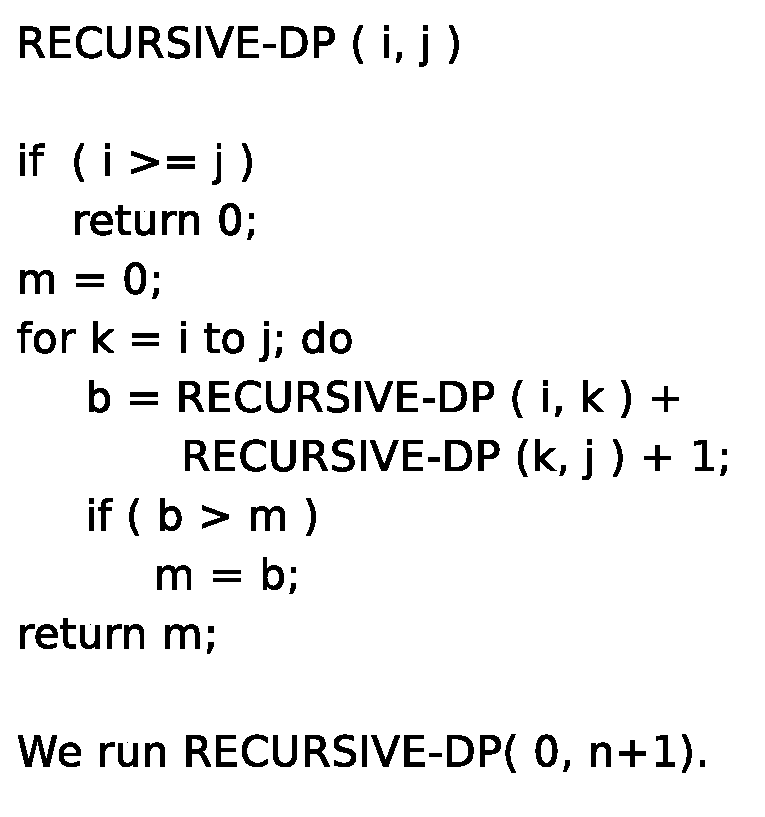
\includegraphics[width=1.0\textwidth]{L7-intervalschedulingdpalgo.eps}%
%      \end{minipage}%
%  \quad
%      \begin{minipage}{0.30\textwidth}
%       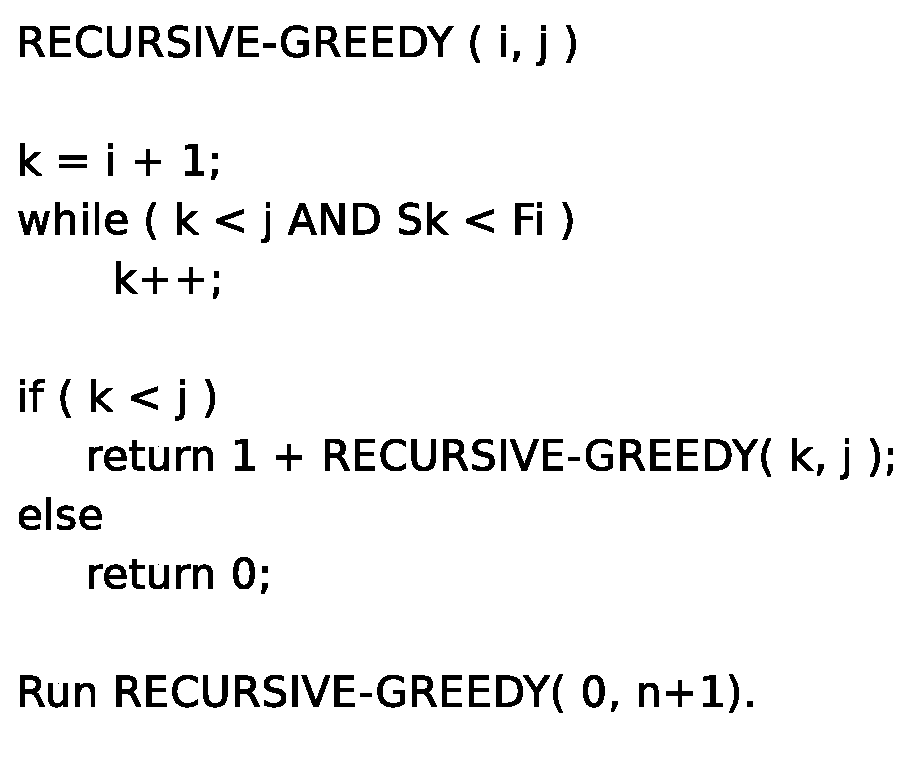
\includegraphics[width=1.0\textwidth]{L7-intervalschedulinggreedyalgo.eps}%
%      \end{minipage}%
%  \quad
%       \begin{minipage}{0.25\textwidth}
%       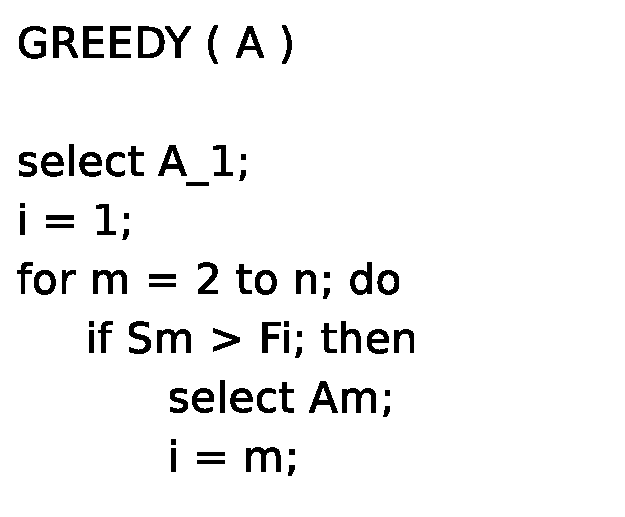
\includegraphics[width=1.0\textwidth]{L7-intervalschedulinggreedyalgo2.eps}%
%      \end{minipage}%
% 
%  \end{figure}

\title{CS711008Z  Algorithm Design and Analysis }
\subtitle{Lecture 10. Algorithm design technique: Network flow and its applications
%\footnote{The slides are made based on Chapter 7 of Introduction to algorithms, Combinatorial optimization algorithm and complexity by C. H. Papadimitriou and K. Steiglitz. Some slides are excerpted from the presentation by K. Wayne with permission.} 
}
\author{Dongbo Bu } 
\institute{{\small Institute of Computing Technology \\ 
Chinese Academy of Sciences, Beijing, China}}

\date{}

\begin{document}
%\begin{CJK}{UTF8}{cyberbit}



\frame{\titlepage}

\frame{
\frametitle{Outline}
\begin{itemize}
\item {\sc MaxFlow} problem: {\sc {\sc Ford-Fulkerson}} algorithm, {\sc {\sc MaxFlow-MinCut}} theorem; 
\item A duality explanation of {\sc {\sc Ford-Fulkerson}} algorithm and {\sc {\sc MaxFlow-MinCut}} theorem;
\item Efficient algorithms for {\sc MaxFlow} problem: scaling technique, {\sc {\sc Edmonds-Karp}} algorithm, {\sc Dinic's} algorithm (the original version and Even's version), {\sc Karzanov} algorithm and {\sc Push-Relabel} algorihtm;
%\item Solving the dual problem: Push-Relabel algorithm; 
%\item Connection with divide-and-conquer technique; 
\item Extensions of {\sc MaxFlow} problem: lower bound of capacity, multiple sources $\&$ multiple sinks, indirect graph. 
%\item Applications of network flow: {\sc BipartiteMatching}, {\sc ProteinDomainParsing}, {\sc BaseballElimination}, {\sc ImageSegmentation}, {\sc SurveyDesign}, {\sc FlightScheduling};
\end{itemize}

%Remarks: \\
%\begin{enumerate}
% \item The LP model of network flow problem can \textcolor{red}{automatically generate integral solution.}
% \item The powerful \textcolor{red}{scaling} technique can significantly reduce time-complexity from $O(mC)$ to $O(m^2 \log C)$. 
%%  \item 
%\end{enumerate}
}

\frame[allowframebreaks]{
\frametitle{A brief history of {\sc MinCut} problem }
\begin{figure}
 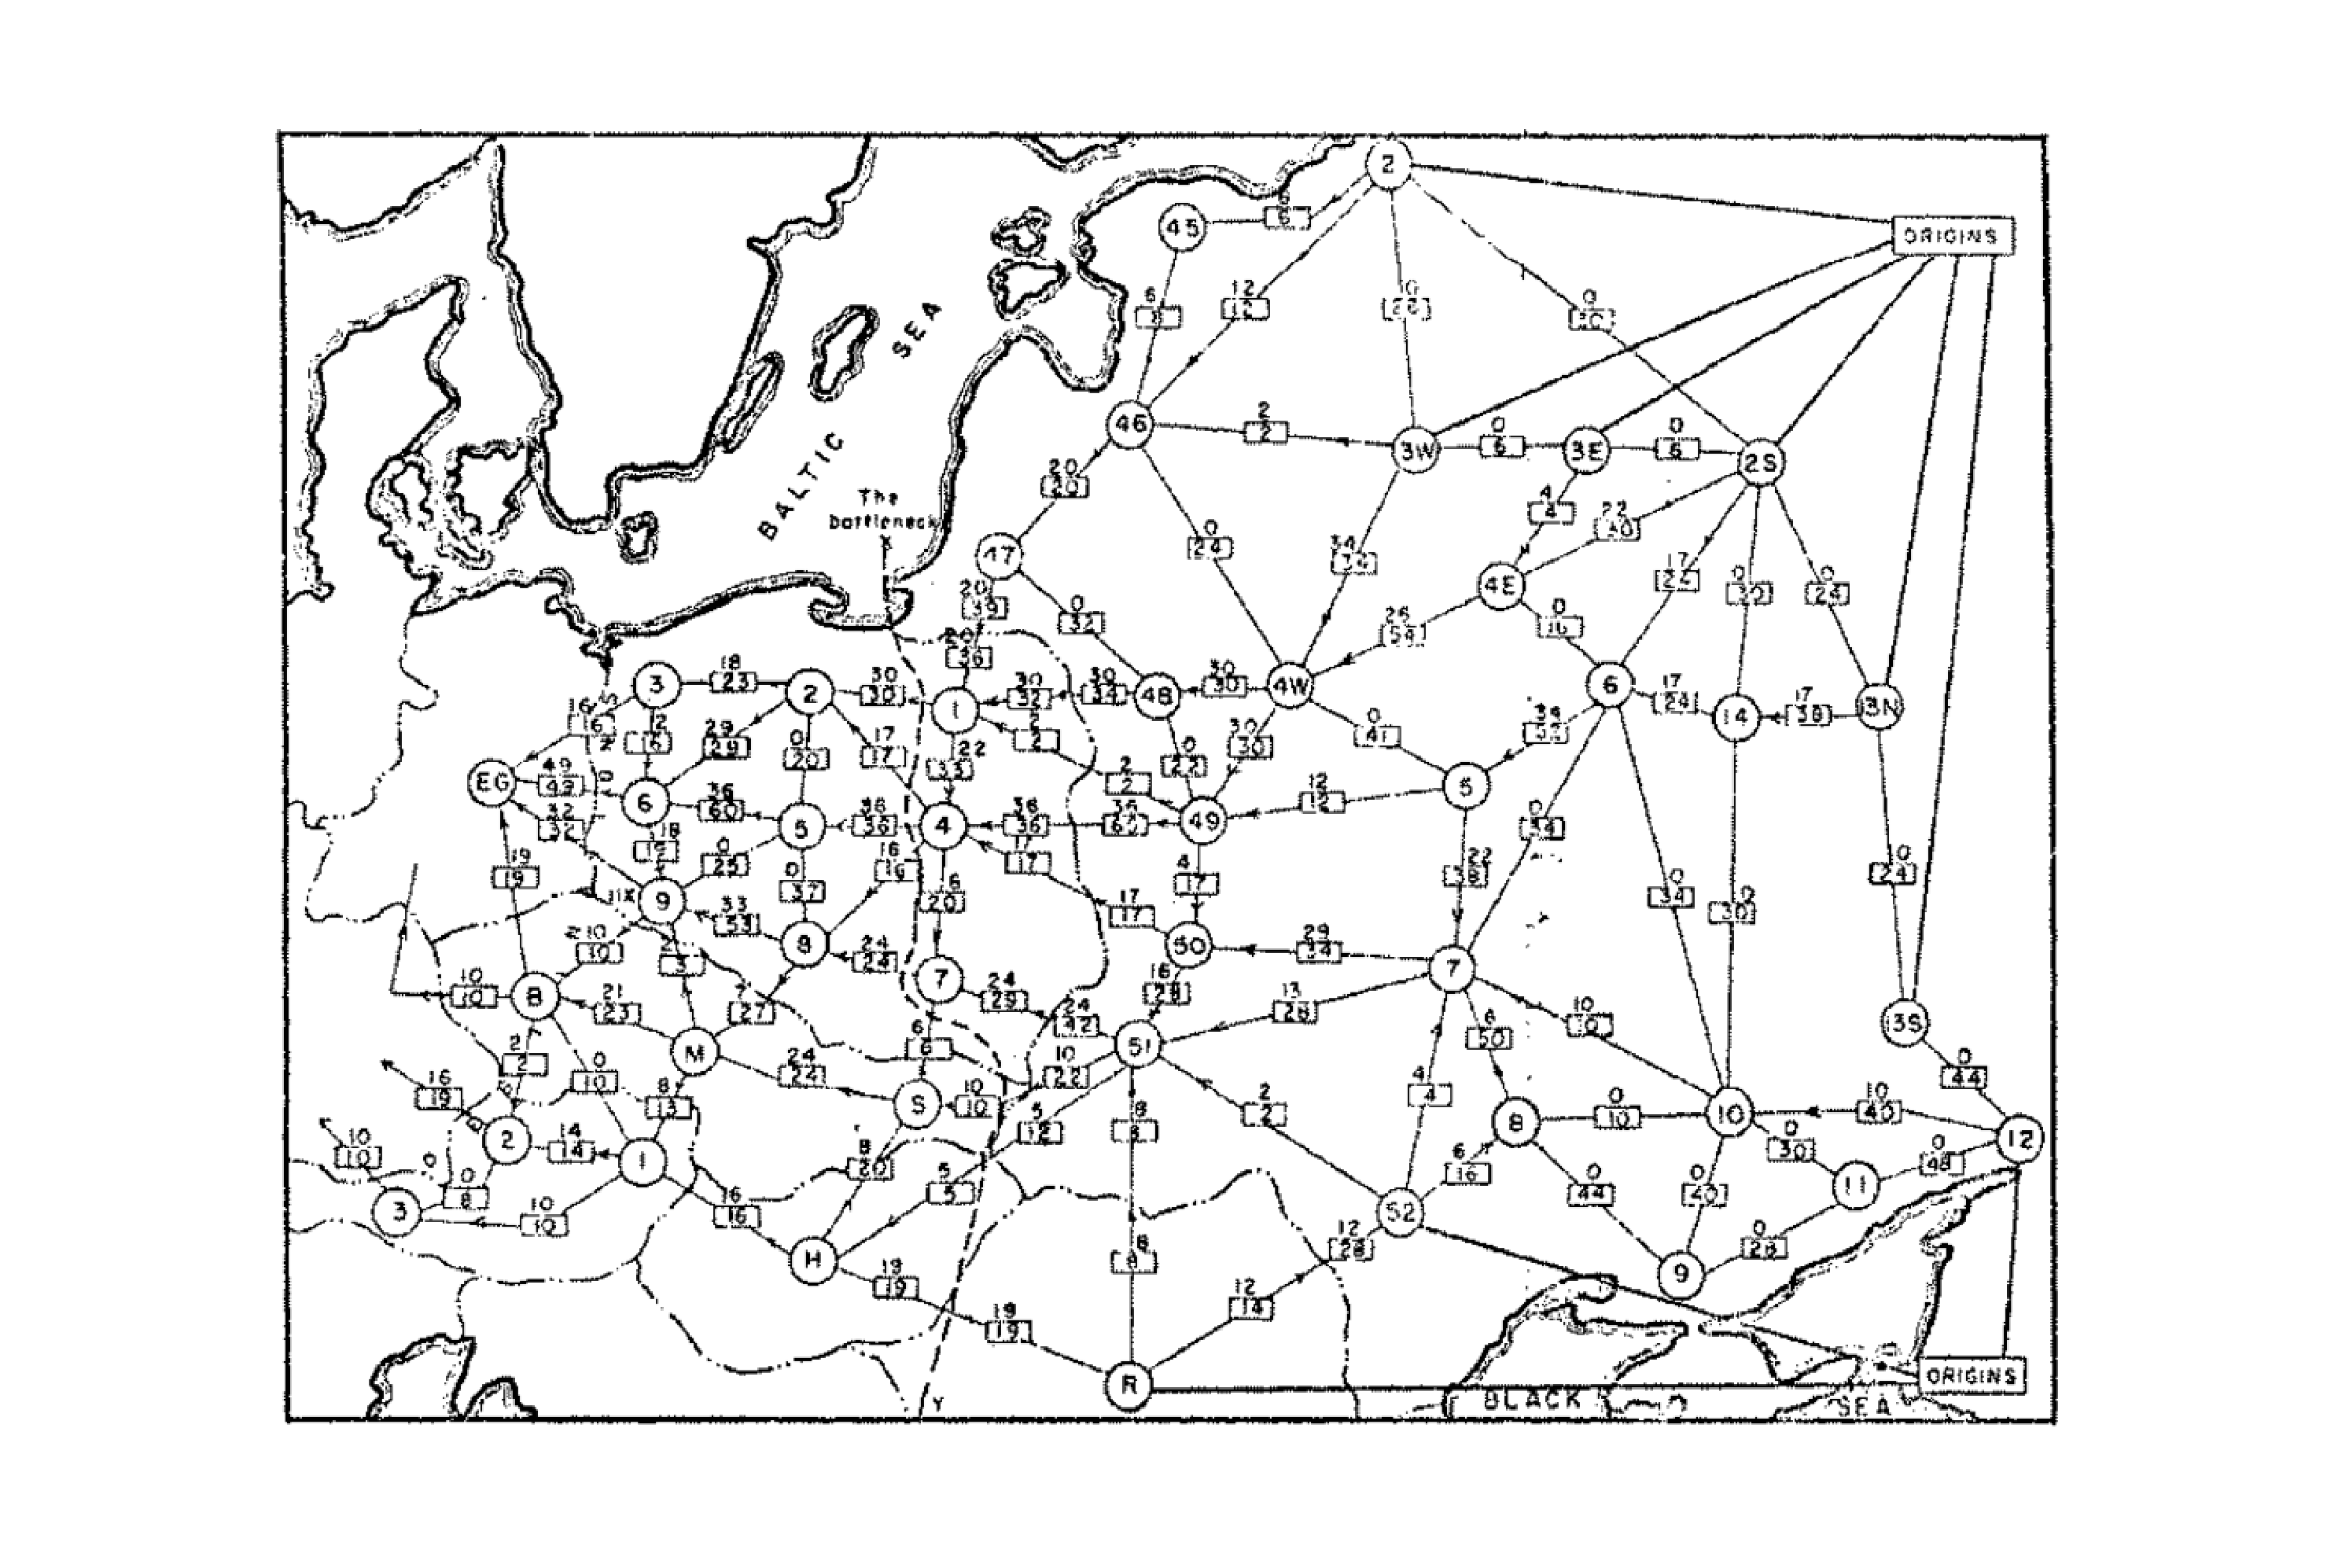
\includegraphics[width=3.5in] {L10-sovietunion.eps}
 \caption{Soviet Railway network, 1955}
\end{figure}

\begin{itemize}
 \item 
\textit{``From Harris and Ross [1955]: Schematic diagram of the railway network of the Western
Soviet Union and Eastern European countries, with a maximum flow of value 163,000 tons
from Russia to Eastern Europe, and a cut of capacity 163,000 tons indicated as `the
bottleneck' ...''}

\item
{A recently declassified U.S. Air Force report indicates that the original motivation of {\sc MinCut} problem and {\sc {\sc Ford-Fulkerson}} algorithm is \textcolor{red}{\it to disrupt rail transportation of the Soviet Union} [A. Shrijver, 2002]. }
\end{itemize}
}



\frame{
\begin{block}{}
 {\sc MaxFlow} problem and {\sc MinCut} problem 
\end{block}
}


\frame{
\frametitle{{\sc MaxFlow} problem }
\begin{block}{}
{\bf INPUT: }  \\
  A directed graph $G=<V, E>$. Each edge $e$ has a capacity $C_e$. Two special nodes: \textcolor{red}{\bf source} $s$ and \textcolor{red}{\bf sink} $t$;  \\
{\bf OUTPUT: } \\ 
 For each edge $e=(u, v)$, to assign a flow $f(u, v)$ such that $\sum_{u, (s,u)\in E} f{(s,u)}$ is maximized.
\end{block}

\begin{figure}
\begin{tikzpicture}[scale=1.3, auto,swap]
    % Draw a 7,11 network
    % First we draw the vertices
    \foreach \pos/\name in {{(0,0)/s}, {(2,1)/u}, {(2,-1)/v},
                            {(4,0)/t}}
        \node[middlevertex, draw,  fill=blue!20] (\name) at \pos {$\name$};
    % Connect vertices with edges and draw weights
    \foreach \source/ \dest /\weight in {s/u/{c_1=2}, u/t/{c_4=2},u/v/{c_3=3},s/v/{c_2=1},      v/t/{c_5=1} }
        \path[edge, sloped, midway, below, allow upside down] (\source) -- node[weight] {$\weight$} (\dest);
   \end{tikzpicture}
\end{figure}

Intuition: to push as many commodity as possible from \textcolor{red}{\bf source} $s$ to \textcolor{red}{\bf sink} $t$. 

} 

\frame{
\frametitle{$s-t$ flow}
\begin{figure}
\begin{tikzpicture}[scale=1.3, auto,swap]
    % Draw a 7,11 network
    % First we draw the vertices
    % Connect vertices with edges and draw weights
    \foreach \source/ \dest /\weight in {s/u/{1/2}, u/t/{0/2},u/v/{1/3},s/v/{0/1},      v/t/{1/1} }
        \path[edge, sloped, midway, below, allow upside down] (\source) -- node[weight] {$\weight$} (\dest);
    \path[draw, thick, ->, blue] (0, 0) -- (2,1);
         \path[draw, thick, ->, blue] (2,1) -- (2,-1);
             \path[draw, thick, ->, blue] (2, -1) -- (4, 0);
    \foreach \pos/\name in {{(0,0)/s}, {(2,1)/u}, {(2,-1)/v},
                            {(4,0)/t}}
        \node[middlevertex, draw,  fill=blue!20] (\name) at \pos {$\name$};

   \end{tikzpicture}
\end{figure}

\begin{definition}[$s-t$ flow]
$f: E\rightarrow R^+$ is a \textcolor{red}{\bf $s-t$ flow} if:
\begin{enumerate}
 \item (Capacity constraints): $0\leq f(e) \leq C_e$ for all edge $e$; \\
 \item (Conservation constraints): For any intermediate vertex $v \in V-\{s,t\}$, $f^{in}(v) = f^{out}(v)$, where $f^{in}(v) = \sum_{e \text{ into } v} f(e) $ and  $f^{out}(v) = \sum_{e \text{ out of } v} f(e)$. (Intuition: input = output for any intermediate vertex.)
\end{enumerate}
The \textcolor{red}{\bf value of flow $f$} is defined as $|f| = f^{out}(s)$. 
\end{definition}
}
%
%\frame{
%\frametitle{{\sc MaxFlow} problem: Example }
%
%\begin{figure}
%\begin{tikzpicture}[scale=1.3, auto,swap]
%    % Draw a 7,11 network
%    % First we draw the vertices
%    \foreach \pos/\name in {{(0,0)/s}, {(2,1)/u}, {(2,-1)/v},
%                            {(4,0)/t}}
%        \node[middlevertex, draw,  fill=blue!20] (\name) at \pos {$\name$};
%    % Connect vertices with edges and draw weights
%    \foreach \source/ \dest /\weight in {s/u/{c_1=2}, u/t/{c_4=2},u/v/{c_3=3},s/v/{c_2=1},      v/t/{c_5=1} }
%        \path[edge, sloped, midway, below, allow upside down] (\source) -- node[weight] {$\weight$} (\dest);
%   \end{tikzpicture}
%\end{figure}
%
%Notes: 
%\begin{enumerate}
%\item Dynamic programming doesn't seem to work.
% \item 
%We know that the {\sc MaxFlow} problem is in $\mathbf{P}$ since it can be  formulated as a linear program (See Lecture 8). 
%\item 
%However, the network structure has its own property to enable a  more efficient algorithm, informally called \textcolor{red}{\bf network simplex}, etc. 
%\end{enumerate}
%}

\frame{
\frametitle{{\sc MinCut} problem }
\begin{block}{}
{\bf INPUT: }  \\
  A directed graph $G=<V, E>$. Each edge $e$ has a capacity $C_e$. Two special nodes: \textcolor{red}{\bf source} $s$ and \textcolor{red}{\bf sink} $t$;  \\
{\bf OUTPUT: } \\ 
Find an $s-t$ cut with the minimum cut capacity. 
\end{block}

\begin{figure}
\begin{tikzpicture}[scale=1.3, auto,swap]
    % Draw a 7,11 network
    % First we draw the vertices

    % Connect vertices with edges and draw weights
    \foreach \source/ \dest /\weight in {s/u/{c_1=2}, u/t/{c_4=2},u/v/{c_3=3},s/v/{c_2=1},      v/t/{c_5=1} }
        \path[edge, sloped, midway, below, allow upside down] (\source) -- node[weight] {$\weight$} (\dest);
        
        \path[draw, thick, white, ->] (0,0)--(2,1);
        \path[draw, thick, white, ->] (2,-1)--(4,0);
        \path[draw, thick, green, ->] (0,0)--(2,1);
        \path[draw, thick, green, ->] (2,-1)--(4,0);
         \node[below, red] at (0, -0.5) {$\mathbf{S}$};
         \node[above, red] at (4, 0.5) {$\bar{\mathbf{S}}$};
         \path[draw, thick, dashed, red] (0.5,0.75)--(3.5,-0.75);
            \foreach \pos/\name in {{(0,0)/s}, {(2,1)/u}, {(2,-1)/v},{(4,0)/t}}
        \node[middlevertex, draw,  fill=blue!20] (\name) at \pos {$\name$};
        
   \end{tikzpicture}
\end{figure}
\begin{center}
$C(S, \bar{S}) = 3$
\end{center}


} 

\frame{
\frametitle{$s-t$ cut}

\begin{definition}[$s-t$ cut]
An \textcolor{red} {\bf $s-t$ cut} is a partition $(S, \bar{S})$ of $V$ such that $s\in S$ and $t \in \bar{S}$. The \textcolor{red}{\bf capacity of a cut $(S, \bar{S})$} is defined as $C(S, \bar{S}) = \sum_{e \text{ from }S\text{ to }\bar{S}} C(e)$. 
\end{definition} 

\begin{figure}
\begin{tikzpicture}[scale=1.3, auto,swap]
    % Draw a 7,11 network
    % First we draw the vertices

    % Connect vertices with edges and draw weights
    \foreach \source/ \dest /\weight in {s/u/{c_1=2}, u/t/{c_4=2},u/v/{c_3=3},s/v/{c_2=1},      v/t/{c_5=1} }
        \path[edge, sloped, midway, below, allow upside down] (\source) -- node[weight] {$\weight$} (\dest);
        
        \path[draw, thick, white, ->] (0,0)--(2,1);
        \path[draw, thick, white, ->] (2,-1)--(4,0);
        \path[draw, thick, green, ->] (0,0)--(2,1);
        \path[draw, thick, green, ->] (2,-1)--(4,0);
         \node[below, red] at (0, -0.5) {$\mathbf{S}$};
         \node[above, red] at (4, 0.5) {$\bar{\mathbf{S}}$};
         \path[draw, thick, dashed, red] (0.5,0.75)--(3.5,-0.75);
            \foreach \pos/\name in {{(0,0)/s}, {(2,1)/u}, {(2,-1)/v},{(4,0)/t}}
        \node[middlevertex, draw,  fill=blue!20] (\name) at \pos {$\name$};
        
   \end{tikzpicture}
\end{figure}
\begin{center}
$C(S, \bar{S}) = 3$
\end{center}
}


%\frame{
%\frametitle{Intuition} 
%Hint: Consider the three cases of edge $e=(u,v)$: \\
%\begin{enumerate}
% \item $A\rightarrow A$ ( $u, v \in A$):   $f(e)$ appears in both $f^{out}(v)$ and $-f^{in}(v)$ and thus was cancelled out.
% \item $A\rightarrow B$ ($u \in A, v\notin A$): $f(e)$ appears in $f^{out}(v)$ only. 
% \item $\bar{S}\rightarrow S$ ($u \notin A, v \in A$): $f(e)$ appears in $-f^{in}(v)$ only.
%\end{enumerate}
%
%\begin{figure}
% 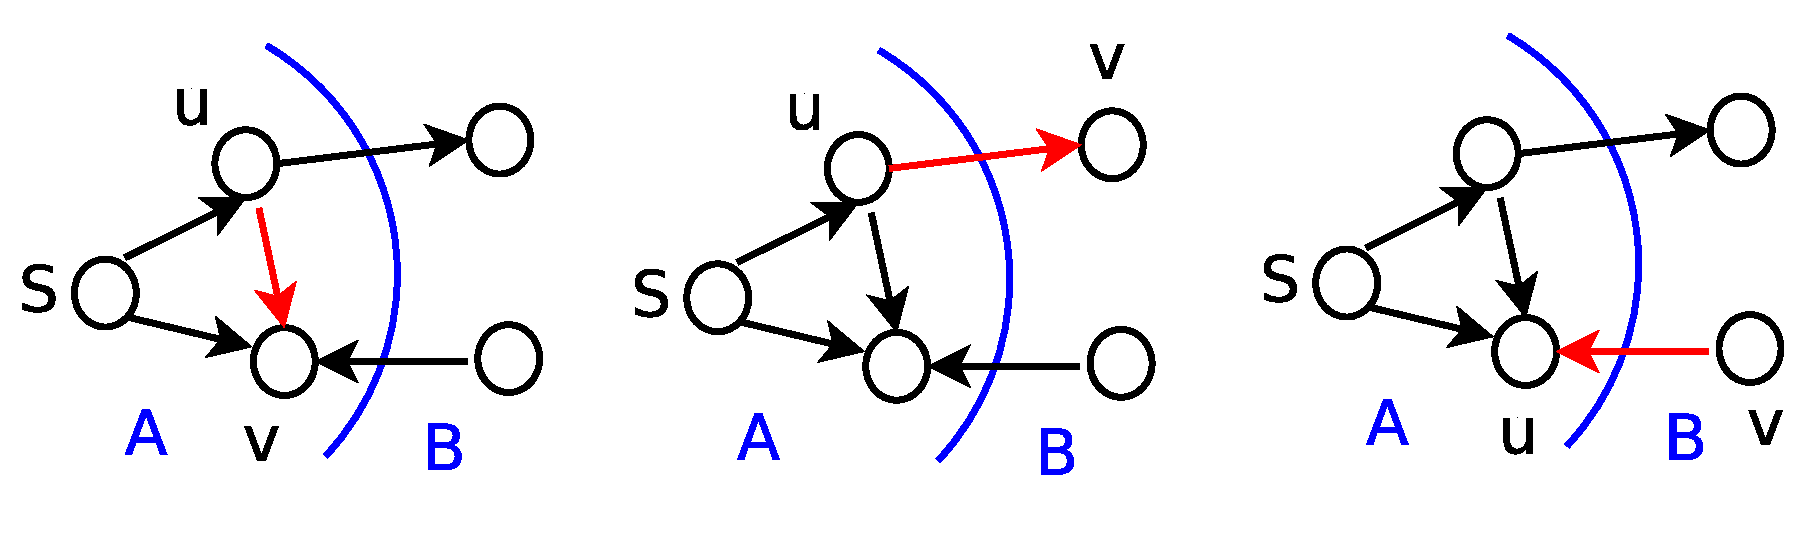
\includegraphics[width=3.5in] {L10-flowvaluelemma.eps}
%\end{figure}
%}

\frame{
\frametitle{A brief history of algorithms to {\sc MinCut} problem }

 \begin{table}
   {\begin{tabular}{lcc}\hline
%        & \multicolumn{3}{c}{Actual number of DCJ operations}\\
        Year  & Developers &  Time-complexity  \\
\hline
1956 & L. R. Ford and D. R. Fulkerson & $O(m C)$  \\ 
%and $O(m^2\log C)$ \\
1970 & Y. Dinitz & $O( m n^2)$ \\
1972 & J. Edmonds and R. Karp & $O(m^2 n)$ \\
1974 & A. Karzanov & $O(n^3)$ \\
%1986 & Sleator and Tarjan & $O(nm \log n)$ \\
1986 & A. Goldberg and R. Tarjan & $O(mn^2)$, $O(n^3)$, $O(m n \log(\frac{n^{2}}{m}))$ \\ 
2013  & J. Orlin	& $O(mn)$ \\ \hline
 
     \end{tabular}} {}%
 \end{table}
} 

\frame{
\begin{block}{}
 {\sc {\sc Ford-Fulkerson}} algorithm  [1956]
\end{block}
}

\frame{
\frametitle{Lester Randolph Ford Jr. and Delbert Ray Fulkerson }

 \begin{figure}%
   \begin{center}%
     \begin{minipage}{0.40\textwidth}%
      
\includegraphics[width=1.0\textwidth]{FordJr.png}%
     \end{minipage}%
     \qquad
     \begin{minipage}{0.40\textwidth}
      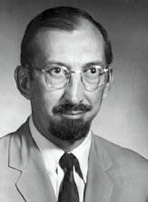
\includegraphics[width=1.0\textwidth]{Fulkerson.png}%
     \end{minipage}%
   \end{center}
   \caption{Lester Randolph Ford Jr. and Delbert Ray Fulkerson} 
 \end{figure} 
}


\frame{
\frametitle{Trial 1: Dynamic programming technique}


\begin{itemize}
\item 
Dynamic programming doesn't seem to work as it is not easy to define appropriate sub-problems.  
In fact, there is no efficient algorithm known for {\sc Maximum Flow} problem that can really be viewed as belonging to the dynamic programming paradigm. 
 \item 
We know that the {\sc MaxFlow} problem is in $\mathbf{P}$ since it can be  formulated as a linear program (See Lecture 8).  
However, the network structure has its own property to enable a  more efficient algorithm, informally called \textcolor{red}{\bf network simplex}.  In addition, special-purpose algorithms are more efficient. 
\end{itemize}

} 


\frame{
\frametitle{Trial 2: {\sc Improvement} strategy }

\begin{itemize}

\item Let's return to  the general {\sc Improvement} strategy: 



{\sc Improvement}$(f)$
\begin{algorithmic}[1]
\STATE ${x=x_0}$; //starting from an initial solution;
\WHILE{\texttt{TRUE} }
\STATE ${x}=${\sc Improve}$({x})$; //move one step towards optimum;
\IF{{\sc Stopping}$({x}, f)$ }
\STATE break;
\ENDIF
\ENDWHILE
\RETURN ${x}$;
\end{algorithmic}

\end{itemize}
}

\frame{
\frametitle{Three key questions of {\sc Improvement} strategy} 
\begin{itemize}
\item 
Three key questions: 
\begin{enumerate} 
\item How to construct an initial solution?  
	\begin{itemize}
	\item For {\sc MaxFlow} problem,  an initial solution can be easily obtained by setting $f(e)=0$ for any $e$ (called $0-$flow). It is easy to verify that both {\sc conservation} and {\sc capacity} constraints hold for the 0-flow. 
	\end{itemize}
\item How to improve a solution? 
\item When shall we stop? 
\end{enumerate} 
\end{itemize}

} 


\frame{
\frametitle{A failure start: augmenting flow along a path in the original graph }

 \begin{itemize}
 \item 
Let $p$ be a simple ${s-t}$ path in the network $G$. 

  \begin{algorithmic}[1]
    \STATE Initialize $f(e)=0$ for all $e$.
    \WHILE{there is an  $s-t$ path  in graph $G$}
    \STATE  \textcolor{red}{\bf Arbitrarily} choose an $s-t$ path $p$ in graph $G$;  
    \STATE $f = ${\sc augment}$(p, f)$;
    \ENDWHILE
    \RETURN{$f$};
  \end{algorithmic}
\end{itemize} 

} 

\frame{
\frametitle{Augmenting flow along a path  }

 \begin{itemize}
 \item 
We define $bottleneck(p, f)$ as the minimum residual capacity of edges in path $p$. 

{\sc augment}$(p, f)$\\
  \begin{algorithmic}[1]
  \STATE Let $b=bottleneck(p, f);$
    \FOR{each edge $e=(u,v)$ $\in p$}
%    \IF{$(u,v)$ is a forward edge}
    \STATE Increase $f(u,v)$ by $b;$
%    \ELSE
%    \STATE decrease $f(u,v)$ by $b;$
%    \ENDIF
    \ENDFOR
  \end{algorithmic}
\end{itemize}
} 

\frame{
\frametitle{Why we failed? }

\begin{itemize}
 \item 
Consider the following example. We start from 0-flow and find a $s-t$ path in $G$, say $p = s\rightarrow u  \rightarrow v  \rightarrow t$, to transmit one more unit of commodity to increase the value of $f$.  
\item 
However we cannot find a $s-t$ path in $G$ again to increase $f$ further (left panel) although  the maximum flow value is $2$ (right panel). 

\end{itemize}


\begin{figure}
\begin{tikzpicture}[scale=1, auto,swap]

    \def\dx{0};
    \def\dy{0};	

     \foreach \x/\y/\name in {0/0/s, 2/1/u, 2/-1/v, 4/0/t}
        \node[middlevertex, draw,  fill=blue!20] (\name) at (\x+\dx, \y+\dy) {$\name$};
        
        
    \foreach \source/ \dest /\weight in {s/u/{1/1}}
        \path[edge, sloped, midway, above, allow upside down, blue] (\source) -- node[weight] {\small $\weight$} (\dest);
        
    \foreach \source/ \dest /\weight in {u/t/{0/1}}
        \path[edge, sloped, midway, above, allow upside down] (\source) -- node[weight] {\small $\weight$} (\dest);        
        
    \foreach \source/ \dest /\weight in {u/v/{1/1}}
        \path[edge, sloped, midway, above, allow upside down, blue] (\source) -- node[weight] {\small $\weight$} (\dest);
        
    \foreach \source/ \dest /\weight in {v/t/{1/1}}
        \path[edge, sloped, midway, below, allow upside down, blue] (\source) -- node[weight] {\small $\weight$} (\dest);

    \foreach \source/ \dest /\weight in {s/v/{0/1}}
        \path[edge, sloped, midway, below, allow upside down] (\source) -- node[weight] {\small $\weight$} (\dest);
       \node[ultra thick, red, below] at (v.south) {$|f|=1$};          
        
        
    \def\dx{5};
    \def\dy{0};	

     \foreach \x/\y/\name in {0/0/s, 2/1/u, 2/-1/v, 4/0/t}
        \node[middlevertex, draw,  fill=blue!20] (\name) at (\x+\dx, \y+\dy) {$\name$};
        
        
    \foreach \source/ \dest /\weight in {s/u/{1/1}}
        \path[edge, sloped, midway, above, allow upside down, blue] (\source) -- node[weight] {\small $\weight$} (\dest);
        
    \foreach \source/ \dest /\weight in {u/t/{1/1}}
        \path[edge, sloped, midway, above, allow upside down, blue] (\source) -- node[weight] {\small $\weight$} (\dest);        
        
    \foreach \source/ \dest /\weight in {u/v/{0/1}}
        \path[edge, sloped, midway, above, allow upside down ] (\source) -- node[weight] {\small $\weight$} (\dest);
        
    \foreach \source/ \dest /\weight in {v/t/{1/1}}
        \path[edge, sloped, midway, below, allow upside down, blue] (\source) -- node[weight] {\small $\weight$} (\dest);

    \foreach \source/ \dest /\weight in {s/v/{1/1}}
        \path[edge, sloped, midway, below, allow upside down, blue] (\source) -- node[weight] {\small $\weight$} (\dest);
       
    \node[ultra thick, red, below] at (v.south) {$|f|=2$};     
        
   \end{tikzpicture}
\end{figure}

%\begin{figure}
% \includegraphics[width=4.5in] {L10-networkflowexample-graph.eps}
%\end{figure}
}

\frame{
\frametitle{{\sc Ford-Fulkerson} algorithm: \textcolor{red}{\bf ``undo''} functionality } 
 \begin{itemize}
 \item 
Key observation:
\begin{itemize}
 \item  
 When constructing a flow $f$, one  might commit errors on some edges, i.e. the edges should not  be used to transmit commodity. For example, the edge $u\rightarrow v$ should  not be used. 



\begin{figure}
\begin{tikzpicture}[scale=1, auto,swap]

    \def\dx{0};
    \def\dy{0};	

     \foreach \x/\y/\name in {0/0/s, 2/1/u, 2/-1/v, 4/0/t}
        \node[middlevertex, draw,  fill=blue!20] (\name) at (\x+\dx, \y+\dy) {$\name$};
        
        
    \foreach \source/ \dest /\weight in {s/u/{1/1}}
        \path[edge, sloped, midway, above, allow upside down, blue] (\source) -- node[weight] {\small $\weight$} (\dest);
        
    \foreach \source/ \dest /\weight in {u/t/{0/1}}
        \path[edge, sloped, midway, above, allow upside down] (\source) -- node[weight] {\small $\weight$} (\dest);        
        
    \foreach \source/ \dest /\weight in {u/v/{1/1}}
        \path[edge, sloped, midway, above, allow upside down, red] (\source) -- node[weight] {\small $\weight$} (\dest);
        
    \foreach \source/ \dest /\weight in {v/t/{1/1}}
        \path[edge, sloped, midway, below, allow upside down, blue] (\source) -- node[weight] {\small $\weight$} (\dest);

    \foreach \source/ \dest /\weight in {s/v/{0/1}}
        \path[edge, sloped, midway, below, allow upside down] (\source) -- node[weight] {\small $\weight$} (\dest);
       \node[ultra thick, red, below] at (v.south) {$|f|=1$};          
        
        
%    \def\dx{5};
%    \def\dy{0};	
%
%     \foreach \x/\y/\name in {0/0/s, 2/1/u, 2/-1/v, 4/0/t}
%        \node[middlevertex, draw,  fill=blue!20] (\name) at (\x+\dx, \y+\dy) {$\name$};
%        
%        
%    \foreach \source/ \dest /\weight in {s/u/{1/1}}
%        \path[edge, sloped, midway, above, allow upside down, blue] (\source) -- node[weight] {\small $\weight$} (\dest);
%        
%    \foreach \source/ \dest /\weight in {u/t/{1/1}}
%        \path[edge, sloped, midway, above, allow upside down, blue] (\source) -- node[weight] {\small $\weight$} (\dest);        
%        
%    \foreach \source/ \dest /\weight in {u/v/{0/1}}
%        \path[edge, sloped, midway, above, allow upside down ] (\source) -- node[weight] {\small $\weight$} (\dest);
%        
%    \foreach \source/ \dest /\weight in {v/t/{1/1}}
%        \path[edge, sloped, midway, below, allow upside down, blue] (\source) -- node[weight] {\small $\weight$} (\dest);
%
%    \foreach \source/ \dest /\weight in {s/v/{1/1}}
%        \path[edge, sloped, midway, below, allow upside down, blue] (\source) -- node[weight] {\small $\weight$} (\dest);
%       
%    \node[ultra thick, red, below] at (v.south) {$|f|=2$};     
        
   \end{tikzpicture}
\end{figure}

 \item 
  To improve the current flow $f$, we should work out ways to \textcolor{red}{\bf correct these errors}, i.e. ``undo'' the transmission assigned on the edges. 
\end{itemize}
\end{itemize}

} 

\frame{
\frametitle{Implementing the  \textcolor{red}{``undo''} functionality } 

\begin{itemize}
 \item  But how to implement the \textcolor{red}{``undo''}  functionality? 
 \item   \textcolor{red}{\bf Adding backward  edges! } 
 \item Suppose we add a \textcolor{red}{\bf backward} edge $v\rightarrow u$ into the original graph. Then we can correct the transmission via pushing back commodity from $v$ to $u$. 
 \end{itemize}
 
 \begin{figure}
\begin{tikzpicture}[scale=1, auto,swap]

    \def\dx{0};
    \def\dy{0};	

     \foreach \x/\y/\name in {0/0/s, 2/1/u, 2/-1/v, 4/0/t}
        \node[middlevertex, draw,  fill=blue!20] (\name) at (\x+\dx, \y+\dy) {$\name$};
        
        
    \foreach \source/ \dest /\weight in {s/u/{1/1}}
        \path[edge, sloped, midway, above, allow upside down, blue] (\source) -- node[weight] {\small $\weight$} (\dest);
        
    \foreach \source/ \dest /\weight in {u/t/{0/1}}
        \path[edge, sloped, midway, above, allow upside down] (\source) -- node[weight] {\small $\weight$} (\dest);        
        
    \foreach \source/ \dest /\weight in {u/v/{1/1}}
        \path[edge, sloped, midway, above, allow upside down, blue] (\source) -- node[weight] {\small $\weight$} (\dest);
        
    \foreach \source/ \dest /\weight in {v/t/{1/1}}
        \path[edge, sloped, midway, below, allow upside down, blue] (\source) -- node[weight] {\small $\weight$} (\dest);

    \foreach \source/ \dest /\weight in {s/v/{0/1}}
        \path[edge, sloped, midway, below, allow upside down] (\source) -- node[weight] {\small $\weight$} (\dest);
       \node[ultra thick, blue, below] at (v.south) {Flow $f$};          
        
        
    \def\dx{5};
    \def\dy{0};	

     \foreach \x/\y/\name in {0/0/s, 2/1/u, 2/-1/v, 4/0/t}
        \node[middlevertex, draw,  fill=blue!20] (\name) at (\x+\dx, \y+\dy) {$\name$};
        
        \draw[->, thick] (s.15) -- node[below, sloped, midway] {\small $0$} (u.225);
        \draw[->, thick, red] (u.195) -- node[above, sloped, midway] {\small $1$} (s.45);

        \draw[->, thick] (u.285) -- node[above, sloped, midway] {\small $0$} (v.75);
        \draw[->, thick, red] (v.105) -- node[above, sloped, midway] {\small $1$} (u.255);

        \draw[->, thick] (v.15) -- node[below, sloped, midway] {\small $0$} (t.225);
        \draw[->, thick, red] (t.195) -- node[above, sloped, midway] {\small $1$} (v.45);

        
%    \foreach \source/ \dest /\weight in {s/u/{1/1}}
%        \path[edge, sloped, midway, above, allow upside down, blue] (\source) -- node[weight] {\small $\weight$} (\dest);
        
    \foreach \source/ \dest /\weight in {u/t/{1}}
        \path[edge, sloped, midway, above, allow upside down, black] (\source) -- node[weight] {\small $\weight$} (\dest);        
        
%    \foreach \source/ \dest /\weight in {u/v/{0/1}}
%        \path[edge, sloped, midway, above, allow upside down ] (\source) -- node[weight] {\small $\weight$} (\dest);
        
%    \foreach \source/ \dest /\weight in {v/t/{1/1}}
%        \path[edge, sloped, midway, below, allow upside down, blue] (\source) -- node[weight] {\small $\weight$} (\dest);

    \foreach \source/ \dest /\weight in {s/v/{1}}
        \path[edge, sloped, midway, below, allow upside down, black] (\source) -- node[weight] {\small $\weight$} (\dest);
       
   \node[ultra thick, red, below] at (v.south) {Backward edges};     
         
   \end{tikzpicture}
\end{figure}

% \begin{figure}
% 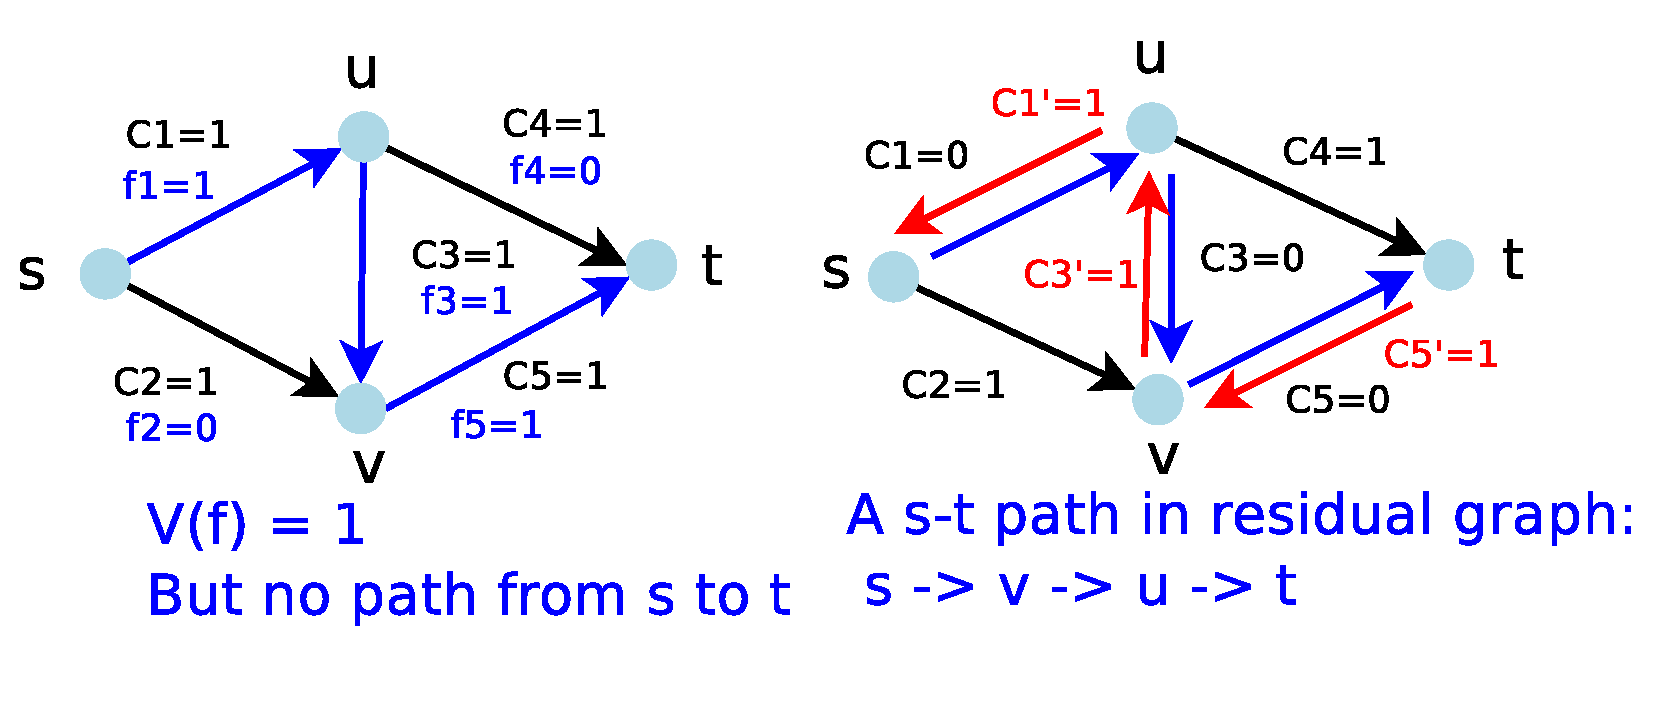
\includegraphics[width=3.5in] {L10-networkflowexampleresidualgraph.eps}
%\end{figure}
}


\frame{
\frametitle{Residual graph with \textcolor{red}{\bf ``backward"} edges to correct errors } 
% \begin{figure}
% 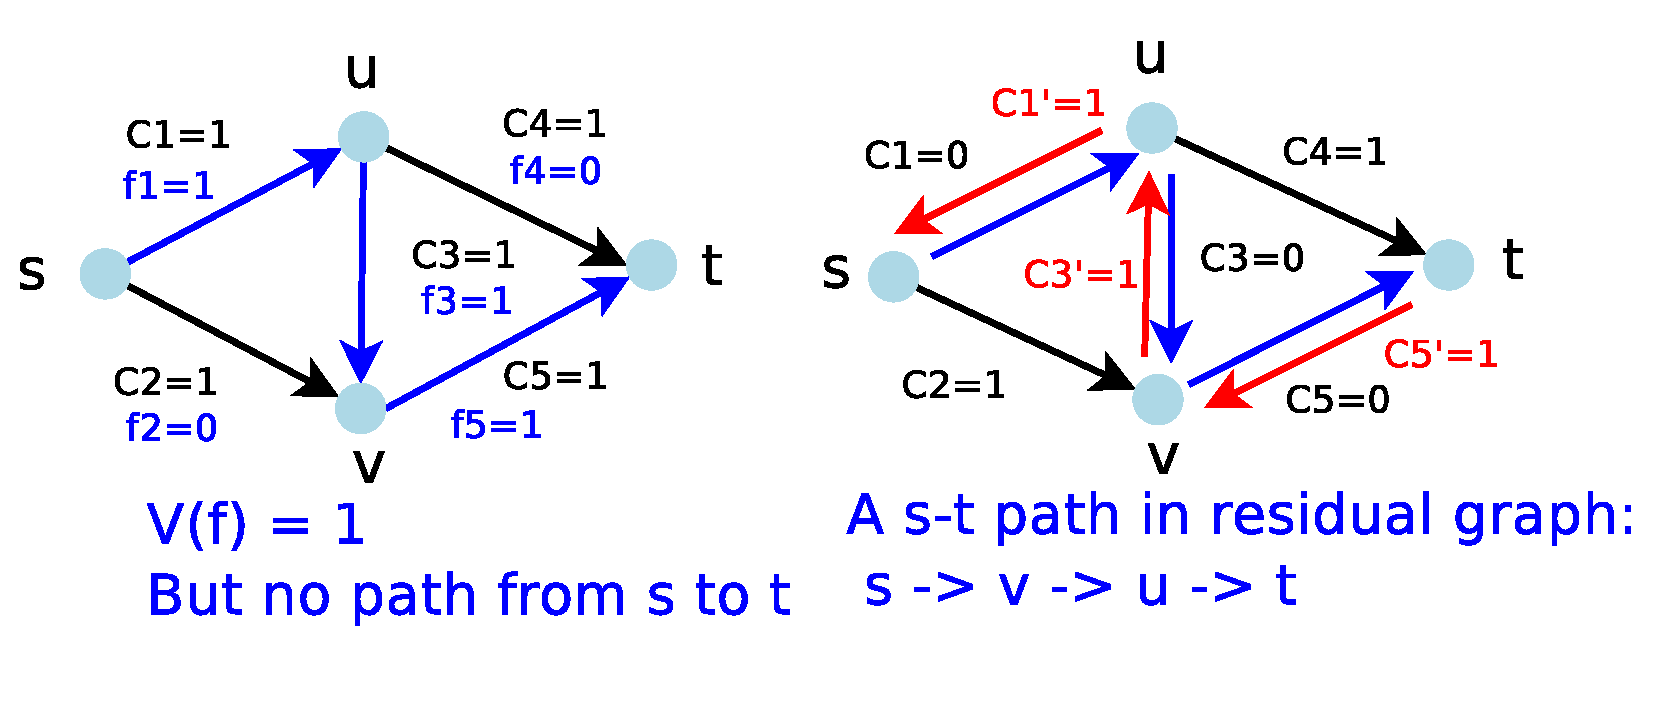
\includegraphics[width=4.4in] {L10-networkflowexampleresidualgraph.eps}
%\end{figure}
\begin{definition}[Residual Graph]
   Given a directed graph $G=<V,E>$ with a flow $f$, we define \textcolor{red}{\bf residual graph} $G_f=<V, E'>$. For any edge $e = (u,v) \in E$, two edges are added into $E'$ as follows: 
\begin{enumerate}
\begin{small}
 \item \textcolor{red}{\bf Forward edge} $(u, v)$ with residual capacity: \\
If $f(e) < C(e)$,  edge $e=(u,v)$ will be added to $G'$ with capacity $C(e)=C(e) - f(e)$. 
 \item \textcolor{red}{\bf Backward edge}  $(v, u)$ with undo capacity: \\
If $f(e) > 0$,  edge $e'=(v,u)$ will be added to $G'$ with capacity $C(e') = f(e)$. 
\end{small}
\end{enumerate}
\end{definition}
}

%\frame{
%\frametitle {An example: $f$ and $G_f$ } 
%\begin{figure}
% \includegraphics[width=2in] {L10-networkflowunderstandingresidualgraph1.eps}
%\end{figure}
%} 

\frame{
\frametitle {Finding an $s-t$ path in $G_f$ rather than $G$ } 

 \begin{figure}
\begin{tikzpicture}[scale=1, auto,swap]

    \def\dx{0};
    \def\dy{0};	

     \foreach \x/\y/\name in {0/0/s, 2/1/u, 2/-1/v, 4/0/t}
        \node[middlevertex, draw,  fill=blue!20] (\name) at (\x+\dx, \y+\dy) {$\name$};
        
        
    \foreach \source/ \dest /\weight in {s/u/{1/1}}
        \path[edge, sloped, midway, above, allow upside down, blue] (\source) -- node[weight] {\small $\weight$} (\dest);
        
    \foreach \source/ \dest /\weight in {u/t/{0/1}}
        \path[edge, sloped, midway, above, allow upside down] (\source) -- node[weight] {\small $\weight$} (\dest);        
        
    \foreach \source/ \dest /\weight in {u/v/{1/1}}
        \path[edge, sloped, midway, above, allow upside down, blue] (\source) -- node[weight] {\small $\weight$} (\dest);
        
    \foreach \source/ \dest /\weight in {v/t/{1/1}}
        \path[edge, sloped, midway, below, allow upside down, blue] (\source) -- node[weight] {\small $\weight$} (\dest);

    \foreach \source/ \dest /\weight in {s/v/{0/1}}
        \path[edge, sloped, midway, below, allow upside down] (\source) -- node[weight] {\small $\weight$} (\dest);
       \node[ultra thick, blue, below] at (v.south) {Flow $f$};          
        
        
    \def\dx{5};
    \def\dy{0};	

     \foreach \x/\y/\name in {0/0/s, 2/1/u, 2/-1/v, 4/0/t}
        \node[middlevertex, draw,  fill=blue!20] (\name) at (\x+\dx, \y+\dy) {$\name$};
        
        \draw[->, thick] (s.15) -- node[below, sloped, midway] {\small $0$} (u.225);
        \draw[->, thick] (u.195) -- node[above, sloped, midway] {\small $1$} (s.45);

        \draw[->, thick] (u.285) -- node[above, sloped, midway] {\small $0$} (v.75);
        \draw[->, thick, green] (v.105) -- node[above, sloped, midway, green] {\small $1$} (u.255);

        \draw[->, thick] (v.15) -- node[below, sloped, midway] {\small $0$} (t.225);
        \draw[->, thick] (t.195) -- node[above, sloped, midway] {\small $1$} (v.45);

        
%    \foreach \source/ \dest /\weight in {s/u/{1/1}}
%        \path[edge, sloped, midway, above, allow upside down, blue] (\source) -- node[weight] {\small $\weight$} (\dest);
        
    \foreach \source/ \dest /\weight in {u/t/{1}}
        \path[edge, sloped, midway, above, allow upside down, green] (\source) -- node[weight] {\small $\weight$} (\dest);        
        
%    \foreach \source/ \dest /\weight in {u/v/{0/1}}
%        \path[edge, sloped, midway, above, allow upside down ] (\source) -- node[weight] {\small $\weight$} (\dest);
        
%    \foreach \source/ \dest /\weight in {v/t/{1/1}}
%        \path[edge, sloped, midway, below, allow upside down, blue] (\source) -- node[weight] {\small $\weight$} (\dest);

    \foreach \source/ \dest /\weight in {s/v/{1}}
        \path[edge, sloped, midway, below, allow upside down, green] (\source) -- node[weight] {\small $\weight$} (\dest);
       
   \node[ultra thick, red, below] at (v.south) {Residual graph $G_f$};     
        
   \end{tikzpicture}
\end{figure}



%
%\begin{figure}
% \includegraphics[width=1.95in] {L10-networkflowunderstandingresidualgraph2.eps}
%\end{figure}
\begin{itemize}
\item 
Note that we cannot find an $s-t$ path in $G$; however, we can find an $s-t$ path \textcolor{green}{$s\rightarrow v \rightarrow u \rightarrow t$} in $G_{f}$, which contains a backward edge $(v,u)$.  
\end{itemize}

}

\frame{
\frametitle {Augmenting the flow  $f$ along an $s-t$ path in $G_{f}$ } 



 \begin{figure}
\begin{tikzpicture}[scale=0.8, auto,swap]

    \def\dx{0};
    \def\dy{0};	

     \foreach \x/\y/\name in {0/0/s, 2/1/u, 2/-1/v, 4/0/t}
        \node[middlevertex, draw,  fill=blue!20] (\name) at (\x+\dx, \y+\dy) {$\name$};
        
        
    \foreach \source/ \dest /\weight in {s/u/{1/1}}
        \path[edge, sloped, midway, above, allow upside down, blue] (\source) -- node[weight] {\small $\weight$} (\dest);
        
    \foreach \source/ \dest /\weight in {u/t/{0/1}}
        \path[edge, sloped, midway, above, allow upside down] (\source) -- node[weight] {\small $\weight$} (\dest);        
        
    \foreach \source/ \dest /\weight in {u/v/{1/1}}
        \path[edge, sloped, midway, above, allow upside down, blue] (\source) -- node[weight] {\small $\weight$} (\dest);
        
    \foreach \source/ \dest /\weight in {v/t/{1/1}}
        \path[edge, sloped, midway, below, allow upside down, blue] (\source) -- node[weight] {\small $\weight$} (\dest);

    \foreach \source/ \dest /\weight in {s/v/{0/1}}
        \path[edge, sloped, midway, below, allow upside down] (\source) -- node[weight] {\small $\weight$} (\dest);
       \node[ultra thick, blue, below] at (v.south) {Flow $f$};          
        
       \node[ultra thick, blue] at (4, -1.7 ) {\large +}; 
       
    \def\dx{5};
    \def\dy{0};	

     \foreach \x/\y/\name in {0/0/s, 2/1/u, 2/-1/v, 4/0/t}
        \node[middlevertex, draw,  fill=blue!20] (\name) at (\x+\dx, \y+\dy) {$\name$};
        
        \draw[->, thick] (s.15) -- node[below, sloped, midway] {\small $0$} (u.225);
        \draw[->, thick] (u.195) -- node[above, sloped, midway] {\small $1$} (s.45);

        \draw[->, thick] (u.285) -- node[above, sloped, midway] {\small $0$} (v.75);
        \draw[->, thick, green] (v.105) -- node[above, sloped, midway, green] {\small $1$} (u.255);

        \draw[->, thick] (v.15) -- node[below, sloped, midway] {\small $0$} (t.225);
        \draw[->, thick] (t.195) -- node[above, sloped, midway] {\small $1$} (v.45);

        
%    \foreach \source/ \dest /\weight in {s/u/{1/1}}
%        \path[edge, sloped, midway, above, allow upside down, blue] (\source) -- node[weight] {\small $\weight$} (\dest);
        
    \foreach \source/ \dest /\weight in {u/t/{1}}
        \path[edge, sloped, midway, above, allow upside down, green] (\source) -- node[weight] {\small $\weight$} (\dest);        
        
%    \foreach \source/ \dest /\weight in {u/v/{0/1}}
%        \path[edge, sloped, midway, above, allow upside down ] (\source) -- node[weight] {\small $\weight$} (\dest);
        
%    \foreach \source/ \dest /\weight in {v/t/{1/1}}
%        \path[edge, sloped, midway, below, allow upside down, blue] (\source) -- node[weight] {\small $\weight$} (\dest);

    \foreach \source/ \dest /\weight in {s/v/{1}}
        \path[edge, sloped, midway, below, allow upside down, green] (\source) -- node[weight] {\small $\weight$} (\dest);
       
   \node[ultra thick, green, below] at (v.south) {An $s-t$ path in $G_f$};     


      \node[ultra thick, blue] at (10, -1.75) {\large =}; 

       
    \def\dx{10};
    \def\dy{0};	

     \foreach \x/\y/\name in {0/0/s, 2/1/u, 2/-1/v, 4/0/t}
        \node[middlevertex, draw,  fill=blue!20] (\name) at (\x+\dx, \y+\dy) {$\name$};
        
%        \draw[->, thick] (s.15) -- node[below, sloped, midway] {\small $0$} (u.225);
%        \draw[->, thick] (u.195) -- node[above, sloped, midway] {\small $1$} (s.45);
%
%        \draw[->, thick] (u.285) -- node[above, sloped, midway] {\small $0$} (v.75);
%        \draw[->, thick, green] (v.105) -- node[above, sloped, midway, green] {\small $1$} (u.255);
%
%        \draw[->, thick] (v.15) -- node[below, sloped, midway] {\small $0$} (t.225);
%        \draw[->, thick] (t.195) -- node[above, sloped, midway] {\small $1$} (v.45);

        
    \foreach \source/ \dest /\weight in {s/u/{1/1}}
        \path[edge, sloped, midway, above, allow upside down, blue] (\source) -- node[weight] {\small $\weight$} (\dest);
        
    \foreach \source/ \dest /\weight in {u/t/{1/1}}
        \path[edge, sloped, midway, above, allow upside down, green] (\source) -- node[weight] {\small $\weight$} (\dest);        
        
    \foreach \source/ \dest /\weight in {u/v/{0/1}}
        \path[edge, sloped, midway, above, allow upside down ] (\source) -- node[weight] {\small $\weight$} (\dest);
        
    \foreach \source/ \dest /\weight in {v/t/{1/1}}
        \path[edge, sloped, midway, below, allow upside down, blue] (\source) -- node[weight] {\small $\weight$} (\dest);

    \foreach \source/ \dest /\weight in {s/v/{1/1}}
        \path[edge, sloped, midway, below, allow upside down, green] (\source) -- node[weight] {\small $\weight$} (\dest);
       
   \node[ultra thick, red, below] at (v.south) {New flow $f'$};     


        
   \end{tikzpicture}
\end{figure}




%\begin{figure}
% \includegraphics[width=4.5in] {L10-networkflowunderstandingresidualgraph3.eps}
%\end{figure}


\begin{itemize}
\item 
By using the backward edge $v\rightarrow u$, the initial transmission from $u$ to $v$ is pushed back.  
\item More specifically, 
 the first commodity transferred through flow $f$ changes its path (from $s\rightarrow u\rightarrow v\rightarrow t$ to $s\rightarrow u\rightarrow t$), while the second one uses the path $s\rightarrow v\rightarrow t$. 
 \end{itemize}
}


\frame{
\frametitle{{\sc {\sc Ford-Fulkerson}} algorithm  }

 \begin{itemize}
 \item 
Let $p$ be a simple ${s-t}$ path in residual graph $G_f$, called \textcolor{red}{\bf augmentation path}. We define $bottleneck(p, f)$ as the minimum  capacity of edges in path $p$. 

\ \\
{\sc {\sc Ford-Fulkerson}} algorithm:\\
  \begin{algorithmic}[1]
    \STATE Initialize $f(e)=0$ for all $e$.
    \WHILE{there is an  $s-t$ path  in residual graph $G_f$}
    \STATE  \textcolor{red}{\bf Arbitrarily} choose an $s-t$ path $p$ in $G_f$;  
    \STATE $f = ${\sc augment}$(p, f)$;
    \ENDWHILE
    \RETURN{$f$};
  \end{algorithmic}
\end{itemize} 

} 



\frame{
\begin{block}{}
Correctness and time-complexity analysis
\end{block}

}

\frame{
\frametitle{Property 1: augmentation generates a new flow}



\begin{lemma}
 The operation $f'=${\sc augment}$(p, f)$ generates a new flow $f'$ in $G$. 
\end{lemma}
%\begin{figure}
% \includegraphics[width=4in] {L10-networkflowunderstandingresidualgraph3.eps}
%\end{figure}


 \begin{figure}
\begin{tikzpicture}[scale=0.8, auto,swap]

    \def\dx{0};
    \def\dy{0};	

     \foreach \x/\y/\name in {0/0/s, 2/1/u, 2/-1/v, 4/0/t}
        \node[middlevertex, draw,  fill=blue!20] (\name) at (\x+\dx, \y+\dy) {$\name$};
        
        
    \foreach \source/ \dest /\weight in {s/u/{1/1}}
        \path[edge, sloped, midway, above, allow upside down, blue] (\source) -- node[weight] {\small $\weight$} (\dest);
        
    \foreach \source/ \dest /\weight in {u/t/{0/1}}
        \path[edge, sloped, midway, above, allow upside down] (\source) -- node[weight] {\small $\weight$} (\dest);        
        
    \foreach \source/ \dest /\weight in {u/v/{1/1}}
        \path[edge, sloped, midway, above, allow upside down, blue] (\source) -- node[weight] {\small $\weight$} (\dest);
        
    \foreach \source/ \dest /\weight in {v/t/{1/1}}
        \path[edge, sloped, midway, below, allow upside down, blue] (\source) -- node[weight] {\small $\weight$} (\dest);

    \foreach \source/ \dest /\weight in {s/v/{0/1}}
        \path[edge, sloped, midway, below, allow upside down] (\source) -- node[weight] {\small $\weight$} (\dest);
       \node[ultra thick, blue, below] at (v.south) {Flow $f$};          
        
       \node[ultra thick, blue] at (4, -1.7 ) {\large +}; 
       
    \def\dx{5};
    \def\dy{0};	

     \foreach \x/\y/\name in {0/0/s, 2/1/u, 2/-1/v, 4/0/t}
        \node[middlevertex, draw,  fill=blue!20] (\name) at (\x+\dx, \y+\dy) {$\name$};
        
        \draw[->, thick] (s.15) -- node[below, sloped, midway] {\small $0$} (u.225);
        \draw[->, thick] (u.195) -- node[above, sloped, midway] {\small $1$} (s.45);

        \draw[->, thick] (u.285) -- node[above, sloped, midway] {\small $0$} (v.75);
        \draw[->, thick, green] (v.105) -- node[above, sloped, midway, green] {\small $1$} (u.255);

        \draw[->, thick] (v.15) -- node[below, sloped, midway] {\small $0$} (t.225);
        \draw[->, thick] (t.195) -- node[above, sloped, midway] {\small $1$} (v.45);

        
%    \foreach \source/ \dest /\weight in {s/u/{1/1}}
%        \path[edge, sloped, midway, above, allow upside down, blue] (\source) -- node[weight] {\small $\weight$} (\dest);
        
    \foreach \source/ \dest /\weight in {u/t/{1}}
        \path[edge, sloped, midway, above, allow upside down, green] (\source) -- node[weight] {\small $\weight$} (\dest);        
        
%    \foreach \source/ \dest /\weight in {u/v/{0/1}}
%        \path[edge, sloped, midway, above, allow upside down ] (\source) -- node[weight] {\small $\weight$} (\dest);
        
%    \foreach \source/ \dest /\weight in {v/t/{1/1}}
%        \path[edge, sloped, midway, below, allow upside down, blue] (\source) -- node[weight] {\small $\weight$} (\dest);

    \foreach \source/ \dest /\weight in {s/v/{1}}
        \path[edge, sloped, midway, below, allow upside down, green] (\source) -- node[weight] {\small $\weight$} (\dest);
       
   \node[ultra thick, green, below] at (v.south) {An $s-t$ path in $G_f$};     


      \node[ultra thick, blue] at (10, -1.75) {\large =}; 

       
    \def\dx{10};
    \def\dy{0};	

     \foreach \x/\y/\name in {0/0/s, 2/1/u, 2/-1/v, 4/0/t}
        \node[middlevertex, draw,  fill=blue!20] (\name) at (\x+\dx, \y+\dy) {$\name$};
        
%        \draw[->, thick] (s.15) -- node[below, sloped, midway] {\small $0$} (u.225);
%        \draw[->, thick] (u.195) -- node[above, sloped, midway] {\small $1$} (s.45);
%
%        \draw[->, thick] (u.285) -- node[above, sloped, midway] {\small $0$} (v.75);
%        \draw[->, thick, green] (v.105) -- node[above, sloped, midway, green] {\small $1$} (u.255);
%
%        \draw[->, thick] (v.15) -- node[below, sloped, midway] {\small $0$} (t.225);
%        \draw[->, thick] (t.195) -- node[above, sloped, midway] {\small $1$} (v.45);

        
    \foreach \source/ \dest /\weight in {s/u/{1/1}}
        \path[edge, sloped, midway, above, allow upside down, blue] (\source) -- node[weight] {\small $\weight$} (\dest);
        
    \foreach \source/ \dest /\weight in {u/t/{1/1}}
        \path[edge, sloped, midway, above, allow upside down, green] (\source) -- node[weight] {\small $\weight$} (\dest);        
        
    \foreach \source/ \dest /\weight in {u/v/{0/1}}
        \path[edge, sloped, midway, above, allow upside down ] (\source) -- node[weight] {\small $\weight$} (\dest);
        
    \foreach \source/ \dest /\weight in {v/t/{1/1}}
        \path[edge, sloped, midway, below, allow upside down, blue] (\source) -- node[weight] {\small $\weight$} (\dest);

    \foreach \source/ \dest /\weight in {s/v/{1/1}}
        \path[edge, sloped, midway, below, allow upside down, green] (\source) -- node[weight] {\small $\weight$} (\dest);
       
   \node[ultra thick, red, below] at (v.south) {New flow $f'$};     


        
   \end{tikzpicture}
\end{figure}


} 

\frame{
\frametitle{}
%\begin{figure}
% \includegraphics[width=4in] {L10-networkflowunderstandingresidualgraph3.eps}
%\end{figure}


\begin{Proof}
 \begin{itemize}
  \item Checking \textcolor{red}{\bf capacity constraints}:  Let's examine the following two cases of edge $e=(u,v)$ in path $p$. 
\begin{enumerate}
\item $(u,v)$ is a forward edge arising from $(u,v)\in E$: \\
$0\leq f(e) \leq f'(e) = f(e) + bottleneck(p, f) \leq f(e) + (C(e) - f(e)) \leq C(e)$.
\item $(u,v) $ is a backward edge arising from $(v,u) \in E $: \\
$C(e) \geq f(e) \geq f'(e) = f(e) - bottleneck(p, f) \geq f(e) - f(e) = 0$.
\end{enumerate}
  
  \item Checking \textcolor{red}{\bf conservation constraints}: 
For each node $v$, the change of the amount of flow entering $v$ is the same as the change in the amount of flow exiting $v$.
\end{itemize} 
\end{Proof}

}

\frame{
\frametitle{Property 2: Monotonically increasing }
\begin{lemma}  
$|f'|> |f|$. 
\end{lemma}

 \begin{figure}
\begin{tikzpicture}[scale=0.8, auto,swap]

    \def\dx{0};
    \def\dy{0};	

     \foreach \x/\y/\name in {0/0/s, 2/1/u, 2/-1/v, 4/0/t}
        \node[middlevertex, draw,  fill=blue!20] (\name) at (\x+\dx, \y+\dy) {$\name$};
        
        
    \foreach \source/ \dest /\weight in {s/u/{1/1}}
        \path[edge, sloped, midway, above, allow upside down, blue] (\source) -- node[weight] {\small $\weight$} (\dest);
        
    \foreach \source/ \dest /\weight in {u/t/{0/1}}
        \path[edge, sloped, midway, above, allow upside down] (\source) -- node[weight] {\small $\weight$} (\dest);        
        
    \foreach \source/ \dest /\weight in {u/v/{1/1}}
        \path[edge, sloped, midway, above, allow upside down, blue] (\source) -- node[weight] {\small $\weight$} (\dest);
        
    \foreach \source/ \dest /\weight in {v/t/{1/1}}
        \path[edge, sloped, midway, below, allow upside down, blue] (\source) -- node[weight] {\small $\weight$} (\dest);

    \foreach \source/ \dest /\weight in {s/v/{0/1}}
        \path[edge, sloped, midway, below, allow upside down] (\source) -- node[weight] {\small $\weight$} (\dest);
       \node[ultra thick, blue, below] at (v.south) {Flow $f$};          
        
       \node[ultra thick, blue] at (4, -1.7 ) {\large +}; 
       
    \def\dx{5};
    \def\dy{0};	

     \foreach \x/\y/\name in {0/0/s, 2/1/u, 2/-1/v, 4/0/t}
        \node[middlevertex, draw,  fill=blue!20] (\name) at (\x+\dx, \y+\dy) {$\name$};
        
        \draw[->, thick] (s.15) -- node[below, sloped, midway] {\small $0$} (u.225);
        \draw[->, thick] (u.195) -- node[above, sloped, midway] {\small $1$} (s.45);

        \draw[->, thick] (u.285) -- node[above, sloped, midway] {\small $0$} (v.75);
        \draw[->, thick, green] (v.105) -- node[above, sloped, midway, green] {\small $1$} (u.255);

        \draw[->, thick] (v.15) -- node[below, sloped, midway] {\small $0$} (t.225);
        \draw[->, thick] (t.195) -- node[above, sloped, midway] {\small $1$} (v.45);

        
%    \foreach \source/ \dest /\weight in {s/u/{1/1}}
%        \path[edge, sloped, midway, above, allow upside down, blue] (\source) -- node[weight] {\small $\weight$} (\dest);
        
    \foreach \source/ \dest /\weight in {u/t/{1}}
        \path[edge, sloped, midway, above, allow upside down, green] (\source) -- node[weight] {\small $\weight$} (\dest);        
        
%    \foreach \source/ \dest /\weight in {u/v/{0/1}}
%        \path[edge, sloped, midway, above, allow upside down ] (\source) -- node[weight] {\small $\weight$} (\dest);
        
%    \foreach \source/ \dest /\weight in {v/t/{1/1}}
%        \path[edge, sloped, midway, below, allow upside down, blue] (\source) -- node[weight] {\small $\weight$} (\dest);

    \foreach \source/ \dest /\weight in {s/v/{1}}
        \path[edge, sloped, midway, below, allow upside down, green] (\source) -- node[weight] {\small $\weight$} (\dest);
       
   \node[ultra thick, green, below] at (v.south) {An $s-t$ path in $G_f$};     


      \node[ultra thick, blue] at (10, -1.75) {\large =}; 

       
    \def\dx{10};
    \def\dy{0};	

     \foreach \x/\y/\name in {0/0/s, 2/1/u, 2/-1/v, 4/0/t}
        \node[middlevertex, draw,  fill=blue!20] (\name) at (\x+\dx, \y+\dy) {$\name$};
        
%        \draw[->, thick] (s.15) -- node[below, sloped, midway] {\small $0$} (u.225);
%        \draw[->, thick] (u.195) -- node[above, sloped, midway] {\small $1$} (s.45);
%
%        \draw[->, thick] (u.285) -- node[above, sloped, midway] {\small $0$} (v.75);
%        \draw[->, thick, green] (v.105) -- node[above, sloped, midway, green] {\small $1$} (u.255);
%
%        \draw[->, thick] (v.15) -- node[below, sloped, midway] {\small $0$} (t.225);
%        \draw[->, thick] (t.195) -- node[above, sloped, midway] {\small $1$} (v.45);

        
    \foreach \source/ \dest /\weight in {s/u/{1/1}}
        \path[edge, sloped, midway, above, allow upside down, blue] (\source) -- node[weight] {\small $\weight$} (\dest);
        
    \foreach \source/ \dest /\weight in {u/t/{1/1}}
        \path[edge, sloped, midway, above, allow upside down, green] (\source) -- node[weight] {\small $\weight$} (\dest);        
        
    \foreach \source/ \dest /\weight in {u/v/{0/1}}
        \path[edge, sloped, midway, above, allow upside down ] (\source) -- node[weight] {\small $\weight$} (\dest);
        
    \foreach \source/ \dest /\weight in {v/t/{1/1}}
        \path[edge, sloped, midway, below, allow upside down, blue] (\source) -- node[weight] {\small $\weight$} (\dest);

    \foreach \source/ \dest /\weight in {s/v/{1/1}}
        \path[edge, sloped, midway, below, allow upside down, green] (\source) -- node[weight] {\small $\weight$} (\dest);
       
   \node[ultra thick, red, below] at (v.south) {New flow $f'$};     


        
   \end{tikzpicture}
\end{figure}

\begin{itemize}
 \item 
Hint: $|f'|=|f| + bottleneck(p,f) > |f|$ since  $bottleneck(p,f) > 0$. 
\end{itemize}
} 

\frame{
\frametitle{Property 3: a trivial upper bound of flow  }

\begin{lemma} 
$|f|$ has an upper bound $C=\sum_{e\text{ out of }s} C(e)$. 
\end{lemma}
(Intuition: the edges out of $s$ are completely saturated by  flow $f$.)

\begin{figure}
\begin{tikzpicture}[scale=1.3, auto,swap]
    % Draw a 7,11 network
    % First we draw the vertices
    \foreach \pos/\name in {{(0,0)/s}, {(2,1)/u}, {(2,-1)/v},
                            {(4,0)/t}}
        \node[middlevertex, draw,  fill=blue!20] (\name) at \pos {$\name$};
    % Connect vertices with edges and draw weights
    \foreach \source/ \dest /\weight in {s/u/{c_1=2}, u/t/{c_4=2},u/v/{c_3=3},s/v/{c_2=1},      v/t/{c_5=1} }
        \path[edge, sloped, midway, below, allow upside down] (\source) -- node[weight] {$\weight$} (\dest);
   \end{tikzpicture}
\end{figure}

} 

\frame{
\frametitle{Property 4: Augmentation  step  }

\begin{Theorem} 
Assume all edges have integer capacities, thus at every intermediate stage of the execution of  {\sc {\sc Ford-Fulkerson}} algorithm, both flow value $|f|$ and residual capacities are integers, and  $bottleneck(p, f) \geq 1$. There will be at most $C$ iterations of the {\tt while}  loop. 
\end{Theorem}

\begin{itemize}
\item 
Time complexity: $O(mC)$. 
	 \begin{itemize}
 		\item $O(C)$ iterations: Under a reasonable assumption that all capacities are integers, $bottleneck(p, f) \geq 1 $ at each iteration and thus $|f'| \geq |f| + 1$.
		\item At each iteration, it takes $O(m+n)$ time to find an $s-t$ path in $G_f$  using DFS or BFS technique.
	\end{itemize}
\item Note that the bound is not polynomial as $C$ is exponential in the size of problem input.  A polynomial  algorithm is one with a worst-case time bound polynomial in $n$, $m$, and $\log C$ (the number of bits to represent $C$). We assume that elementary arithmetic operations take unit time and algorithms manipulate numbers that fit in a machine word.	
\end{itemize}
}

\frame{
\frametitle{Property 5: A tighter upper bound  }
%Recall  \textit{Flow value lemma}: Let $f$ be any flow, and $(S, \bar{S})$ be any cut. Then the flow across the cut is equal to $|f|$, i.e., $|f| = f^{out}(S) - f^{in} (S)$. 


\begin{theorem}  
Consider a flow $f$ and an $s-t$ cut $(S, \bar{S})$.  We have $|f| \leq C(S, \bar{S})$. 
\end{theorem}

\begin{figure}
\begin{tikzpicture}[scale=1.3, auto,swap]
    % Draw a 7,11 network
    % First we draw the vertices

    % Connect vertices with edges and draw weights
    \foreach \source/ \dest /\weight in {s/u/{2/2}, u/t/{1/2},u/v/{1/3},s/v/{0/1},      v/t/{1/1} }
        \path[edge, sloped, midway, below, allow upside down] (\source) -- node[weight] {$\weight$} (\dest);
        
        \path[draw, thick, green, ->] (0,0)--(2,1);
        \path[draw, thick, green, ->] (2,-1)--(4,0);
        \path[draw, thick, blue, ->] (2,1)--(2,-1);  
    %    \path[draw, thick, dashed, red] (0.5, 0.5)--(0.5, -0.6);      
         \node[below, red] at (0, -0.5) {$\mathbf{S}$};
         \node[above, red] at (4, 0.5) {$\bar{\mathbf{S}}$};
         \path[draw, thick, dashed, red] (0.5,0.75)--(3.5,-0.75);
            \foreach \pos/\name in {{(0,0)/s}, {(2,1)/u}, {(2,-1)/v},{(4,0)/t}}
        \node[middlevertex, draw,  fill=blue!20] (\name) at \pos {$\name$};
        
   \end{tikzpicture}
\end{figure}
\begin{centering}
\qquad \qquad \qquad \qquad \qquad $|f|=2$ $\leq$   $C(S, \bar{S}) = 3$
\end{centering}

} 

\frame{
\begin{figure}
\begin{tikzpicture}[scale=1.3, auto,swap]
    % Draw a 7,11 network
    % First we draw the vertices

    % Connect vertices with edges and draw weights
    \foreach \source/ \dest /\weight in {s/u/{2/2}, u/t/{1/2},u/v/{1/3},s/v/{0/1},      v/t/{1/1} }
        \path[edge, sloped, midway, below, allow upside down] (\source) -- node[weight] {$\weight$} (\dest);
        
        \path[draw, thick, green, ->] (0,0)--(2,1);
        \path[draw, thick, green, ->] (2,-1)--(4,0);
        \path[draw, thick, blue, ->] (2,1)--(2,-1);  
       % \path[draw, thick, dashed, red] (0.5, 0.5)--(0.5, -0.6);      
         \node[below, red] at (0, -0.5) {$\mathbf{S}$};
         \node[above, red] at (4, 0.5) {$\bar{\mathbf{S}}$};
         \path[draw, thick, dashed, red] (0.5,0.75)--(3.5,-0.75);
            \foreach \pos/\name in {{(0,0)/s}, {(2,1)/u}, {(2,-1)/v},{(4,0)/t}}
        \node[middlevertex, draw,  fill=blue!20] (\name) at \pos {$\name$};
        
   \end{tikzpicture}
\end{figure}

\begin{Proof}
\begin{footnotesize}
\begin{eqnarray}
|f| &=& f^{out}(S) - f^{in}(S)   \qquad \text{(by flow value lemma)}	 \nonumber \\
     &\textcolor{red}{\leq}& f^{out}(S)   \text{\qquad\qquad\qquad  (by } f^{in}(S)\geq 0 )\nonumber \\
     &=& \sum\nolimits_{\text{e $\in S\rightarrow \bar{S}$}} f(e)  \nonumber \\
     &\textcolor{red}{\leq}&  \sum\nolimits_{\text{e $\in S\rightarrow \bar{S}$}} C(e)  \text{\qquad (by } f(e) \leq C(e) )  \nonumber  \\
     &=& C(S, \bar{S})  \nonumber 
\end{eqnarray} 
\end{footnotesize}
\end{Proof}
}

\frame{
\frametitle{Flow value lemma}


\begin{lemma}{}  
Consider an $s-t$ flow  $f$ and any $s-t$ cut $(S, \bar{S})$. The flow  across the cut is a constant $|f|$. Formally,  $|f| = f^{out}(S) - f^{in} (S)$. 
\end{lemma}

\begin{figure}
\begin{tikzpicture}[scale=1.3, auto,swap]
    % Draw a 7,11 network
    % First we draw the vertices

    % Connect vertices with edges and draw weights
    \foreach \source/ \dest /\weight in {s/u/{2/2}, u/t/{1/2},u/v/{1/3},s/v/{0/1},      v/t/{1/1} }
        \path[edge, sloped, midway, below, allow upside down] (\source) -- node[weight] {$\weight$} (\dest);
        
        \path[draw, thick, green, ->] (0,0)--(2,1);
        \path[draw, thick, green, ->] (2,-1)--(4,0);
        \path[draw, thick, blue, ->] (2,1)--(2,-1);  
        \path[draw, thick, dashed, red] (0.5, 0.5)--(0.5, -0.6);      
         \node[below, red] at (0, -0.5) {$\mathbf{S}$};
         \node[above, red] at (4, 0.5) {$\bar{\mathbf{S}}$};
         \path[draw, thick, dashed, red] (0.5,0.75)--(3.5,-0.75);
            \foreach \pos/\name in {{(0,0)/s}, {(2,1)/u}, {(2,-1)/v},{(4,0)/t}}
        \node[middlevertex, draw,  fill=blue!20] (\name) at \pos {$\name$};
        
   \end{tikzpicture}
\end{figure}
\begin{center}
$|f| = 2 + 0 = 2$\\
$f^{out}(S) - f^{in}(S) = 2 + 1 - 1 = |f|$
\end{center}


} 

\frame{
\frametitle{}
\begin{figure}
\begin{tikzpicture}[scale=1.3]
    % Draw a 7,11 network
    % First we draw the vertices

    % Connect vertices with edges and draw weights
    \foreach \source/ \dest /\weight in {s/u/{2/2}, u/t/{1/2},u/v/{1/3},s/v/{0/1},      v/t/{1/1} }
        \path[edge, sloped, midway, below, allow upside down] (\source) -- node[weight] {$\weight$} (\dest);     
        \path[draw, thick, green, ->] (0,0)--(2,1);
        \path[draw, thick, green, ->] (2,-1)--(4,0);
        \path[draw, thick, blue, ->] (2,1)--(2,-1);        
         \node[below, red] at (0, -0.5) {$\mathbf{S}$};
         \node[above, red] at (4, 0.5) {$\bar{\mathbf{S}}$};
         \path[draw, thick, dashed, red] (0.5,0.75)--(3.5,-0.75);
                 \path[draw, thick, dashed, red] (0.5, 0.5)--(0.5, -0.6);     
            \foreach \pos/\name in {{(0,0)/s}, {(2,1)/u}, {(2,-1)/v},{(4,0)/t}}
        \node[middlevertex, draw,  fill=blue!20] (\name) at \pos {$\name$};
   \end{tikzpicture}
\end{figure}

\begin{Proof}
\begin{small}
\begin{itemize}
\item  We have  $0 = f^{out}(v) - f^{in}(v) $ for any node $v \neq s$ and $v \neq t$.
\item  Thus we have:  
\begin{eqnarray}
|f| &=& f^{out}(s) - f^{in} (s)  \text{\qquad\qquad//Hint: } f^{in}(s) = 0 \nonumber \\
     &=&  \sum\nolimits_{v \in S} ( f^{out}(v) - f^{in}(v) ) \nonumber \\
     &=&\ ( \sum\nolimits_{e\in S \rightarrow \bar{S}} f(e) + \sum\nolimits_{e\in {S} \rightarrow {S}} f(e) )  \nonumber \\
     & &-( \sum\nolimits_{e\in \bar{S} \rightarrow {S}} f(e) + \sum\nolimits_{e\in {S} \rightarrow {S}} f(e) ) \nonumber \\
     &=&  f^{out}(S) - f^{in} (S) \nonumber 
\end{eqnarray} 
\end{itemize}
\end{small}
\end{Proof}



} 


\frame{
\frametitle{Correctness } 
\begin{Theorem}
{\sc {\sc Ford-Fulkerson}} ends up with a maximum flow $f$ and a minimum cut $(S, \bar{S})$. 
\end{Theorem}
%\begin{figure}
% \includegraphics[width=1.5in] {L10-FFalgoproof.eps}
%\end{figure}

 \begin{figure}
\begin{tikzpicture}[scale=1, auto,swap]

    \def\dx{0};
    \def\dy{0};	

     \foreach \x/\y/\name in {0/0/s, 2/1/u, 2/-1/v, 4/0/t}
        \node[middlevertex, draw,  fill=blue!20] (\name) at (\x+\dx, \y+\dy) {$\name$};
        
        
    \foreach \source/ \dest /\weight in {s/u/{1/1}}
        \path[edge, sloped, midway, above, allow upside down, black] (\source) -- node[weight] {\small $\weight$} (\dest);
        
    \foreach \source/ \dest /\weight in {u/t/{1/1}}
        \path[edge, sloped, midway, above, allow upside down] (\source) -- node[weight] {\small $\weight$} (\dest);        
        
    \foreach \source/ \dest /\weight in {u/v/{0/1}}
        \path[edge, sloped, midway, above, allow upside down, black] (\source) -- node[weight] {\small $\weight$} (\dest);
        
    \foreach \source/ \dest /\weight in {v/t/{1/1}}
        \path[edge, sloped, midway, below, allow upside down, black] (\source) -- node[weight] {\small $\weight$} (\dest);

    \foreach \source/ \dest /\weight in {s/v/{1/1}}
        \path[edge, sloped, midway, below, allow upside down] (\source) -- node[weight] {\small $\weight$} (\dest);
       \node[ultra thick, red, below] at (v.south) {Flow $f$};          
        
        
    \def\dx{5};
    \def\dy{0};	

     \foreach \x/\y/\name in {0/0/s, 2/1/u, 2/-1/v, 4/0/t}
        \node[middlevertex, draw,  fill=blue!20] (\name) at (\x+\dx, \y+\dy) {$\name$};
        
%        \draw[->, thick] (s.15) -- node[below, sloped, midway] {\small $0$} (u.225);
%        \draw[->, thick] (u.195) -- node[above, sloped, midway] {\small $1$} (s.45);
%
%%        \draw[->, thick] (u.285) -- node[above, sloped, midway] {\small $0$} (v.75);
%%        \draw[->, thick, green] (v.105) -- node[above, sloped, midway, green] {\small $1$} (u.255);
%
%        \draw[->, thick] (v.15) -- node[below, sloped, midway] {\small $0$} (t.225);
%        \draw[->, thick] (t.195) -- node[above, sloped, midway] {\small $1$} (v.45);

        
    \foreach \source/ \dest /\weight in {u/s/{1}}
        \path[edge, sloped, midway, above,  black] (\source) -- node[weight] {\small $\weight$} (\dest);
        
    \foreach \source/ \dest /\weight in {u/v/{1}}
        \path[edge, sloped, midway, above, allow upside down, black] (\source) -- node[weight] {\small $\weight$} (\dest);        
        
    \foreach \source/ \dest /\weight in {t/u/{1}}
        \path[edge, sloped, midway, above ] (\source) -- node[weight] {\small $\weight$} (\dest);
        
    \foreach \source/ \dest /\weight in {t/v/{1}}
        \path[edge, sloped, midway, below,  black] (\source) -- node[weight] {\small $\weight$} (\dest);

    \foreach \source/ \dest /\weight in {v/s/{1}}
        \path[edge, sloped, midway, below, black] (\source) -- node[weight] {\small $\weight$} (\dest);
       
   \node[ultra thick, red, below] at (v.south) {Residual graph $G_{f}$};     
   
   \draw[red, ultra thick, dashed] (5.5, 1) -- (5.5, -1); 

   \node[ultra thick, red] at (5, -0.7) {$S$};     
   \node[ultra thick, red] at (9, -0.7) {$\bar{S}$};     
   
   
        
   \end{tikzpicture}
\end{figure}



} 


\frame{
\begin{Proof}
\begin{itemize}
 \item 
 {\sc {\sc Ford-Fulkerson}} algorithms ends when there is no $s-t$ path in the residual graph $G_f$. 
Let $S$ be the set of nodes reachable from $s$ in  $G_f$, and $\bar{S}=V-S$. $(S, \bar{S})$ forms an $s-t$ cut as  $S\neq \phi$ and $\bar{S}\neq \phi$.
\item 
Let's examine two types of edges $e=(u,v)\in E$ across the cut $(S, \bar{S})$:
\begin{enumerate}
 \item $u \in S, v \in \bar{S}$: we have $f(e) = C(e)$. (Otherwise, $S$ should be extended to include $v$ since $(u,v)$ is in $G_f$.) 
 \item $u \in \bar{S}, v \in S$: we have $f(e) = 0$. (Otherwise, $S$ should be extended to include $u$ since $(v,u)$ is in $G_f$.) 
\end{enumerate}
\item Thus we have 
\begin{scriptsize}
\begin{eqnarray}
|f| &=& f^{out}(S) - f^{in}(S)  	 \nonumber \\
     &\textcolor{red}{=}& f^{out}(S)   \text{\qquad\qquad\quad  (by } f^{in}(S) = 0 )\nonumber \\
     &=& \sum\nolimits_{\text{e $\in S\rightarrow \bar{S}$}} f(e)  \nonumber \\
     &\textcolor{red}{=}&  \sum\nolimits_{\text{e $\in S\rightarrow \bar{S}$}} C(e)  \text{\qquad (by } f(e) = C(e) )  \nonumber\\
     &=& C(S, \bar{S})  \nonumber 
\end{eqnarray} 
%\item Note: $\leq$ are replaced by $=$ since $f^{u,v}(A) = C(e)$ and $f(v,u)=0$. 
\end{scriptsize}
\end{itemize}
\end{Proof}
}



\frame{
\begin{block}{}
 Understanding {\sc Ford-Fulkerson} algorithm from the dual point of view
\end{block}

}

%\frame{
%\frametitle{Duality explanation of {\sc MaxFlow-MinCut}: an example}
%
%\begin{figure}
%\begin{tikzpicture}[scale=0.8, auto,swap]
%    % Draw a 7,11 network
%    % First we draw the vertices
%    \foreach \pos/\name in {{(0,0)/s}, {(2,1)/u}, {(2,-1)/v},
%                            {(4,0)/t}}
%        \node[middlevertex, draw,  fill=blue!20] (\name) at \pos {$\name$};
%    % Connect vertices with edges and draw weights
%    \foreach \source/ \dest /\weight in {u/v/{x_{3} },s/v/{x_{2} },   v/t/{x_{5} }}
%        \path[edge] (\source) -- node[weight] {$\weight$} (\dest);
%     \foreach \source/ \dest /\weight in {s/u/{x_{1} }, u/t/{x_{4} }} 
%             \path[edge] (\source) -- node[weight, above] {$\weight$} (\dest);       
%   \end{tikzpicture}
%\end{figure}
%
%
%\begin{figure}
% 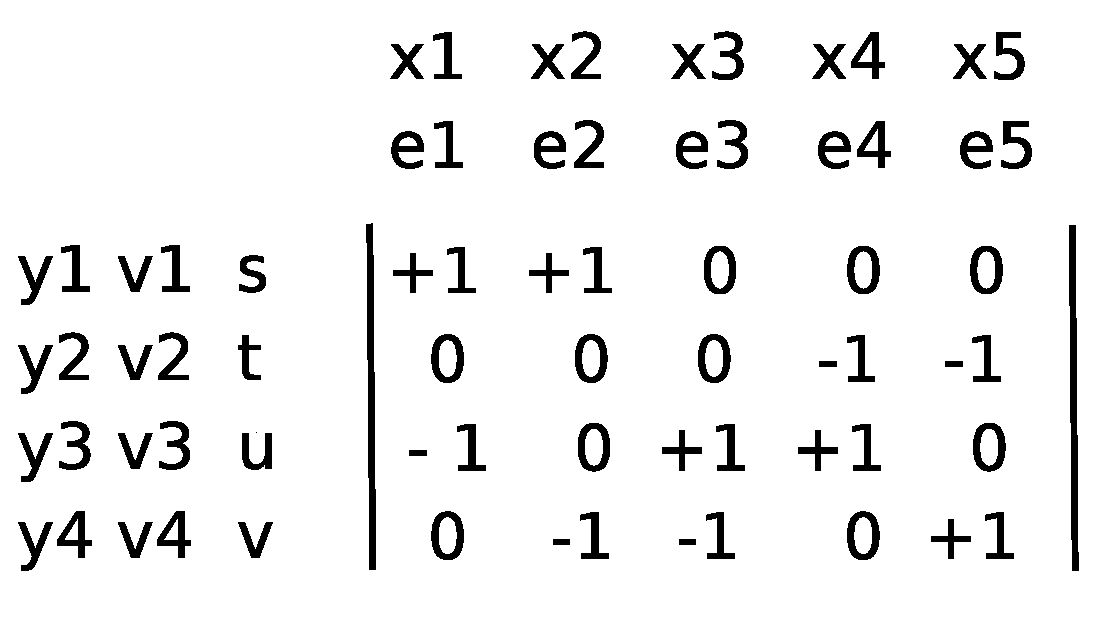
\includegraphics[width=1.8in] {L9-networkflowmatrix.eps}
%\end{figure}
%Node-arc matrix: $+1$ and $-1$ denote "start vertex" and "end vertex" of an edge, respectively.  
%} 


\frame{
\frametitle{Duality explanation of {\sc MaxFlow-MinCut}: Dual problem}

\begin{figure}
\begin{tikzpicture}[scale=0.8, auto,swap]
    % Draw a 7,11 network
    % First we draw the vertices
    \foreach \pos/\name in {{(0,0)/s}, {(2,1)/u}, {(2,-1)/v},
                            {(4,0)/t}}
        \node[middlevertex, draw,  fill=blue!20] (\name) at \pos {$\name$};
    % Connect vertices with edges and draw weights
    \foreach \source/ \dest /\weight in {u/v/{x_{3} },s/v/{x_{2} },   v/t/{x_{5} }}
        \path[edge] (\source) -- node[weight] {$\weight$} (\dest);
     \foreach \source/ \dest /\weight in {s/u/{x_{1} }, u/t/{x_{4} }} 
             \path[edge] (\source) -- node[weight, above] {$\weight$} (\dest);       
   \end{tikzpicture}
\end{figure}


{\sc Dual}: set variables for \textcolor{red}{edges}. Here $x_i$ denotes $flow$ via edge $i$. 
\begin{small}
\[
\begin{array}{rrrrrrrl}
 \max &         &            &          &            &           &    f   &\\
 s.t.     & x_1  & +x_2 &           &            &           &-f   & = 0   \text{ vertex } s\\
        &        &             &           &    -x_4 & -x_5 &+f & = 0  \text{ vertex } t\\
        & -x_1&            & +x_3 &+x_4   &         &      & = 0  \text{ vertex } u\\
        &         &-x_2    & -x_3   &            &+x_5 &     & = 0  \text{ vertex } v\\
        & x_1  &           &            &            &          &     & \leq C_1 \\
        &   &   x_2        &            &            &          &     & \leq C_2 \\
        &        &           &  x_{3}          &            &          &     & \leq C_3 \\
        &        &           &            &      x_{4}      &          &     & \leq C_4 \\
        &        &           &            &            &   x_{5}       &     & \leq C_5 \\
        & x_1,  &  x_{2},         &   x_{3},         &    x_{4},        &  x_{5}        &     & \geq 0 \\
\end{array} \nonumber
\]
\end{small}
} 

\frame{
\frametitle{An equivalent version} 
\begin{figure}
\begin{tikzpicture}[scale=0.8, auto,swap]
    % Draw a 7,11 network
    % First we draw the vertices
    \foreach \pos/\name in {{(0,0)/s}, {(2,1)/u}, {(2,-1)/v},
                            {(4,0)/t}}
        \node[middlevertex, draw,  fill=blue!20] (\name) at \pos {$\name$};
    % Connect vertices with edges and draw weights
    \foreach \source/ \dest /\weight in {u/v/{x_{3} },s/v/{x_{2} },   v/t/{x_{5} }}
        \path[edge] (\source) -- node[weight] {$\weight$} (\dest);
     \foreach \source/ \dest /\weight in {s/u/{x_{1} }, u/t/{x_{4} }} 
             \path[edge] (\source) -- node[weight, above] {$\weight$} (\dest);       
   \end{tikzpicture}
\end{figure}
\begin{small}
\[
\begin{array}{rrrrrrrl}
 \max &         &            &          &            &           &    f   &\\
 s.t.     & x_1  & +x_2 &           &            &           &-f   & \textcolor{red}{\leq} 0  \text{ vertex } s\\
        &        &             &           &    -x_4 & -x_5 &+f & \textcolor{red}{\leq} 0  \text{ vertex } t\\
        & -x_1&            & +x_3 &+x_4   &         &      & \textcolor{red}{\leq}0  \text{ vertex } u\\
        &         &-x_2    & -x_3   &            &+x_5 &     & \textcolor{red}{\leq}0  \text{ vertex } v\\
        & x_1  &           &            &            &          &     & \leq C_1 \\
        &   &   x_2        &            &            &          &     & \leq C_2 \\
        &        &           &  x_{3}          &            &          &     & \leq C_3 \\
        &        &           &            &      x_{4}      &          &     & \leq C_4 \\
        &        &           &            &            &   x_{5}       &     & \leq C_5 \\
        & x_1,  &  x_{2},         &   x_{3},         &    x_{4},        &  x_{5}        &     & \geq 0 \\
\end{array} \nonumber
\]
\end{small}
Note: The constraints (1), (2), (3), and (4) implies the equality $-x_{2} - x_{3} + x_{5} = 0$. So do the other equalities.   
} 


%\frame{
%	\frametitle{Totally unimodular matrix } 
%	\begin{definition}[Totally unimodular matrix]
%		A matrix $A$ is TUM iff all of its $k$-submatrix has 
%	\end{definition}
%}

\frame{
\frametitle{Duality explanation: Primal problem}

{\sc Primal}: set variables for \textcolor{red}{nodes}. 
\begin{footnotesize}
\[
\begin{array}{rrrrrrrrrrrrrrrrr}
 \min &       &   &   &   &  C_{1} z_1 & +C_{2} z_2   & +C_{3} z_3 & +C_{4} z_4& +C_{5}z_5 & \\
  s.t. & y_s &    &-y_u &            &+z_1  &  &  &  & & \geq 0\\
        & y_s &   &         & -y_v    &           &+z_2  &  &  & & \geq 0\\
        &        &   &  y_u & -y_v    &           &           &+z_3 &  & & \geq 0\\
        &        & -y_t  &  +y_u &        &           &           &      & +z_4 & & \geq 0\\
        &        & -y_t  &              &  +y_v      &           &           &      &     &  +z_5 & \geq 0\\
       & -y_s & +y_t  &              &         &           &           &      &     &    & \geq 1\\
      & y_s, & y_t,  & y_u,  & y_v,  &  z_1,  &  z_2,   &  z_3, &  z_4,& z_5 & \geq 0
\end{array} \nonumber
\]
\end{footnotesize}
Note: 
\begin{enumerate}
\item Since the constraints involves the difference among $y_{s}, y_{u}, y_{v}$ and $y_{t}$, one of them can be fixed without effects. Here, we fix $y_{s} = 0$. Thus we have $y_{t} \geq 1$ (by the constraint $-y_{s} + y_{t} \geq 1$). 
%\item Constraint (1) forces $z_{1} \geq y_{u}$ and the objective is to minimize $C_{1}z_{1}+...$, implying $z_{1} = y_{u}$.  So do constraint (2), and (3). 
\item Constraint (4) requires $z_{4} \geq y_{t} - y_{u}$, and the objective is to minimize a function containing $C_{4}z_{4}$, forcing $y_{t} = 1$. 
\item Constraint (1) requires $z_{1} \geq y_{u}$, and the objective is to minimize a function containing $C_{1}z_{1}$, forcing $z_{1} = y_{u}$. So does constraint (2).
\end{enumerate}

} 

\frame{
\frametitle{An equivalent LP model} 

{\sc Primal}: set variables for \textcolor{red}{nodes}. 
\begin{footnotesize}
\[
\begin{array}{rrrrrrrrrrrrrrrrr}
 \min &       &   &   &   &  C_{1} z_1 & +C_{2} z_2   & +C_{3} z_3 & +C_{4} z_4& +C_{5}z_5 & \\
  s.t. &     &    &-y_u &            &+z_1  &  &  &  & & \textcolor{red}{= 0}\\
        &      &   &         & -y_v    &           &+z_2  &  &  & &  \textcolor{red}{= 0}\\
        &        &   &  y_u & -y_v    &           &           &+z_3 &  & &  \geq 0\\
        &        &    &   y_u &        &           &           &      & +z_4 & &  \geq \textcolor{red}{1}\\
        &        &   &              &   y_v      &           &           &      &     &  +z_5 &  \geq \textcolor{red}{1}\\
       & y_s &    &              &         &           &           &      &     &    & \textcolor{red}{= 0}\\
       &       &   y_t  &              &         &           &           &      &     &    & \textcolor{red}{= 1}\\
      &       & & y_u,  & y_v,  &  z_1,  &  z_2,   &  z_3, &  z_4,& z_5 & \geq 0
\end{array} \nonumber
\]
\end{footnotesize}
Note: the coefficient matrix of constraints (3), (4) and (5) is totally uni-modular, implying the optimal solution is an integer solution. 
} 


\frame{
\frametitle{An equivalent ILP model} 

{\sc Primal}: set variables for \textcolor{red}{nodes}. 
\begin{footnotesize}
\[
\begin{array}{rrrrrrrrrrrrrrrrr}
 \min &       &   &   &   &  C_{1} z_1 & +C_{2} z_2   & +C_{3} z_3 & +C_{4} z_4& +C_{5}z_5 & \\
  s.t. &     &    &-y_u &            &+z_1  &  &  &  & & \textcolor{red}{= 0}\\
        &      &   &         & -y_v    &           &+z_2  &  &  & &  \textcolor{red}{= 0}\\
        &        &   &  y_u & -y_v    &           &           &+z_3 &  & &  \geq 0\\
        &        &    &   y_u &        &           &           &      & +z_4 & &  \geq \textcolor{red}{1}\\
        &        &   &              &   y_v      &           &           &      &     &  +z_5 &  \geq \textcolor{red}{1}\\
       & y_s &    &              &         &           &           &      &     &    & \textcolor{red}{= 0}\\
       &       &   y_t  &              &         &           &           &      &     &    & \textcolor{red}{= 1}\\
      &       & & y_u,  & y_v,  &  z_1,  &  z_2,   &  z_3, &  z_4,& z_5 & \textcolor{red}{= 0/1}
\end{array} \nonumber
\]
\end{footnotesize}

} 


\frame{
\frametitle{{\sc MaxFlow-MinCut}: strong duality} 

\begin{footnotesize}
\[
\begin{array}{rrrrrrrrrrrrrrrrr}
 \min &       &   &   &   &  C_{1} z_1 & +C_{2} z_2   & +C_{3} z_3 & +C_{4} z_4& +C_{5}z_5 & \\
  s.t. &     &    &-y_u &            &+z_1  &  &  &  & & \textcolor{red}{= 0}\\
        &      &   &         & -y_v    &           &+z_2  &  &  & &  \textcolor{red}{= 0}\\
        &        &   &  y_u & -y_v    &           &           &+z_3 &  & &  \geq 0\\
        &        &    &   y_u &        &           &           &      & +z_4 & &  \geq \textcolor{red}{1}\\
        &        &   &              &   y_v      &           &           &      &     &  +z_5 &  \geq \textcolor{red}{1}\\
       & y_s &    &              &         &           &           &      &     &    & \textcolor{red}{= 0}\\
       &       &   y_t  &              &         &           &           &      &     &    & \textcolor{red}{= 1}\\
      &       & & y_u,  & y_v,  &  z_1,  &  z_2,   &  z_3, &  z_4,& z_5 & \textcolor{red}{= 0/1}
\end{array} \nonumber
\]
\end{footnotesize}


\begin{itemize}
\item Suppose we explain the primal variables as:  
	\begin{itemize}
		\item  $y_{i}$ represents whether node $i$ is in $S$ or $\bar{S}$: if node $i$ is in $S$, $y_i=0$, and $y_i=1$ otherwise.
		\item $z_{i}$ represents whether an edge is a cut edge: For example,  $z_1 = 1 $ iff $y_s = 0$ and $y_u = 1$, i.e., edge $(s,u)$ is a cut edge. 
	\end{itemize}
\item Thus the primal problem is essentially to find a minimum cut. 
 \item By weak duality, we have $f\leq c$ and strong duality is exactly equivalent to the {\sc MaximumFlow-MinimumCut} theorem.
\end{itemize}
}



\frame{
\begin{block}{}
{\sc {\sc Ford-Fulkerson}} algorithm is essentially a primal-dual algorithm
\end{block}

}

\frame{
	\frametitle{Primal-dual algorithm} 
	\begin{itemize}
		\item Recall that the generic primal-dual algorithm can be described as follows.

	  \begin{algorithmic}[1]
    \STATE Initialize $\bf{x}$ as a dual feasible solution; 
    \WHILE{{\tt TRUE}}
    \STATE Construct DRP corresponding to ${x}$;
    \STATE Let $\omega_{opt}$ be the optimal solution to DRP; 
    \IF{$\omega_{opt} = 0$ }
    \RETURN{${x}$}; 
    \ELSE
    \STATE Improve ${x}$ using the optimal solution to DRP; 
    \ENDIF
    \ENDWHILE
  \end{algorithmic}
	\item We will show that solving DRP is equivalent to finding an augmentation path in residual graph. 
	\end{itemize}

}



\frame[allowframebreaks]{
\frametitle{Dual problem and DRP } 

 \begin{figure}
\begin{tikzpicture}[scale=1, auto,swap]

    \def\dx{0};
    \def\dy{0};	

     \foreach \x/\y/\name in {0/0/s, 2/1/u, 2/-1/v, 4/0/t}
        \node[middlevertex, draw,  fill=blue!20] (\name) at (\x+\dx, \y+\dy) {$\name$};
        
        
    \foreach \source/ \dest /\weight in {s/u/{x_1/64}}
        \path[edge, sloped, midway, above, allow upside down, black] (\source) -- node[weight] {\small $\weight$} (\dest);
        
    \foreach \source/ \dest /\weight in {u/t/{x_4/64}}
        \path[edge, sloped, midway, above, allow upside down] (\source) -- node[weight] {\small $\weight$} (\dest);        
        
    \foreach \source/ \dest /\weight in {u/v/{x_3/1}}
        \path[edge, sloped, midway, above, allow upside down, black] (\source) -- node[weight] {\small $\weight$} (\dest);
        
    \foreach \source/ \dest /\weight in {v/t/{x_5/32}}
        \path[edge, sloped, midway, below, allow upside down, black] (\source) -- node[weight] {\small $\weight$} (\dest);

    \foreach \source/ \dest /\weight in {s/v/{x_2/32}}
        \path[edge, sloped, midway, below, allow upside down] (\source) -- node[weight] {\small $\weight$} (\dest);
 %      \node[ultra thick, red, below] at (v.south) {Flow $f: $ $|f|=0$};          
        
        
%    \def\dx{5};
%    \def\dy{0};	
%
%     \foreach \x/\y/\name in {0/0/s, 2/1/u, 2/-1/v, 4/0/t}
%        \node[middlevertex, draw,  fill=blue!20] (\name) at (\x+\dx, \y+\dy) {$\name$};
%        
%%        \draw[->, thick] (s.15) -- node[below, sloped, midway] {\small $0$} (u.225);
%%        \draw[->, thick] (u.195) -- node[above, sloped, midway] {\small $1$} (s.45);
%%
%%        \draw[->, thick] (u.285) -- node[above, sloped, midway] {\small $0$} (v.75);
%%        \draw[->, thick, green] (v.105) -- node[above, sloped, midway, green] {\small $1$} (u.255);
%%
%%        \draw[->, thick] (v.15) -- node[below, sloped, midway] {\small $0$} (t.225);
%%        \draw[->, thick] (t.195) -- node[above, sloped, midway] {\small $1$} (v.45);
%
%        
%    \foreach \source/ \dest /\weight in {s/u/{64}}
%        \path[edge, sloped, midway, above, allow upside down, green] (\source) -- node[weight] {\small $\weight$} (\dest);
%        
%    \foreach \source/ \dest /\weight in {u/t/{64}}
%        \path[edge, sloped, midway, above, allow upside down] (\source) -- node[weight] {\small $\weight$} (\dest);        
%        
%    \foreach \source/ \dest /\weight in {u/v/{1}}
%        \path[edge, sloped, midway, above, allow upside down, green] (\source) -- node[weight] {\small $\weight$} (\dest);
%        
%    \foreach \source/ \dest /\weight in {v/t/{32}}
%        \path[edge, sloped, midway, below, allow upside down, green] (\source) -- node[weight] {\small $\weight$} (\dest);
%
%    \foreach \source/ \dest /\weight in {s/v/{32}}
%        \path[edge, sloped, midway, below, allow upside down] (\source) -- node[weight] {\small $\weight$} (\dest);
%       
%   \node[ultra thick, green, below] at (v.south) {An $s-t$ path in $G_f$};     
        
   \end{tikzpicture}
\end{figure}



\begin{itemize}
\item 
{\sc Dual D}: set variables for \textcolor{red}{edges};
% (Intuition: $x_i$ denotes $flow$ via edge $i$)
\begin{small}
\[
\begin{array}{rrrrrrrl}
 \max &         &            &          &            &           &    f   &\\
 s.t.     & x_1  & +x_2 &           &            &           &-f   & \textcolor{red}{\leq} 0  \text{ vertex } s\\
        &        &             &           &    -x_4 & -x_5 &+f & \textcolor{red}{\leq} 0  \text{ vertex } t\\
        & -x_1&            & +x_3 &+x_4   &         &      & \textcolor{red}{\leq}0  \text{ vertex } u\\
        &         &-x_2    & -x_3   &            &+x_5 &     & \textcolor{red}{\leq}0  \text{ vertex } v\\
        & x_1  &           &            &            &          &     & \leq 64 \\
        &   &   x_2        &            &            &          &     & \leq 32 \\
        &        &           &  x_{3}          &            &          &     & \leq 1 \\
        &        &           &            &      x_{4}      &          &     & \leq  64 \\
        &        &           &            &            &   x_{5}       &     & \leq 32 \\
        & x_1,  &  x_{2},         &   x_{3},         &    x_{4},        &  x_{5}        &     & \geq 0 \\
\end{array} \nonumber
\]
\end{small}


 \begin{figure}
\begin{tikzpicture}[scale=1, auto,swap]

    \def\dx{0};
    \def\dy{0};	

     \foreach \x/\y/\name in {0/0/s, 2/1/u, 2/-1/v, 4/0/t}
        \node[middlevertex, draw,  fill=blue!20] (\name) at (\x+\dx, \y+\dy) {$\name$};
        
        
    \foreach \source/ \dest /\weight in {s/u/{1/64}}
        \path[edge, sloped, midway, above, allow upside down, black] (\source) -- node[weight] {\small $\weight$} (\dest);
        
    \foreach \source/ \dest /\weight in {u/t/{0/64}}
        \path[edge, sloped, midway, above, allow upside down] (\source) -- node[weight] {\small $\weight$} (\dest);        
        
    \foreach \source/ \dest /\weight in {u/v/{1/1}}
        \path[edge, sloped, midway, above, allow upside down, black] (\source) -- node[weight] {\small $\weight$} (\dest);
        
    \foreach \source/ \dest /\weight in {v/t/{1/32}}
        \path[edge, sloped, midway, below, allow upside down, black] (\source) -- node[weight] {\small $\weight$} (\dest);

    \foreach \source/ \dest /\weight in {s/v/{0/32}}
        \path[edge, sloped, midway, below, allow upside down] (\source) -- node[weight] {\small $\weight$} (\dest);
 %      \node[ultra thick, red, below] at (v.south) {Flow $f: $ $|f|=0$};          
        
        
%    \def\dx{5};
%    \def\dy{0};	
%
%     \foreach \x/\y/\name in {0/0/s, 2/1/u, 2/-1/v, 4/0/t}
%        \node[middlevertex, draw,  fill=blue!20] (\name) at (\x+\dx, \y+\dy) {$\name$};
%        
%%        \draw[->, thick] (s.15) -- node[below, sloped, midway] {\small $0$} (u.225);
%%        \draw[->, thick] (u.195) -- node[above, sloped, midway] {\small $1$} (s.45);
%%
%%        \draw[->, thick] (u.285) -- node[above, sloped, midway] {\small $0$} (v.75);
%%        \draw[->, thick, green] (v.105) -- node[above, sloped, midway, green] {\small $1$} (u.255);
%%
%%        \draw[->, thick] (v.15) -- node[below, sloped, midway] {\small $0$} (t.225);
%%        \draw[->, thick] (t.195) -- node[above, sloped, midway] {\small $1$} (v.45);
%
%        
%    \foreach \source/ \dest /\weight in {s/u/{64}}
%        \path[edge, sloped, midway, above, allow upside down, green] (\source) -- node[weight] {\small $\weight$} (\dest);
%        
%    \foreach \source/ \dest /\weight in {u/t/{64}}
%        \path[edge, sloped, midway, above, allow upside down] (\source) -- node[weight] {\small $\weight$} (\dest);        
%        
%    \foreach \source/ \dest /\weight in {u/v/{1}}
%        \path[edge, sloped, midway, above, allow upside down, green] (\source) -- node[weight] {\small $\weight$} (\dest);
%        
%    \foreach \source/ \dest /\weight in {v/t/{32}}
%        \path[edge, sloped, midway, below, allow upside down, green] (\source) -- node[weight] {\small $\weight$} (\dest);
%
%    \foreach \source/ \dest /\weight in {s/v/{32}}
%        \path[edge, sloped, midway, below, allow upside down] (\source) -- node[weight] {\small $\weight$} (\dest);
%       
%   \node[ultra thick, green, below] at (v.south) {An $s-t$ path in $G_f$};     
        
   \end{tikzpicture}
\end{figure}
\item Let's consider a dual feasible solution ${x}=(1, 0, 1, 0, 1)$. Recall how to write $DRP$ from $D$:
	\begin{itemize}
		\item Replacing the right-hand side $C_i$ with $0$; 
		\item Adding constraints: $x_i\leq 1$,  $f\leq 1$; 
		\item Keep only the tight constraints $J$. Here we category $J$ into two sets, i.e. $J = J^S \cup J^E$, where $J^S$ records the saturated arcs $J^S=\{i | x_i = C_i \}$, and $J^E$ records the empty arcs $J^E=\{i | x_i = 0 \}$. In the above example, $J_S=\{3\}$, and $J_E=\{2, 4\}$. 
		
	\end{itemize}
\end{itemize}
} 


\frame{
\frametitle{$DRP$ corresponds to finding an augmentation path} 

\begin{itemize}
\item 
\begin{footnotesize}
DRP: 
\[
\begin{array}{rrrrrrrl}
 \max &         &            &          &            &           &    f   &\\
 s.t.     & x_1  & +x_2 &           &            &           &-f   & = 0   \text{ vertex } s\\
        &        &             &           &    -x_4 & -x_5 &+f & = 0  \text{ vertex } t\\
        & -x_1&            & +x_3 &+x_4   &         &      & = 0  \text{ vertex } u\\
        &         &-x_2    & -x_3   &            &+x_5 &     & = 0  \text{ vertex } v\\
        &   &           &        x_{i}    &            &          &     &  \textcolor{blue}\leq 0 \text{\quad}  i \in J^S \\
        &   &           &        x_{j}    &            &          &     &  \textcolor{red}\geq 0 \text{\quad}   j \in J^E \\
        & x_1,  &  x_{2},         &   x_{3},         &    x_{4},        &  x_{5},        &  f   & \textcolor{black}{\leq 1} 
\end{array} 
\]
\end{footnotesize}
\begin{small}
 \item $\omega_{OPT} = 0$ implies that optimal solution is found. In contrast, $\omega_{OPT} = 1$ implies an augmentation $s-t$ path (with unit flow) in $G_f$. 
 \end{small}
\end{itemize}
 \begin{figure}
\begin{tikzpicture}[scale=0.85, auto,swap]

    \def\dx{0};
    \def\dy{0};	

     \foreach \x/\y/\name in {0/0/s, 2/1/u, 2/-1/v, 4/0/t}
        \node[middlevertex, draw,  fill=blue!20] (\name) at (\x+\dx, \y+\dy) {$\name$};
        
        
    \foreach \source/ \dest /\weight in {s/u/{x_1}}
        \path[edge, sloped, midway, above, allow upside down, black] (\source) -- node[weight] {\footnotesize $\weight$} (\dest);
        
    \foreach \source/ \dest /\weight in {u/t/\textcolor{red}{x_4\geq0}}
        \path[edge, sloped, midway, above, allow upside down] (\source) -- node[weight] {\footnotesize $\weight$} (\dest);        
        
    \foreach \source/ \dest /\weight in {u/v/\textcolor{blue}{x_3\leq0}}
        \path[edge, sloped, midway, above, allow upside down, black] (\source) -- node[weight] {\footnotesize $\weight$} (\dest);
        
    \foreach \source/ \dest /\weight in {v/t/{x_5}}
        \path[edge, sloped, midway, below, allow upside down, black] (\source) -- node[weight] {\footnotesize $\weight$} (\dest);

    \foreach \source/ \dest /\weight in {s/v/\textcolor{red}{x_2\geq0}}
        \path[edge, sloped, midway, below, allow upside down] (\source) -- node[weight] {\footnotesize $\weight$} (\dest);
       \node[ultra thick, red, below] at (v.south) {DRP};          
        
        
    \def\dx{6};
    \def\dy{0};	

     \foreach \x/\y/\name in {0/0/s, 2/1/u, 2/-1/v, 4/0/t}
        \node[middlevertex, draw,  fill=blue!20] (\name) at (\x+\dx, \y+\dy) {$\name$};
        
        \draw[->, thick] (s.15) -- node[below, sloped, midway] {\footnotesize $63$} (u.225);
        \draw[->, thick] (u.195) -- node[above, sloped, midway] {\footnotesize $1$} (s.45);

        \draw[->, thick] (u.285) -- node[above, sloped, midway] {\footnotesize $0$} (v.75);
        \draw[->, thick] (v.105) -- node[above, sloped, midway] {\footnotesize $1$} (u.255);

        \draw[->, thick] (v.15) -- node[below, sloped, midway] {\footnotesize $31$} (t.225);
        \draw[->, thick] (t.195) -- node[above, sloped, midway] {\footnotesize $1$} (v.45);

        
%    \foreach \source/ \dest /\weight in {s/u/{0/64}}
%        \path[edge, sloped, midway, above, allow upside down, blue] (\source) -- node[weight] {\small $\weight$} (\dest);
%        
    \foreach \source/ \dest /\weight in {u/t/{64}}
        \path[edge, sloped, midway, above, allow upside down] (\source) -- node[weight] {\footnotesize $\weight$} (\dest);        
        
%    \foreach \source/ \dest /\weight in {u/v/{0/1}}
%        \path[edge, sloped, midway, above, allow upside down, blue] (\source) -- node[weight] {\small $\weight$} (\dest);
%        
%    \foreach \source/ \dest /\weight in {v/t/{0/32}}
%        \path[edge, sloped, midway, below, allow upside down, blue] (\source) -- node[weight] {\small $\weight$} (\dest);

    \foreach \source/ \dest /\weight in {s/v/{32}}
        \path[edge, sloped, midway, below, allow upside down] (\source) -- node[weight] {\footnotesize $\weight$} (\dest);
       
   \node[ultra thick, below, green] at (v.south) {Residual graph $G_f$};     
        
   \end{tikzpicture}
\end{figure}
}

\frame{
\frametitle{DRP and augmentation path in residual graph}

 \begin{figure}
\begin{tikzpicture}[scale=1, auto,swap]

    \def\dx{0};
    \def\dy{0};	

     \foreach \x/\y/\name in {0/0/s, 2/1/u, 2/-1/v, 4/0/t}
        \node[middlevertex, draw,  fill=blue!20] (\name) at (\x+\dx, \y+\dy) {$\name$};
        
        
    \foreach \source/ \dest /\weight in {s/u/{x_1}}
        \path[edge, sloped, midway, above, allow upside down, black] (\source) -- node[weight] {\small $\weight$} (\dest);
        
    \foreach \source/ \dest /\weight in {u/t/\textcolor{red}{x_4\geq0}}
        \path[edge, sloped, midway, above, allow upside down] (\source) -- node[weight] {\small $\weight$} (\dest);        
        
    \foreach \source/ \dest /\weight in {u/v/\textcolor{blue}{x_3\leq0}}
        \path[edge, sloped, midway, above, allow upside down, black] (\source) -- node[weight] {\small $\weight$} (\dest);
        
    \foreach \source/ \dest /\weight in {v/t/{x_5}}
        \path[edge, sloped, midway, below, allow upside down, black] (\source) -- node[weight] {\small $\weight$} (\dest);

    \foreach \source/ \dest /\weight in {s/v/\textcolor{red}{x_2\geq0}}
        \path[edge, sloped, midway, below, allow upside down] (\source) -- node[weight] {\small $\weight$} (\dest);
       \node[ultra thick, red, below] at (v.south) {DRP};          
        
        
    \def\dx{6};
    \def\dy{0};	

     \foreach \x/\y/\name in {0/0/s, 2/1/u, 2/-1/v, 4/0/t}
        \node[middlevertex, draw,  fill=blue!20] (\name) at (\x+\dx, \y+\dy) {$\name$};
        
        \draw[->, thick] (s.15) -- node[below, sloped, midway] {\small $63$} (u.225);
        \draw[->, thick] (u.195) -- node[above, sloped, midway] {\small $1$} (s.45);

        \draw[->, thick] (u.285) -- node[above, sloped, midway] {\small $0$} (v.75);
        \draw[->, thick] (v.105) -- node[above, sloped, midway] {\small $1$} (u.255);

        \draw[->, thick] (v.15) -- node[below, sloped, midway] {\small $31$} (t.225);
        \draw[->, thick] (t.195) -- node[above, sloped, midway] {\small $1$} (v.45);

        
%    \foreach \source/ \dest /\weight in {s/u/{0/64}}
%        \path[edge, sloped, midway, above, allow upside down, blue] (\source) -- node[weight] {\small $\weight$} (\dest);
%        
    \foreach \source/ \dest /\weight in {u/t/{64}}
        \path[edge, sloped, midway, above, allow upside down] (\source) -- node[weight] {\small $\weight$} (\dest);        
        
%    \foreach \source/ \dest /\weight in {u/v/{0/1}}
%        \path[edge, sloped, midway, above, allow upside down, blue] (\source) -- node[weight] {\small $\weight$} (\dest);
%        
%    \foreach \source/ \dest /\weight in {v/t/{0/32}}
%        \path[edge, sloped, midway, below, allow upside down, blue] (\source) -- node[weight] {\small $\weight$} (\dest);

    \foreach \source/ \dest /\weight in {s/v/{32}}
        \path[edge, sloped, midway, below, allow upside down] (\source) -- node[weight] {\small $\weight$} (\dest);
       
   \node[ultra thick, below, green] at (v.south) {Residual graph $G_f$};     
        
   \end{tikzpicture}
\end{figure}
\begin{itemize}

\item Note that DRP corresponds to finding an augmentation path in the residual graph $G_f$.
	\begin{itemize}
		\item $x_{i}  \leq 0,  i \in J^S$, e.g., $x_{3}$,  denotes a backward edge.   
		\item $x_{j}  \geq 0,  j \in J^E$, e.g., $x_{2}$,  denotes a forward edge, 
		\item and for other edges, there is no restriction for $x_i$, e.g., $x_{1}$. 
	\end{itemize}
\item Thus {\sc {\sc Ford-Fulkerson}} algorithm is essentially a primal-dual algorithm.

\end{itemize}

}


\frame{
\begin{block}{}
 {\sc {\sc Ford-Fulkerson}} algorithm: bad example 1
 \end{block}
}


\frame{
	\frametitle{The integer restriction is important} 
	\begin{itemize}
	\item In the analysis of {\sc {\sc Ford-Fulkerson}}  algorithm, the integer restriction of capacities is important: the bottleneck edge leads to an increase of at least $1$. 
	\item The analysis doesn't hold if the capacities can be irrational. 
	 In fact, the flow might be increased by a smaller and smaller number and the iteration will be endless. 
	 Worse yet, this endless iteration might not converge to the maximum flow. 
	\end{itemize}
(See an example by Uri Zwick)
} 

\frame{
\begin{block}{}
 {\sc {\sc Ford-Fulkerson}} algorithm: bad example 2
 \end{block}
 
 \begin{figure}
\begin{tikzpicture}[scale=1.3, auto,swap]
    % Draw a 7,11 network
    % First we draw the vertices
    \foreach \pos/\name in {{(0,0)/s}, {(2,1)/u}, {(2,-1)/v},
                            {(4,0)/t}}
        \node[middlevertex, draw,  fill=blue!20] (\name) at \pos {$\name$};
    % Connect vertices with edges and draw weights
    \foreach \source/ \dest /\weight in {s/u/{c_1=64}, u/t/{c_4=64},u/v/{c_3=1},s/v/{c_2=32},      v/t/{c_5=32} }
        \path[edge, sloped, midway, below, allow upside down] (\source) -- node[weight] {$\weight$} (\dest);
   \end{tikzpicture}
\end{figure}


}


\frame{
\frametitle{A bad example of  {\sc {\sc Ford-Fulkerson}} algorithm: Step 1 } 

 \begin{figure}
\begin{tikzpicture}[scale=1, auto,swap]

    \def\dx{0};
    \def\dy{0};	

     \foreach \x/\y/\name in {0/0/s, 2/1/u, 2/-1/v, 4/0/t}
        \node[middlevertex, draw,  fill=blue!20] (\name) at (\x+\dx, \y+\dy) {$\name$};
        
        
    \foreach \source/ \dest /\weight in {s/u/{0/64}}
        \path[edge, sloped, midway, above, allow upside down, black] (\source) -- node[weight] {\small $\weight$} (\dest);
        
    \foreach \source/ \dest /\weight in {u/t/{0/64}}
        \path[edge, sloped, midway, above, allow upside down] (\source) -- node[weight] {\small $\weight$} (\dest);        
        
    \foreach \source/ \dest /\weight in {u/v/{0/1}}
        \path[edge, sloped, midway, above, allow upside down, black] (\source) -- node[weight] {\small $\weight$} (\dest);
        
    \foreach \source/ \dest /\weight in {v/t/{0/32}}
        \path[edge, sloped, midway, below, allow upside down, black] (\source) -- node[weight] {\small $\weight$} (\dest);

    \foreach \source/ \dest /\weight in {s/v/{0/32}}
        \path[edge, sloped, midway, below, allow upside down] (\source) -- node[weight] {\small $\weight$} (\dest);
       \node[ultra thick, red, below] at (v.south) {Flow $f: $ $|f|=0$};          
        
        
    \def\dx{5};
    \def\dy{0};	

     \foreach \x/\y/\name in {0/0/s, 2/1/u, 2/-1/v, 4/0/t}
        \node[middlevertex, draw,  fill=blue!20] (\name) at (\x+\dx, \y+\dy) {$\name$};
        
%        \draw[->, thick] (s.15) -- node[below, sloped, midway] {\small $0$} (u.225);
%        \draw[->, thick] (u.195) -- node[above, sloped, midway] {\small $1$} (s.45);
%
%        \draw[->, thick] (u.285) -- node[above, sloped, midway] {\small $0$} (v.75);
%        \draw[->, thick, green] (v.105) -- node[above, sloped, midway, green] {\small $1$} (u.255);
%
%        \draw[->, thick] (v.15) -- node[below, sloped, midway] {\small $0$} (t.225);
%        \draw[->, thick] (t.195) -- node[above, sloped, midway] {\small $1$} (v.45);

        
    \foreach \source/ \dest /\weight in {s/u/{64}}
        \path[edge, sloped, midway, above, allow upside down, green] (\source) -- node[weight] {\small $\weight$} (\dest);
        
    \foreach \source/ \dest /\weight in {u/t/{64}}
        \path[edge, sloped, midway, above, allow upside down] (\source) -- node[weight] {\small $\weight$} (\dest);        
        
    \foreach \source/ \dest /\weight in {u/v/{1}}
        \path[edge, sloped, midway, above, allow upside down, green] (\source) -- node[weight] {\small $\weight$} (\dest);
        
    \foreach \source/ \dest /\weight in {v/t/{32}}
        \path[edge, sloped, midway, below, allow upside down, green] (\source) -- node[weight] {\small $\weight$} (\dest);

    \foreach \source/ \dest /\weight in {s/v/{32}}
        \path[edge, sloped, midway, below, allow upside down] (\source) -- node[weight] {\small $\weight$} (\dest);
       
   \node[ultra thick, green, below] at (v.south) {An $s-t$ path in $G_f$};     
        
   \end{tikzpicture}
\end{figure}




%\begin{figure}
% \includegraphics[width=3in] {L10-networkflowFFstep1.eps}
%\end{figure}
}

\frame{
\frametitle{A bad example of  {\sc {\sc Ford-Fulkerson}} algorithm: Step 2 } 

 \begin{figure}
\begin{tikzpicture}[scale=1, auto,swap]

    \def\dx{0};
    \def\dy{0};	

     \foreach \x/\y/\name in {0/0/s, 2/1/u, 2/-1/v, 4/0/t}
        \node[middlevertex, draw,  fill=blue!20] (\name) at (\x+\dx, \y+\dy) {$\name$};
        
        
    \foreach \source/ \dest /\weight in {s/u/{1/64}}
        \path[edge, sloped, midway, above, allow upside down, black] (\source) -- node[weight] {\small $\weight$} (\dest);
        
    \foreach \source/ \dest /\weight in {u/t/{0/64}}
        \path[edge, sloped, midway, above, allow upside down] (\source) -- node[weight] {\small $\weight$} (\dest);        
        
    \foreach \source/ \dest /\weight in {u/v/{1/1}}
        \path[edge, sloped, midway, above, allow upside down, black] (\source) -- node[weight] {\small $\weight$} (\dest);
        
    \foreach \source/ \dest /\weight in {v/t/{1/32}}
        \path[edge, sloped, midway, below, allow upside down, black] (\source) -- node[weight] {\small $\weight$} (\dest);

    \foreach \source/ \dest /\weight in {s/v/{0/32}}
        \path[edge, sloped, midway, below, allow upside down] (\source) -- node[weight] {\small $\weight$} (\dest);
       \node[ultra thick, red, below] at (v.south) {Flow $f: $ $|f|=1$};          
        
        
    \def\dx{5};
    \def\dy{0};	

     \foreach \x/\y/\name in {0/0/s, 2/1/u, 2/-1/v, 4/0/t}
        \node[middlevertex, draw,  fill=blue!20] (\name) at (\x+\dx, \y+\dy) {$\name$};
        
        \draw[->, thick] (s.15) -- node[below, sloped, midway] {\small $63$} (u.225);
        \draw[->, thick] (u.195) -- node[above, sloped, midway] {\small $1$} (s.45);

        \draw[->, thick] (u.285) -- node[above, sloped, midway] {\small $0$} (v.75);
        \draw[->, thick, green] (v.105) -- node[above, sloped, midway, green] {\small $1$} (u.255);

        \draw[->, thick] (v.15) -- node[below, sloped, midway] {\small $31$} (t.225);
        \draw[->, thick] (t.195) -- node[above, sloped, midway] {\small $1$} (v.45);

        
%    \foreach \source/ \dest /\weight in {s/u/{0/64}}
%        \path[edge, sloped, midway, above, allow upside down, blue] (\source) -- node[weight] {\small $\weight$} (\dest);
%        
    \foreach \source/ \dest /\weight in {u/t/{64}}
        \path[edge, sloped, midway, above, allow upside down, green] (\source) -- node[weight] {\small $\weight$} (\dest);        
        
%    \foreach \source/ \dest /\weight in {u/v/{0/1}}
%        \path[edge, sloped, midway, above, allow upside down, blue] (\source) -- node[weight] {\small $\weight$} (\dest);
%        
%    \foreach \source/ \dest /\weight in {v/t/{0/32}}
%        \path[edge, sloped, midway, below, allow upside down, blue] (\source) -- node[weight] {\small $\weight$} (\dest);

    \foreach \source/ \dest /\weight in {s/v/{32}}
        \path[edge, sloped, midway, below, allow upside down, green] (\source) -- node[weight] {\small $\weight$} (\dest);
       
   \node[ultra thick, below, green] at (v.south) {An $s-t$ path in $G_f$};     
        
   \end{tikzpicture}
\end{figure}


%\begin{figure}
% \includegraphics[width=3in] {L10-networkflowFFstep2.eps}
%\end{figure}
}


\frame{
\frametitle{A bad example of  {\sc {\sc Ford-Fulkerson}} algorithm: Step 3 } 
%\begin{figure}
% \includegraphics[width=3in] {L10-networkflowFFstep3.eps}
%\end{figure}

 \begin{figure}
\begin{tikzpicture}[scale=1, auto,swap]

    \def\dx{0};
    \def\dy{0};	

     \foreach \x/\y/\name in {0/0/s, 2/1/u, 2/-1/v, 4/0/t}
        \node[middlevertex, draw,  fill=blue!20] (\name) at (\x+\dx, \y+\dy) {$\name$};
        
        
    \foreach \source/ \dest /\weight in {s/u/{1/64}}
        \path[edge, sloped, midway, above, allow upside down, black] (\source) -- node[weight] {\small $\weight$} (\dest);
        
    \foreach \source/ \dest /\weight in {u/t/{1/64}}
        \path[edge, sloped, midway, above, allow upside down] (\source) -- node[weight] {\small $\weight$} (\dest);        
        
    \foreach \source/ \dest /\weight in {u/v/{0/1}}
        \path[edge, sloped, midway, above, allow upside down, black] (\source) -- node[weight] {\small $\weight$} (\dest);
        
    \foreach \source/ \dest /\weight in {v/t/{1/32}}
        \path[edge, sloped, midway, below, allow upside down, black] (\source) -- node[weight] {\small $\weight$} (\dest);

    \foreach \source/ \dest /\weight in {s/v/{1/32}}
        \path[edge, sloped, midway, below, allow upside down] (\source) -- node[weight] {\small $\weight$} (\dest);
        
       \node[ultra thick, red, below] at (v.south) {Flow $f: $ $|f|=2$};          
        
   \end{tikzpicture}
\end{figure}



\begin{itemize}
\item 
Note that after two iterations, the problem is similar to the original problem except for the capacities on $(s,u), (s,v), (u,t), (v,t)$ decrease by 1. 
\item 
Thus  {\sc {\sc Ford-Fulkerson}} algorithm will end after $64+32$ iterations as $bottleneck=1$ at all intermediate stages.
\end{itemize}
}


\frame{
	\frametitle{{\sc {\sc Ford-Fulkerson}} algorithm: weakness   }
	
	\begin{itemize}
		\item Arbitrary selection of augmentation paths will lead to the following weaknesses: 
			\begin{itemize}
				\item A path with small bottleneck capacity is chosen as augmentation path; 
				\item We put flow on too many edges than necessary. 
			\end{itemize}
		\item In the original paper by Ford and Fulkerson, several heuristics for improvement were examined. 
	\end{itemize}
}

%\frame{
%\begin{block}{}
%	Improvements of {\sc {\sc Ford-Fulkerson}} algorithm   
%\end{block} 
%} 




\frame{
\frametitle{Improvements of  {\sc {\sc Ford-Fulkerson}} algorithm  }
\begin{itemize} 
%not  FF, except for finding an augmentation path $P$, cost time proportional to the length of $P$, that is, $O(|P|)=O(|V|)$. (Indeed, all computations and updates are made along $P$, while the remainder of the data is not touched.) 
%\item However, the search  running on $G$ cost $O(|E|)$, which  is $O(|V|^{2)}$ in general case, substantially more than $O(|P|)$ or $O(|V|)$.  
\item Various strategies to select  augmentation path in $G_f$: 
\begin{enumerate}
\item Fat pipes: 
	\begin{itemize}
		\item To select the augmentation path with \textcolor{red}{\bf the largest bottleneck capacity}, or  find an augmentation  path with \textcolor{red}{\bf large}  improvement using \textcolor{red}{\bf scaling} technique. 
	\end{itemize}
\item Short pipes: 
	\begin{itemize}	
		\item {\sc {\sc Edmonds-Karp}} algorithm: find \textcolor{red}{\bf the shortest augmentation path}. 
		\item Dinitz' algorithm: extend \textcolor{blue}{\bf BFS tree} to \textcolor{red}{\bf layered network} to record all edges contained in shortest augmentation paths, find augmentation path in the layered network, and perform \textcolor{red}{\bf amortized analysis}.
		\item Dinic's algorithm: running \textcolor{red}{\bf DFS} in \textcolor{red}{\bf layered network} to find \textcolor{red}{\bf blocking flow} that saturate \textcolor{red}{\bf all shortest augmentation paths}. 
		\item Karzanov algorithm: unlike Dinitz' algorithm \textcolor{red}{\bf saturates edges} when constructing blocking flow, Karzanov's algorithm \textcolor{red}{\bf saturates nodes} using the \textcolor{red}{\bf pre-flow} idea.   
		\item {\sc Push-Relabel} algorithm:  The algorithm uses the idea of pre-flow; however, the pre-flow was not constructed in \textcolor{red}{\bf layered network} but in residual graph directly. \textcolor{red}{\bf Distance labels} were used  \textcolor{red}{\bf to estimate the shortest distance from  nodes to $t$}. 
	\end{itemize}
\end{enumerate}
%\item The complexity of {\sc {\sc Edmonds-Karp}} and {\sc Dinic's} algorithms do not depend on edge capacities, and thus avoid the limitation of {\sc Ford-Fulkerson} algorithm for the networks with irrational edge capacities.  
\end{itemize} 
} 


\frame{
\begin{block}{}
 Improvement 1: Scaling technique for  speed-up (by Y. Dinitz)
\end{block}
}


\frame{
\frametitle{Scaling technique  }


\begin{itemize}
\item Question: can we choose a  \textcolor{red}{\bf large} augmentation path? The larger $bottleneck(p,f)$ is, the less iterations are needed. 
\item 
An $s-t$ path $p$ in $G_f$ with the \textcolor{red}{\bf largest $bottleneck(p, f)$} can be found using binary search, or a slight change of Dijkstra's algorithm in $O(m+n\log n)$ time; however, it is still somewhat inefficient. 
%However, it is inefficient to find an $s-t$ path $p$ in $G_f$ with the \textcolor{red}{\bf largest $bottleneck(p, f)$}. (A slight change of Dijkstra's algorithm works here, taking $O(m+n \log n)$ time)
\item 
Basic idea: Let's relax the \textcolor{red}{\bf ``largest''} requirement to \textcolor{red}{\bf ``sufficiently large''}. 
  Specifically, we can set up a lower bound $\Delta$ for $bottleneck(P,f)$ by \textcolor{red}{\bf simply removing the ``small'' edges}, i.e.  the edges with capacities less than $\Delta$ from $G(f)$. This residual graph is called $G_{f}(\Delta)$ and  
$\Delta$ will be scaled down as iteration proceeds. 
\end{itemize}
}

\frame{
%\frametitle{{\sc Scaling {\sc Ford-Fulkerson}} algorithm }
\begin{itemize}
\item 
{\sc Scaling-{\sc Ford-Fulkerson}}$(G)$\\
  \begin{algorithmic}[1]
    \STATE Initialize $f(e)=0$ for all $e$.
    \STATE \textcolor{red}{Let $\Delta = C$;}
    \WHILE{\textcolor{red}{$\Delta \geq 1$}}  
    \WHILE{there is an $s-t$ path in \textcolor{red}{$G_f(\Delta)$}}
    \STATE Choose an $s-t$ path $p$; 
    \STATE $f = ${\sc augment}$(p,f)$;
    \ENDWHILE
    \STATE \textcolor{red}{$\Delta = \tfrac{\Delta}{2}$;}
    \ENDWHILE
    \RETURN{$f$};
  \end{algorithmic}


 \item 
Intuition: flow is augmented in a large step size whenever possible; otherwise, the step size is scaled down. Step size is controlled via removing the ``small'' edges out of residual graph.
\item 
Note that $\Delta$ turns to be  $1$ finally; thus no edge in residual graph will be neglected.
\end{itemize}
}


\frame{
\frametitle{An example: Step 1} 
%\begin{figure}
% \includegraphics[width=2in] {L10-networkflowscaling1.eps}
%\end{figure}


 \begin{figure}
\begin{tikzpicture}[scale=1, auto,swap]

    \def\dx{0};
    \def\dy{0};	

     \foreach \x/\y/\name in {0/0/s, 2/1/u, 2/-1/v, 4/0/t}
        \node[middlevertex, draw,  fill=blue!20] (\name) at (\x+\dx, \y+\dy) {$\name$};
        
        
    \foreach \source/ \dest /\weight in {s/u/{0/64}}
        \path[edge, sloped, midway, above, allow upside down, black] (\source) -- node[weight] {\small $\weight$} (\dest);
        
    \foreach \source/ \dest /\weight in {u/t/{0/64}}
        \path[edge, sloped, midway, above, allow upside down] (\source) -- node[weight] {\small $\weight$} (\dest);        
        
    \foreach \source/ \dest /\weight in {u/v/{0/1}}
        \path[edge, sloped, midway, above, allow upside down, black] (\source) -- node[weight] {\small $\weight$} (\dest);
        
    \foreach \source/ \dest /\weight in {v/t/{0/32}}
        \path[edge, sloped, midway, below, allow upside down, black] (\source) -- node[weight] {\small $\weight$} (\dest);

    \foreach \source/ \dest /\weight in {s/v/{0/32}}
        \path[edge, sloped, midway, below, allow upside down] (\source) -- node[weight] {\small $\weight$} (\dest);
       \node[ultra thick, red, below] at (v.south) {Flow $f: $ $|f|=0$};          
        
        
    \def\dx{5};
    \def\dy{0};	

     \foreach \x/\y/\name in {0/0/s, 2/1/u, 2/-1/v, 4/0/t}
        \node[middlevertex, draw,  fill=blue!20] (\name) at (\x+\dx, \y+\dy) {$\name$};
        
%        \draw[->, thick] (s.15) -- node[below, sloped, midway] {\small $0$} (u.225);
%        \draw[->, thick] (u.195) -- node[above, sloped, midway] {\small $1$} (s.45);
%
%        \draw[->, thick] (u.285) -- node[above, sloped, midway] {\small $0$} (v.75);
%        \draw[->, thick, green] (v.105) -- node[above, sloped, midway, green] {\small $1$} (u.255);
%
%        \draw[->, thick] (v.15) -- node[below, sloped, midway] {\small $0$} (t.225);
%        \draw[->, thick] (t.195) -- node[above, sloped, midway] {\small $1$} (v.45);

        
    \foreach \source/ \dest /\weight in {s/u/{64}}
        \path[edge, sloped, midway, above, allow upside down, gray] (\source) -- node[weight] {\small $\weight$} (\dest);
        
    \foreach \source/ \dest /\weight in {u/t/{64}}
        \path[edge, sloped, midway, above, allow upside down, gray] (\source) -- node[weight] {\small $\weight$} (\dest);        
        
    \foreach \source/ \dest /\weight in {u/v/{1}}
        \path[edge, sloped, midway, above, allow upside down, gray] (\source) -- node[weight] {\small $\weight$} (\dest);
        
    \foreach \source/ \dest /\weight in {v/t/{32}}
        \path[edge, sloped, midway, below, allow upside down, gray] (\source) -- node[weight] {\small $\weight$} (\dest);

    \foreach \source/ \dest /\weight in {s/v/{32}}
        \path[edge, sloped, midway, below, allow upside down, gray] (\source) -- node[weight] {\small $\weight$} (\dest);
       
   \node[ultra thick, green, below] at (v.south) {No $s-t$ path in $G_f$};     
        
   \end{tikzpicture}
\end{figure}



\begin{footnotesize}
\begin{itemize}
 \item Flow: 0 flow;
 \item $\Delta$: $\Delta = 96$;
 \item $G_f(\Delta)$: the edges in light blue  were removed since capcities are less than 96.
 \item $s-t$ path: cannot find. Thus $\Delta$ is scaled: $\Delta = \tfrac{\Delta}{2} = 48$.  
\end{itemize}
\end{footnotesize}
}

\frame{
\frametitle{An example: Step 2} 
%\begin{figure}
% \includegraphics[width=2in] {L10-networkflowscaling2.eps}
%\end{figure}


 \begin{figure}
\begin{tikzpicture}[scale=1, auto,swap]

    \def\dx{0};
    \def\dy{0};	

     \foreach \x/\y/\name in {0/0/s, 2/1/u, 2/-1/v, 4/0/t}
        \node[middlevertex, draw,  fill=blue!20] (\name) at (\x+\dx, \y+\dy) {$\name$};
        
        
    \foreach \source/ \dest /\weight in {s/u/{0/64}}
        \path[edge, sloped, midway, above, allow upside down, black] (\source) -- node[weight] {\small $\weight$} (\dest);
        
    \foreach \source/ \dest /\weight in {u/t/{0/64}}
        \path[edge, sloped, midway, above, allow upside down] (\source) -- node[weight] {\small $\weight$} (\dest);        
        
    \foreach \source/ \dest /\weight in {u/v/{0/1}}
        \path[edge, sloped, midway, above, allow upside down, black] (\source) -- node[weight] {\small $\weight$} (\dest);
        
    \foreach \source/ \dest /\weight in {v/t/{0/32}}
        \path[edge, sloped, midway, below, allow upside down, black] (\source) -- node[weight] {\small $\weight$} (\dest);

    \foreach \source/ \dest /\weight in {s/v/{0/32}}
        \path[edge, sloped, midway, below, allow upside down] (\source) -- node[weight] {\small $\weight$} (\dest);
       \node[ultra thick, red, below] at (v.south) {Flow $f: $ $|f|=0$};          
        
        
    \def\dx{5};
    \def\dy{0};	

     \foreach \x/\y/\name in {0/0/s, 2/1/u, 2/-1/v, 4/0/t}
        \node[middlevertex, draw,  fill=blue!20] (\name) at (\x+\dx, \y+\dy) {$\name$};
        
%        \draw[->, thick] (s.15) -- node[below, sloped, midway] {\small $0$} (u.225);
%        \draw[->, thick] (u.195) -- node[above, sloped, midway] {\small $1$} (s.45);
%
%        \draw[->, thick] (u.285) -- node[above, sloped, midway] {\small $0$} (v.75);
%        \draw[->, thick, green] (v.105) -- node[above, sloped, midway, green] {\small $1$} (u.255);
%
%        \draw[->, thick] (v.15) -- node[below, sloped, midway] {\small $0$} (t.225);
%        \draw[->, thick] (t.195) -- node[above, sloped, midway] {\small $1$} (v.45);

        
    \foreach \source/ \dest /\weight in {s/u/{64}}
        \path[edge, sloped, midway, above, allow upside down, green] (\source) -- node[weight] {\small $\weight$} (\dest);
        
    \foreach \source/ \dest /\weight in {u/t/{64}}
        \path[edge, sloped, midway, above, allow upside down, green] (\source) -- node[weight] {\small $\weight$} (\dest);        
        
    \foreach \source/ \dest /\weight in {u/v/{1}}
        \path[edge, sloped, midway, above, allow upside down, gray] (\source) -- node[weight] {\small $\weight$} (\dest);
        
    \foreach \source/ \dest /\weight in {v/t/{32}}
        \path[edge, sloped, midway, below, allow upside down, gray] (\source) -- node[weight] {\small $\weight$} (\dest);

    \foreach \source/ \dest /\weight in {s/v/{32}}
        \path[edge, sloped, midway, below, allow upside down, gray] (\source) -- node[weight] {\small $\weight$} (\dest);
       
   \node[ultra thick, green, below] at (v.south) {An $s-t$ path in $G_f$};     
        
   \end{tikzpicture}
\end{figure}

\begin{footnotesize}
\begin{itemize}
 \item Flow: 0 flow;
 \item $\Delta$: $\Delta = 48$;
 \item $G_f(\Delta)$: the edges in light blue  were removed since capcities are less than 48.
 \item $s-t$ path: a path $s-u-t$ appears. Perform augmentation operation.
\end{itemize}
\end{footnotesize}
}

\frame{
\frametitle{An example: Step 3} 
%\begin{figure}
% \includegraphics[width=2in] {L10-networkflowscaling3.eps}
%\end{figure}


 \begin{figure}
\begin{tikzpicture}[scale=1, auto,swap]

    \def\dx{0};
    \def\dy{0};	

     \foreach \x/\y/\name in {0/0/s, 2/1/u, 2/-1/v, 4/0/t}
        \node[middlevertex, draw,  fill=blue!20] (\name) at (\x+\dx, \y+\dy) {$\name$};
        
        
    \foreach \source/ \dest /\weight in {s/u/{64/64}}
        \path[edge, sloped, midway, above, allow upside down, black] (\source) -- node[weight] {\small $\weight$} (\dest);
        
    \foreach \source/ \dest /\weight in {u/t/{64/64}}
        \path[edge, sloped, midway, above, allow upside down] (\source) -- node[weight] {\small $\weight$} (\dest);        
        
    \foreach \source/ \dest /\weight in {u/v/{0/1}}
        \path[edge, sloped, midway, above, allow upside down, black] (\source) -- node[weight] {\small $\weight$} (\dest);
        
    \foreach \source/ \dest /\weight in {v/t/{0/32}}
        \path[edge, sloped, midway, below, allow upside down, black] (\source) -- node[weight] {\small $\weight$} (\dest);

    \foreach \source/ \dest /\weight in {s/v/{0/32}}
        \path[edge, sloped, midway, below, allow upside down] (\source) -- node[weight] {\small $\weight$} (\dest);
       \node[ultra thick, red, below] at (v.south) {Flow $f: $ $|f|=64$};          
        
        
    \def\dx{5};
    \def\dy{0};	

     \foreach \x/\y/\name in {0/0/s, 2/1/u, 2/-1/v, 4/0/t}
        \node[middlevertex, draw,  fill=blue!20] (\name) at (\x+\dx, \y+\dy) {$\name$};
        
%        \draw[->, thick] (s.15) -- node[below, sloped, midway] {\small $0$} (u.225);
%        \draw[->, thick] (u.195) -- node[above, sloped, midway] {\small $1$} (s.45);
%
%        \draw[->, thick] (u.285) -- node[above, sloped, midway] {\small $0$} (v.75);
%        \draw[->, thick, green] (v.105) -- node[above, sloped, midway, green] {\small $1$} (u.255);
%
%        \draw[->, thick] (v.15) -- node[below, sloped, midway] {\small $0$} (t.225);
%        \draw[->, thick] (t.195) -- node[above, sloped, midway] {\small $1$} (v.45);

        
    \foreach \source/ \dest /\weight in {u/s/{64}}
        \path[edge, sloped, midway, above,  black] (\source) -- node[weight] {\small $\weight$} (\dest);
        
    \foreach \source/ \dest /\weight in {t/u/{64}}
        \path[edge, sloped, midway, above,  black] (\source) -- node[weight] {\small $\weight$} (\dest);        
        
    \foreach \source/ \dest /\weight in {u/v/{1}}
        \path[edge, sloped, midway, above, allow upside down, gray] (\source) -- node[weight] {\small $\weight$} (\dest);
        
    \foreach \source/ \dest /\weight in {v/t/{32}}
        \path[edge, sloped, midway, below, allow upside down, gray] (\source) -- node[weight] {\small $\weight$} (\dest);

    \foreach \source/ \dest /\weight in {s/v/{32}}
        \path[edge, sloped, midway, below, allow upside down, gray] (\source) -- node[weight] {\small $\weight$} (\dest);
       
   \node[ultra thick, green, below] at (v.south) {No $s-t$ path in $G_f$};     
        
   \end{tikzpicture}
\end{figure}

\begin{footnotesize}
\begin{itemize}
 \item Flow: 64;
 \item $\Delta$: $\Delta = 48$;
 \item $G_f(\Delta)$: the edges in light blue  were removed since capcities are less than 48.
 \item $s-t$ path: no path found. Perform scaling: $\Delta = \tfrac{\Delta}{2} = 24$. 
\end{itemize}
\end{footnotesize}
}



\frame{
\frametitle{An example: Step 4} 
%\begin{figure}
% \includegraphics[width=2in] {L10-networkflowscaling4.eps}
%\end{figure}


 \begin{figure}
\begin{tikzpicture}[scale=1, auto,swap]

    \def\dx{0};
    \def\dy{0};	

     \foreach \x/\y/\name in {0/0/s, 2/1/u, 2/-1/v, 4/0/t}
        \node[middlevertex, draw,  fill=blue!20] (\name) at (\x+\dx, \y+\dy) {$\name$};
        
        
    \foreach \source/ \dest /\weight in {s/u/{64/64}}
        \path[edge, sloped, midway, above, allow upside down, black] (\source) -- node[weight] {\small $\weight$} (\dest);
        
    \foreach \source/ \dest /\weight in {u/t/{64/64}}
        \path[edge, sloped, midway, above, allow upside down] (\source) -- node[weight] {\small $\weight$} (\dest);        
        
    \foreach \source/ \dest /\weight in {u/v/{0/1}}
        \path[edge, sloped, midway, above, allow upside down, black] (\source) -- node[weight] {\small $\weight$} (\dest);
        
    \foreach \source/ \dest /\weight in {v/t/{0/32}}
        \path[edge, sloped, midway, below, allow upside down, black] (\source) -- node[weight] {\small $\weight$} (\dest);

    \foreach \source/ \dest /\weight in {s/v/{0/32}}
        \path[edge, sloped, midway, below, allow upside down] (\source) -- node[weight] {\small $\weight$} (\dest);
       \node[ultra thick, red, below] at (v.south) {Flow $f: $ $|f|=64$};          
        
        
    \def\dx{5};
    \def\dy{0};	

     \foreach \x/\y/\name in {0/0/s, 2/1/u, 2/-1/v, 4/0/t}
        \node[middlevertex, draw,  fill=blue!20] (\name) at (\x+\dx, \y+\dy) {$\name$};
        
%        \draw[->, thick] (s.15) -- node[below, sloped, midway] {\small $0$} (u.225);
%        \draw[->, thick] (u.195) -- node[above, sloped, midway] {\small $1$} (s.45);
%
%        \draw[->, thick] (u.285) -- node[above, sloped, midway] {\small $0$} (v.75);
%        \draw[->, thick, green] (v.105) -- node[above, sloped, midway, green] {\small $1$} (u.255);
%
%        \draw[->, thick] (v.15) -- node[below, sloped, midway] {\small $0$} (t.225);
%        \draw[->, thick] (t.195) -- node[above, sloped, midway] {\small $1$} (v.45);

        
    \foreach \source/ \dest /\weight in {u/s/{64}}
        \path[edge, sloped, midway, above,  black] (\source) -- node[weight] {\small $\weight$} (\dest);
        
    \foreach \source/ \dest /\weight in {t/u/{64}}
        \path[edge, sloped, midway, above,  black] (\source) -- node[weight] {\small $\weight$} (\dest);        
        
    \foreach \source/ \dest /\weight in {u/v/{1}}
        \path[edge, sloped, midway, above, allow upside down, gray] (\source) -- node[weight] {\small $\weight$} (\dest);
        
    \foreach \source/ \dest /\weight in {v/t/{32}}
        \path[edge, sloped, midway, below, allow upside down, green] (\source) -- node[weight] {\small $\weight$} (\dest);

    \foreach \source/ \dest /\weight in {s/v/{32}}
        \path[edge, sloped, midway, below, allow upside down, green] (\source) -- node[weight] {\small $\weight$} (\dest);
       
   \node[ultra thick, green, below] at (v.south) {An $s-t$ path in $G_f$};     
        
   \end{tikzpicture}
\end{figure}


\begin{footnotesize}
\begin{itemize}
 \item Flow: 64;
 \item $\Delta$: $\Delta = 24$;
 \item $G_f(\Delta)$: the edges in light blue  were removed since capcities are less than 24.
 \item $s-t$ path: find a path: $s-v-t$. Perform augmentation. 
\end{itemize}
\end{footnotesize}
}


\frame{
\frametitle{An example: Step 5} 
%\begin{figure}
% \includegraphics[width=2in] {L10-networkflowscaling5.eps}
%\end{figure}



 \begin{figure}
\begin{tikzpicture}[scale=1, auto,swap]

    \def\dx{0};
    \def\dy{0};	

     \foreach \x/\y/\name in {0/0/s, 2/1/u, 2/-1/v, 4/0/t}
        \node[middlevertex, draw,  fill=blue!20] (\name) at (\x+\dx, \y+\dy) {$\name$};
        
        
    \foreach \source/ \dest /\weight in {s/u/{64/64}}
        \path[edge, sloped, midway, above, allow upside down, black] (\source) -- node[weight] {\small $\weight$} (\dest);
        
    \foreach \source/ \dest /\weight in {u/t/{64/64}}
        \path[edge, sloped, midway, above, allow upside down] (\source) -- node[weight] {\small $\weight$} (\dest);        
        
    \foreach \source/ \dest /\weight in {u/v/{0/1}}
        \path[edge, sloped, midway, above, allow upside down, black] (\source) -- node[weight] {\small $\weight$} (\dest);
        
    \foreach \source/ \dest /\weight in {v/t/{32/32}}
        \path[edge, sloped, midway, below, allow upside down, black] (\source) -- node[weight] {\small $\weight$} (\dest);

    \foreach \source/ \dest /\weight in {s/v/{32/32}}
        \path[edge, sloped, midway, below, allow upside down] (\source) -- node[weight] {\small $\weight$} (\dest);
       \node[ultra thick, red, below] at (v.south) {Flow $f: $ $|f|=96$};          
        
        
    \def\dx{5};
    \def\dy{0};	

     \foreach \x/\y/\name in {0/0/s, 2/1/u, 2/-1/v, 4/0/t}
        \node[middlevertex, draw,  fill=blue!20] (\name) at (\x+\dx, \y+\dy) {$\name$};
        
%        \draw[->, thick] (s.15) -- node[below, sloped, midway] {\small $0$} (u.225);
%        \draw[->, thick] (u.195) -- node[above, sloped, midway] {\small $1$} (s.45);
%
%        \draw[->, thick] (u.285) -- node[above, sloped, midway] {\small $0$} (v.75);
%        \draw[->, thick, green] (v.105) -- node[above, sloped, midway, green] {\small $1$} (u.255);
%
%        \draw[->, thick] (v.15) -- node[below, sloped, midway] {\small $0$} (t.225);
%        \draw[->, thick] (t.195) -- node[above, sloped, midway] {\small $1$} (v.45);

        
    \foreach \source/ \dest /\weight in {u/s/{64}}
        \path[edge, sloped, midway, above,  black] (\source) -- node[weight] {\small $\weight$} (\dest);
        
    \foreach \source/ \dest /\weight in {t/u/{64}}
        \path[edge, sloped, midway, above, black] (\source) -- node[weight] {\small $\weight$} (\dest);        
        
    \foreach \source/ \dest /\weight in {u/v/{1}}
        \path[edge, sloped, midway, above, allow upside down, gray] (\source) -- node[weight] {\small $\weight$} (\dest);
        
    \foreach \source/ \dest /\weight in {t/v/{32}}
        \path[edge, sloped, midway, below,  black] (\source) -- node[weight] {\small $\weight$} (\dest);

    \foreach \source/ \dest /\weight in {v/s/{32}}
        \path[edge, sloped, midway, below, black] (\source) -- node[weight] {\small $\weight$} (\dest);
       
   \node[ultra thick, green, below] at (v.south) {No $s-t$ path in $G_f$};     
        
   \end{tikzpicture}
\end{figure}


\begin{footnotesize}
\begin{itemize}
 \item Flow: 96. Maximum flow obtained.
 \item $\Delta$: $\Delta = 24$;
 \item $G_f(\Delta)$: the edges in light blue  were removed since capcities are less than 24.
 \item $s-t$ path: cannot find a  $s-t$ path. 
\end{itemize}
\end{footnotesize}
}

\frame{
\frametitle{Analysis: Outer {\tt while}  loop } 

\begin{lemma} (Outer {\tt while}  loop number)
 The {\tt while}  iteration number is at most $1+\log_2 C$. 
\end{lemma}

 {\sc Scaling {\sc Ford-Fulkerson}} algorithm:\\
  \begin{algorithmic}[1]
    \STATE Initialize $f(e)=0$ for all $e$.
    \STATE \textcolor{red}{Let $\Delta = C$;}
    \WHILE{\textcolor{red}{$\Delta \geq 1$ } }  
    \WHILE{there is an $s-t$ path in  \textcolor{red}{$G_f(\Delta)$}}
    \STATE Choose an $s-t$ path $p$; 
    \STATE $f = ${\sc augment}$(p,f)$;
    \ENDWHILE
    \STATE \textcolor{red}{$\Delta = \Delta / 2$;}
    \ENDWHILE
     \RETURN{$f$};
  \end{algorithmic}
  } 
  
  \frame{
\frametitle{Analysis: Inner {\tt while}  loop} 

\begin{theorem} (Inner {\tt while}  loop number )
In a scaling phase, the number of augmentations is at most $2m$. 
\end{theorem}

{\sc Scaling {\sc Ford-Fulkerson}} algorithm:\\
  \begin{algorithmic}[1]
    \STATE Initialize $f(e)=0$ for all $e$.
    \STATE \textcolor{red}{Let $\Delta = C$;}
    \WHILE{\textcolor{red}{$\Delta \geq 1$ } }  
    \WHILE{there is an $s-t$ path in  \textcolor{red}{$G_f(\Delta)$}}
    \STATE Choose an $s-t$ path $p$; 
    \STATE $f = ${\sc augment}$(p,f)$;
    \ENDWHILE
    \STATE \textcolor{red}{$\Delta = \Delta / 2$;}
    \ENDWHILE
     \RETURN{$f$};
  \end{algorithmic}

}  

\frame{
\frametitle{Analysis: Inner {\tt while}  loop  cont'd }

\begin{small} 
\begin{Proof}
 \begin{enumerate}
 \item Let $f$ be the flow that a $\Delta$-scaling phase ends up with, and  $f^*$ be the maximum flow. We have $|f| \geq |f^*| - m\Delta$.  (Intuition: $|f|$ is not too bad as  the difference to maximum flow is small.)
\item In the subsequent $\frac{\Delta}{2}$-scaling phase, each augmentation will increase $|f|$ at least $\frac{\Delta}{2}$. 
 \end{enumerate}
Thus, there are at most $2m$ augmentations in the $\frac{\Delta}{2}$-scaling phase.  
\end{Proof} 
  
\begin{itemize}
\item 
Time-complexity: $O(m^2 \log_2 C)$. 
\begin{itemize}
\item $O(\log_2C)$ outer {\tt while}  loop; 
\item  $O(m)$ inner loops;
\item Each augmentation step takes $O(m)$ time.
\end{itemize}
\item Scaling is one way to make the augmentation-path algorithm polynomial-time if capacities are integral. 
\end{itemize}


\end{small} 
} 


\frame{
\frametitle{But why $|f| \geq |f^*| - m\Delta$?  }
\begin{small}

\begin{Proof} 
\begin{itemize}
 \item 
Let $S$ be the set of nodes reachable from $s$ in the residual graph $G_f(\Delta)$, and $\bar{S}=V-S$. Thus $(S, \bar{S})$ forms a cut as $S\neq \phi$ and $\bar{S}\neq \phi$.
\item 
Let's examine two types of edges $e=(u,v)\in E$. 
\begin{enumerate}
 \item $u \in S, v \in \bar{S}$: we have $f(e) \geq C(e) - \Delta $. (Otherwise, $S$ should be extended to include $v$ since $(u,v)$ in $G_f(\Delta)$.) 
 \item $u \in \bar{S}, v \in S$: we have $f(e) \leq \Delta$. (Otherwise, $S$ should be extended to include $v$ since $(u,v)$ in $G_f(\Delta)$.) 
\end{enumerate}
\item Thus we have: 
\begin{scriptsize}
\begin{eqnarray}
% |f| &=& f^{out}(S) - f^{in}(S)  \nonumber \\
  |f|   &=& \sum\nolimits_{\text{e $\in S\rightarrow \bar{S}$}} f(e) - \sum\nolimits_{\text{e $\in \bar{S}\rightarrow S$}} f(e) \nonumber \\
     &\textcolor{red}{\geq}& \sum\nolimits_{\text{e $\in S\rightarrow \bar{S}$}} ( C(e) - \Delta) - \sum\nolimits_{\text{e $\in \bar{S}\rightarrow S$}} \Delta \nonumber \\ 
     &\textcolor{red}{\geq}& \sum\nolimits_{\text{e $\in S\rightarrow \bar{S}$}} C(e) - m \Delta \nonumber \\
     &=& C(S, \bar{S}) - m \Delta \nonumber \\
     &\textcolor{red}{\geq}& |f^*| - m \Delta \nonumber 
\end{eqnarray} 
\end{scriptsize}
\end{itemize}
%Note: $\leq$ are replaced by $=$ since $f^{u,v}(A) = C(e)$ and $f(v,u)=0$. 
\end{Proof}
\end{small} 
} 



% \frame{
% \begin{figure}
%  \includegraphics[width=2in] {L10-networkflowscaling5.eps}
% \end{figure}
% }

\frame{
\begin{block}{}
 Improvement 2: {\sc Edmonds-Karp} algorithm using \textcolor{red}{\bf  shortest augmentation paths} 
\end{block}
}


\frame{
\frametitle{{\sc Edmonds-Karp} algorithm [1972]}

 \begin{figure}%
   \begin{center}%
     \begin{minipage}{0.35\textwidth}
      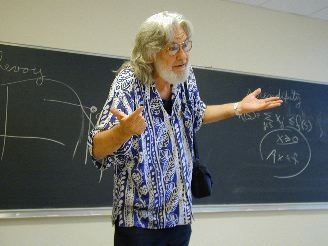
\includegraphics[width=1.0\textwidth]{Edmonds.jpg}%
     \end{minipage}%
     \qquad
      \begin{minipage}{0.30\textwidth}
      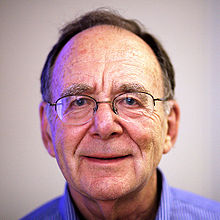
\includegraphics[width=1.0\textwidth]{Karp.jpg}%
     \end{minipage}%
   \end{center}
   \caption{Jack Edmonds, and Richard Karp }
 \end{figure}
\begin{itemize}
 \item
The algorithm was first published by Yefim Dinitz in 1970 and independently published by Jack Edmonds and Richard Karp in 1972.
\end{itemize}
} 

\frame{
\frametitle{{\sc {\sc Edmonds-Karp}} algorithm }

{\sc {\sc Edmonds-Karp}}$(G)$\\
  \begin{algorithmic}[1]
    \STATE Initialize $f(e)=0$ for all $e$.
    \WHILE{there is a $s-t$ path in $G_f$}
    \STATE Find  \textcolor{red}{\bf a shortest $s-t$} path $p$ in  $G_f$ using  \textcolor{red}{\bf $BFS$}; 
    \STATE $f = ${\sc augment}$(p, f)$;
    \ENDWHILE
     \RETURN{$f$};
  \end{algorithmic}
(a demo)
} 

\frame{
%\frametitle{Analysis}

\begin{theorem}{}
{\sc Edmonds-Karp} algorithm runs in $O(m^{2} n)$ time. 
\end{theorem} 
\begin{proof}
\begin{itemize}
	\item During the execution of {\sc Edmonds-Karp} algorithm, an edge $e=(u,v)$ serves as  \textcolor{red}{\bf bottleneck} edge at most $\frac{n}{2}$ times.
	\item Thus, the {\tt while}  loop will be executed at most $\frac{n}{2} m$ times since there are $m$ edges in total.
	\item It takes $O(m)$ time to find the shortest path using BFS and subsequently augment flow along the path. 
\end{itemize}
\end{proof}
\begin{itemize}
	\item {\sc Edmonds-Karp} algorithm is strongly polynomial: its  bound is polynomial in $n$ and $m$, even if capacities are real  numbers, assuming that elementary arithmetic operations on real numbers take unit time.  Strongly polynomial is more natural from combinatorial point of view, as only  arithmetic operation complexity depends on the input size, and other operation counts are independent of the size. 
\end{itemize}

} 

\frame{
\begin{theorem}{}
Any edge $e=(u,v)$ in $G$ acts as \textcolor{red}{bottleneck} at most $\frac{n}{2}$ times. 
\end{theorem}
\begin{proof} 
	\begin{itemize}
	\begin{small}
	\item For a residual graph $G_{f}$, we first  category all nodes into levels $L_{0}, L_{1}, ...$, where $L_{0}=\{s \}$, and $L_{i}$ contains all nodes $v$ such that the shortest path from $s$ to $v$ has $i$ hops. We use $d_f(u)$ to denote the level number of node $u$, i.e. the shortest distance from $s$ to $u$ in $G_f$.  
%	\item Any shortest $s-v$ path contains exactly one node from one level. 
	\item Consider the two consecutive  occurrences of edge $e=(u, v)$  as bottleneck, say at step $k$ and step $k'''$. 	
	\begin{itemize}
		\begin{small}
		\item 
	% a   \textcolor{red}{bottleneck} edge $e=(u,v)$ with node levels: $u\in L_{i}$ and $v \in L_{i+1}$. 
 		 At step $k$, we have $d_f(v) = d_f(u) + 1$. Note that after flow augmentation, the bottleneck edge $e=(u,v)$ will be reversed. 
		\item At step $k'''$,  $e=(u,v)$ becomes a \textcolor{red}{bottleneck} edge again, which  means that $e'=(v,u)$ should be reversed first before step $k'''$, say at step $k''$. 
		\item At step $k''$, we have $d_{f''}(u) = d_{f''}(v) + 1$. 
		\end{small}
	\end{itemize} 
	\item Thus $d_{f''}(u) = d_{f''}(v) + 1 \geq d_{f'}(v) + 1 \geq d_f(u)+2$.  The lemma holds as for any node, its maximal level is at most $n$ and its level number never decrease (why?).   
		\end{small}
\end{itemize} 
\end{proof} 
} 



\frame{
\frametitle{Analyzing the {\sc Edmonds-Karp} algorithm}

\begin{figure}
\begin{tikzpicture}[scale=1, auto,swap]
 
    \def\y{0};
   \def\r{1.2};    
    \node[red, ultra thick] at (-1.5*\r, 0+\y) {Step $k:$};
    
    \foreach \pos/\name in {{(0*\r,0+\y)/s}, {(2*\r,0+\y)/u}, {(3*\r,0+\y)/v}, {(5*\r,0+\y)/t}}
        \node[middlevertex, draw, fill=blue!20] (\name) at \pos {$\name$};

    \foreach \source/ \dest /\weight in {s/u/{}, u/v/{},v/t/{} }
        \path[edge, dashed] (\source) -- node[weight] {$\weight$} (\dest);
 
    \foreach \source/ \dest /\weight in {u/v/{} }
        \path[edge, blue] (\source) -- node[weight] {$\weight$} (\dest);
 
       \node[above] at (u.north) {\footnotesize $d_f(u)$};
       \node[above] at (v.north) {\footnotesize $d_f(v)$};
   
          \node[above, red] at (t.north) {\footnotesize $d_f(v)=d_f(u)+1$};


          
       \def\y{-6};
    
    \node[red, ultra thick] at (-1.5*\r, 0+\y) {Step $k''':$};
    
    \foreach \pos/\name in {{(0*\r,0+\y)/s}, {(2*\r,0+\y)/u}, {(3*\r,0+\y)/v}, {(5*\r,0+\y)/t}}
        \node[middlevertex, draw, fill=blue!20] (\name) at \pos {$\name$};

    \foreach \source/ \dest /\weight in {s/u/{}, u/v/{},v/t/{} }
        \path[edge, dashed] (\source) -- node[weight] {$\weight$} (\dest);

    \foreach \source/ \dest /\weight in {u/v/{} }
        \path[edge, blue] (\source) -- node[weight] {$\weight$} (\dest);

       \node[above] at (u.north) {\footnotesize $d_{f'''}(u)$};
       \node[above] at (v.north) {\footnotesize $d_{f'''}(v)$};
       
  %                      \node[above, red] at (t.north) {\footnotesize $d_{f'''}(u)\geq d_f(u)+2$};
 
 
 \pause 
 
       \def\y{-1.5};
    
    \node[red, ultra thick] at (-1.5*\r, 0+\y) {Step $k+1:$};
    
    \foreach \pos/\name in {{(0*\r,0+\y)/s}, {(2*\r,0+\y)/u}, {(3*\r,0+\y)/v}, {(5*\r,0+\y)/t}}
        \node[middlevertex, draw, fill=blue!20] (\name) at \pos {$\name$};

    \foreach \source/ \dest /\weight in {s/u/{}, v/u/{},v/t/{} }
        \path[edge, dashed] (\source) -- node[weight] {$\weight$} (\dest);

    \foreach \source/ \dest /\weight in {v/u/{} }
        \path[edge, red] (\source) -- node[weight] {$\weight$} (\dest);

       \node[above] at (u.north) {\footnotesize $d_{f'}(u)$};
       \node[above] at (v.north) {\footnotesize $d_{f'}(v)$};
       
         \node[above, red] at (t.north) {\footnotesize $d_{f'}(v)\geq d_f(v)$};

       \node[ultra thick, blue] at (2.5*\r, -2.5) {$\vdots$};
  
  \pause
      \def\y{-3.8};
    
    \node[red, ultra thick] at (-1.5*\r, 0+\y) {Step $k'':$};
    
    \foreach \pos/\name in {{(0*\r,0+\y)/s}, {(2*\r,0+\y)/u}, {(3*\r,0+\y)/v}, {(5*\r,0+\y)/t}}
        \node[middlevertex, draw, fill=blue!20] (\name) at \pos {$\name$};


    \foreach \source/ \dest /\weight in {v/u/{} }
        \path[edge, dashed] (\source) -- node[weight] {$\weight$} (\dest);
    
    \foreach \source/ \dest /\weight in {v/u/{} }
        \path[edge, red] (\source) -- node[weight] {$\weight$} (\dest);
    
       \node[above] at (u.north) {\footnotesize $d_{f''}(u)$};
       \node[above] at (v.north) {\footnotesize $d_{f''}(v)$};
       
       
            \draw[ thick, dashed, ->] (s) to[out=30, in=150] (v);
             \draw[ thick, dashed, below, ->] (u) to [out=-30, in=210] (t);

          \node[ultra thick, blue] at (2.5*\r, -4.5) {$\vdots$};
              \node[above, red] at (t.north) {\footnotesize $d_{f''}(u)=d_{f''}(v)+1$};

  \pause
             \node[above, red] at (5*\r, 0-6+0.25) {\footnotesize $d_{f'''}(u)\geq d_f(u)+2$};
 

   \end{tikzpicture}
\end{figure}


}


\frame{
	\frametitle{Node's level number never decrease}
\begin{theorem}{}
Consider a flow $f$ and the corresponding residual graph $G_{f}$. Suppose a shortest-path $p$ from $s$ to $t$ in  $G_{f}$ was selected for augmentation, forming a new flow $f'$.  Then for any node $v$, $d_f(v) \leq d_{f'}(v)$. 

\end{theorem}
Intuition: For any node $v$, its shortest-path distance $d_{f}(v)$ in residual graph $G_{f}$ never decrease if  shortest augmentation paths were selected for augmentation.  

 \begin{figure}
\begin{tikzpicture}[scale=1, auto,swap]

   
        
        
    \def\dx{0};
    \def\dy{0};	

     \foreach \x/\y/\name in {0/0/s, 2/1/u, 2/-1/v, 4/0/t}
        \node[middlevertex, draw,  fill=blue!20] (\name) at (\x+\dx, \y+\dy) {$\name$};
        
%        \draw[->, thick] (s.15) -- node[below, sloped, midway] {\small $0$} (u.225);
%        \draw[->, thick] (u.195) -- node[above, sloped, midway] {\small $1$} (s.45);
%
%        \draw[->, thick] (u.285) -- node[above, sloped, midway] {\small $0$} (v.75);
%        \draw[->, thick, green] (v.105) -- node[above, sloped, midway, green] {\small $1$} (u.255);
%
%        \draw[->, thick] (v.15) -- node[below, sloped, midway] {\small $0$} (t.225);
%        \draw[->, thick] (t.195) -- node[above, sloped, midway] {\small $1$} (v.45);

        
    \foreach \source/ \dest /\weight in {s/u/{4}}
        \path[edge, sloped, midway, above, allow upside down] (\source) -- node[weight] {\footnotesize $\weight$} (\dest);
        
    \foreach \source/ \dest /\weight in {u/t/{3}}
        \path[edge, sloped, midway, above, allow upside down] (\source) -- node[weight] {\footnotesize $\weight$} (\dest);        
        
    \foreach \source/ \dest /\weight in {u/v/{1}}
        \path[edge, sloped, midway, above, allow upside down] (\source) -- node[weight] {\footnotesize $\weight$} (\dest);
        
    \foreach \source/ \dest /\weight in {v/t/{3}}
        \path[edge, sloped, midway, below, allow upside down, green] (\source) -- node[weight] {\footnotesize $\weight$} (\dest);

    \foreach \source/ \dest /\weight in {s/v/{2}}
        \path[edge, sloped, midway, below, allow upside down, green] (\source) -- node[weight] {\footnotesize $\weight$} (\dest);
       
   \node[ultra thick, red, below] at (0-0.6+\dx, 0.4+\dy) {$G_f$};     

   \node[ultra thick, blue, below] at (0+\dx, 0-0.3+\dy) {\footnotesize $d_{f}(s) = 0$};     
    \node[ultra thick, blue, below] at (2+\dx, 1+0.8+\dy) {\footnotesize $d_{f}(u) = 1$};     
   \node[ultra thick, blue, below] at (v.south) {\footnotesize $d_{f}(v) = 1$};     
   \node[ultra thick, blue, below] at (4+\dx, 0-0.3+\dy) {\footnotesize $d_{f}(t) = 2$};     



        
        
    \def\dx{5.7};
    \def\dy{0};	

     \foreach \x/\y/\name in {0/0/s, 2/1/u, 2/-1/v, 4/0/t}
        \node[middlevertex, draw,  fill=blue!20] (\name) at (\x+\dx, \y+\dy) {$\name$};
        
%        \draw[->, thick] (s.15) -- node[below, sloped, midway] {\small $0$} (u.225);
%        \draw[->, thick] (u.195) -- node[above, sloped, midway] {\small $1$} (s.45);
%
%        \draw[->, thick] (u.285) -- node[above, sloped, midway] {\small $0$} (v.75);
%        \draw[->, thick, green] (v.105) -- node[above, sloped, midway, green] {\small $1$} (u.255);
%
%        \draw[->, thick] (v.15) -- node[below, sloped, midway] {\small $0$} (t.225);
%        \draw[->, thick] (t.195) -- node[above, sloped, midway] {\small $1$} (v.45);

        \draw[->, thick] (v.15) -- node[below, sloped, midway] {\small $1$} (t.225);
        \draw[->, thick] (t.195) -- node[above, sloped, midway] {\small $2$} (v.45);

        
    \foreach \source/ \dest /\weight in {s/u/{4}}
        \path[edge, sloped, midway, above ] (\source) -- node[weight] {\footnotesize $\weight$} (\dest);
        
    \foreach \source/ \dest /\weight in {u/t/{3}}
        \path[edge, sloped, midway, above] (\source) -- node[weight] {\footnotesize $\weight$} (\dest);        
        
    \foreach \source/ \dest /\weight in {u/v/{1}}
        \path[edge, sloped, midway, above, allow upside down] (\source) -- node[weight] {\footnotesize $\weight$} (\dest);
        
%    \foreach \source/ \dest /\weight in {t/v/{2}}
%        \path[edge, sloped, midway, below] (\source) -- node[weight] {\footnotesize $\weight$} (\dest);

    \foreach \source/ \dest /\weight in {v/s/{2}}
        \path[edge, sloped, midway, below] (\source) -- node[weight] {\footnotesize $\weight$} (\dest);
       
   \node[ultra thick, red, below] at (0-0.6+\dx, 0.4+\dy) {$G_{f'}$};     

   \node[ultra thick, blue, below] at (0+\dx, 0-0.3+\dy) {\footnotesize $d_{f'}(s) = 0$};     
    \node[ultra thick, blue, below] at (2+\dx, 1+0.8+\dy) {\footnotesize $d_{f'}(u) = 1$};     
   \node[ultra thick, blue, below] at (v.south) {\footnotesize $d_{f'}(v) = 2$};     
   \node[ultra thick, blue, below] at (4+\dx, 0-0.3+\dy) {\footnotesize $d_{f'}(t) = 2$};     
              
   \end{tikzpicture}
\end{figure}

} 

\frame{
\begin{Proof}
	\begin{itemize}
		\item First we claim that for any edge $(v_{i}, v_{j})$ in $G_{f'}$, $d_f(v_{j}) \leq d_f(v_{i}) + 1$.
			\begin{itemize}
				\item Case 1:  $(v_{i}, v_{j})$ in $G_{f}$, e.g. $(u, v)$: Obvious.   
				\item Case 2: $(v_{i}, v_{j})$ not in $G_{f}$: Take $(u, s)$ as an example. 
				$(s, u)$ should be in the augmentation (shortest) path in $G_{f}$ and thus  $d_f(u) = d_f(s) + 1$. 
			\end{itemize}
		\item Next, suppose $d_{f'}(v) = r$. Let $(s, v_1, ..., v_{r-1}, v)$ 
be a shortest path to $v$ in $G_{f'}$. We have: 
 \begin{eqnarray}
 d_f(v) &\leq &  d_f(v_{r-1}) + 1 \nonumber\\ 
    	  &\leq &  d_f(v_{r-2}) + 2 \nonumber\\
    	  &..... &  \nonumber\\
	&\leq &  d_f(s) + r \nonumber\\
	& = & r \nonumber
 \end{eqnarray}
\end{itemize} 
\end{Proof}
}


%\frame{
%	\frametitle{Proof}
%	\begin{itemize}
%		\item Consider a flow $f$ and the corresponding residual graph $G_{f}$. Suppose the shortest-path $p$ from $s$ to $t$ in  $G_{f}$ was selected for augmentation, forming a new flow $f'$. 
%		\item Assume for contradiction that there is a node $v$ such that 
%			$d_{f'}(v) < d_{f}(v)$.  
%		 Without loss of generality, let $v$ be such a  node with the minimum $d_{f'}(v)$ in $G_{f'}$, and let  $p'=s\leadsto u\rightarrow v$ denote the shortest-path to $v$ in $G_{f'}$. Thus we have: 
%			\begin{itemize}
%				\item  $d_{f'}(v) = d_{f'}(u)+1$, and
%				\item  $d_{f'}(u) \geq d_{f}(u)$ due to the selection of $v$.  
%			\end{itemize}
%		\item Next we claim that a contradiction occurs regardless of the edge $u\rightarrow v \in G_{f}$ and thus prove the lemma. $\qed$ 
%%		 $Let's investigate whether $u\rightarrow v$ appears in $G_f$. There are two cases: 
%%			\begin{itemize}
%%				\item $u\rightarrow v \in G_{f}$. 
%%				\item $u\rightarrow v \notin G_{f}$ but $\in G_{f'}$
%%			\end{itemize}				
%%		 and in both cases, a contradiction occurs. Hence the lemma follows. 
%	\end{itemize}
%}
%
%\frame{
%	\frametitle{Case 1: a contradiction occurs if $u\rightarrow v \in G_{f}$}
%
%\begin{figure}
%\begin{tikzpicture}[scale=1, auto,swap]
% 
%    \def\y{0};
%    
%    \node[red, ultra thick] at (-0.8, 0+\y) {$G_{f'}$: };
%    
%    \foreach \pos/\name in {{(0*\r,0+\y)/s}, {(2*\r,0+\y)/u}, {(3*\r,0+\y)/v}}
%        \node[middlevertex, draw, fill=blue!20] (\name) at \pos {$\name$};
%
%    \foreach \source/ \dest /\weight in {s/u/{}, u/v/{}}
%        \path[edge, dashed] (\source) -- node[weight] {$\weight$} (\dest);
% 
%    \foreach \source/ \dest /\weight in {u/v/{} }
%        \path[edge, blue] (\source) -- node[weight] {$\weight$} (\dest);
% 
%       \node[above] at (u.north) {\footnotesize $d_{f'}(u)$};
%       \node[above] at (v.north) {\footnotesize $d_{f'}(v)$};
%   
%          \node[above, blue] at ( 5, 0+\y+0.25) {\footnotesize $d_{f'}(v)=d_{f'}(u)+1$};
%
%     \def\y{+1.5};
%    
%    \node[red, ultra thick] at (-0.8, 0+\y) {$G_{f}$: };
%    
%    \foreach \pos/\name in {  {(2*\r,0+\y)/u}, {(3*\r,0+\y)/v}}
%        \node[middlevertex, draw, fill=blue!20] (\name) at \pos {$\name$};
%
% 
%    \foreach \source/ \dest /\weight in {u/v/{} }
%        \path[edge, blue] (\source) -- node[weight] {$\weight$} (\dest);
% 
%       \node[above] at (u.north) {\footnotesize $d_{f}(u)$};
%       \node[above] at (v.north) {\footnotesize $d_{f}(v)$};
%   
%          \node[above, blue] at (5, 0+\y+0.25) {\footnotesize $d_{f}(v)\leq d_{f}(u)+1$};
%
%    \node[ultra thick] at (1, 0+\y) {$\dots$};
%    \node[ultra thick] at (4, 0+\y) {$\dots$};
%
%              
%   \end{tikzpicture}
%\end{figure}
%
%			\begin{itemize}
%				\item We have $d_f(u) + 1 \geq d_f(v)$. 
%				\item Thus $d_{f'}(v) = d_{f'}(u) + 1 \geq d_f(u) + 1 \geq d_f(v)$, which contradicts the assumption that $d_{f'}(v) < d_{f}(v)$. 
%			\end{itemize}	
%}
%
%\frame{
%	\frametitle{Case 2: a contradiction occurs if $u\rightarrow v \notin G_{f}$ but $\in G_{f'}$ }
%
%\begin{figure}
%\begin{tikzpicture}[scale=1, auto,swap]
% 
%    \def\y{0};
%    
%    \node[red, ultra thick] at (-0.8, 0+\y) {$G_{f'}$: };
%    
%    \foreach \pos/\name in {{(0*\r,0+\y)/s}, {(2*\r,0+\y)/u}, {(3*\r,0+\y)/v}}
%        \node[middlevertex, draw, fill=blue!20] (\name) at \pos {$\name$};
%
%    \foreach \source/ \dest /\weight in {s/u/{}, u/v/{}}
%        \path[edge, dashed] (\source) -- node[weight] {$\weight$} (\dest);
% 
%    \foreach \source/ \dest /\weight in {u/v/{}}
%        \path[edge, blue] (\source) -- node[weight] {$\weight$} (\dest);
% 
%       \node[above] at (u.north) {\footnotesize $d_{f'}(u)$};
%       \node[above] at (v.north) {\footnotesize $d_{f'}(v)$};
%   
%       \node[above, blue] at (5, 0+\y+0.25) {\footnotesize $d_{f'}(v)=d_{f'}(u)+1$};
%
%
%%    \def\y{0};
%%    
%%    \node[red, ultra thick] at (-0.8, 0+\y) {$G_{f'}$: };
%%    
%%    \foreach \pos/\name in {{(0*\r,0+\y)/s}, {(2*\r,0+\y)/u}, {(3*\r,0+\y)/v}, {(5*\r,0+\y)/t}}
%%        \node[middlevertex, draw, fill=blue!20] (\name) at \pos {$\name$};
%%
%%    \foreach \source/ \dest /\weight in {s/u/{}, u/v/{},v/t/{} }
%%        \path[edge, dashed] (\source) -- node[weight] {$\weight$} (\dest);
%% 
%%    \foreach \source/ \dest /\weight in {u/v/{} }
%%        \path[edge, blue] (\source) -- node[weight] {$\weight$} (\dest);
%% 
%%       \node[above] at (u.north) {\footnotesize $d_{f'}(u)$};
%%       \node[above] at (v.north) {\footnotesize $d_{f'}(v)$};
%%   
%%          \node[above, blue] at (t.north) {\footnotesize $d_{f'}(v)=d_{f'}(u)+1$};
%
%
%    \def\y{+2};
%    \node[red, ultra thick] at (-0.8, 0+\y) {$G_{f}:$};
%    
%    \foreach \pos/\name in {{(0*\r,0+\y)/s}, {(2*\r,0+\y)/u}, {(3*\r,0+\y)/v}, {(5*\r,0+\y)/t}}
%        \node[middlevertex, draw, fill=blue!20] (\name) at \pos {$\name$};
%
%    \foreach \source/ \dest /\weight in {v/u/{} }
%        \path[edge, dashed] (\source) -- node[weight] {$\weight$} (\dest);
%    
%    \foreach \source/ \dest /\weight in {v/u/{} }
%        \path[edge, red] (\source) -- node[weight] {$\weight$} (\dest);
%    
%       \node[above] at (u.north) {\footnotesize $d_{f}(u)$};
%       \node[above] at (v.north) {\footnotesize $d_{f}(v)$};
%       
%       
%            \draw[ thick, dashed, ->] (s) to[out=30, in=150] (v);
%             \draw[ thick, dashed, below, ->] (u) to [out=-30, in=210] (t);
%
%%          \node[ultra thick, blue] at (2.5, -4.5) {$\vdots$};
%              \node[above, blue] at (t.north) {\footnotesize $d_{f}(u)=d_{f}(v)+1$};
%
%              
%   \end{tikzpicture}
%\end{figure}
%
%			\begin{itemize}
%				\item The fact $u\rightarrow v \notin G_{f}$ but $\in G_{f'}$ implies that $u\rightarrow v$ appears through reversing  $v\rightarrow u$, which should exists in the augmentation path in $G_{f}$ chosen by {\sc {\sc Edmonds-Karp}} algorithm. Thus, we have $d_f(u) = d_f(v) + 1$. 
%				\item We further have $d_{f'}(v) = d_{f'}(u) + 1 \geq d_f(u) + 1 =d_f(v) + 2$,  contradicting the assumption that $d_{f'}(v) < d_{f}(v)$. 
%			\end{itemize}
%
%
%}
%

%\frame{
%	\frametitle{In both cases, a contradiction occurs} 
%	\begin{itemize}
%		\item $u\rightarrow v \in G_{f}$: 
%			\begin{itemize}
%				\item We have $d_f(u) + 1 \geq d_f(v)$. 
%				\item Thus $d_{f'}(v) = d_{f'}(u) + 1 \geq d_f(u) + 1 \geq d_f(v)$. A contradiction with the assumption. 
%			\end{itemize}	
%		\item $u\rightarrow v \notin G_{f}$ but $\in G_{f'}$:
%			\begin{itemize}
%				\item This can happen only if $v\rightarrow u$ exists in $p$, one of the shortest paths from $s$ to $t$ in $G_f$.  
%				\item Thus, we have $d_f(u) = d_f(v) + 1$. 
%				\item Thus another contradiction occurs: 
%					$d_{f'}(v) = d_{f'}(u) + 1 \geq d_f(u) + 1 =d_f(v) + 2$. 
%			\end{itemize}
%	\end{itemize}
%}

\frame{
\begin{block}{}
 Improvement 3: Dinitz' algorithm and its variant Dinic's algorithm  
\end{block}
}


\frame{
	 \begin{figure}%
   \begin{center}%
      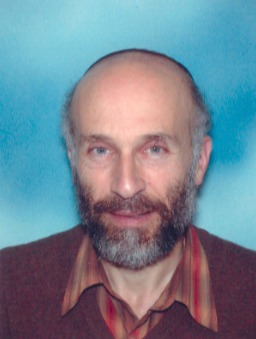
\includegraphics[width=2in]{Y.Dinitz.jpg}%
   \end{center}
   \caption{Yefim Dinitz} 
   \end{figure}

} 

%\frame{
%\frametitle{Dinic's algorithm }
%\begin{itemize}
%\item Motivation: The initial intention was just to accelerate FF by means of a smart data structure 
%\item Recall that all part of FF cost $|p|$ time;
%\item Thus, finding a shortest path is important; 
%\item However, it takes $O(m)$ time to find a path by using BFS. 
%\item This is the bottleneck. 
%\end{itemize}
%
%} 

\frame{
	\frametitle{A brief history}
	
	\begin{itemize}
		\item Y. Dinitz worked in a group led by G. Adel'son Vel'sky, who (together with E. Landis) designed the famous AVL-tree data structure. Y. Dinitz absorbed the essential issues, including: 
		\begin{itemize}
			\item Design efficient algorithms based on deep investigation on problem structures; 
			\item The technique of \textcolor{red}{\bf data structure maintenance}; 
			\item Amortized analysis technique (about 17 years before the paper by R. Tarjan). 
		\end{itemize}

	\end{itemize}

}

\frame{
\frametitle{The original Dinitz' algorithm } 
\begin{itemize}
\item Basic idea: 
\begin{itemize}
\item The initial intention was just to accelerate {\sc {\sc Ford-Fulkerson}} algorithm by means of a smart data structure. 
\item Note that finding an augmentation path takes $O(m)$ time and becomes a  bottleneck of {\sc {\sc Ford-Fulkerson}} algorithm. If only BFS tree was used, saturation of a bottleneck edge will disconnect $s$ and $t$. Thus, it is invaluable to save \textcolor{red}{\bf all information} gathered in  BFS for subsequent iterations.  
\item For this aim, the \textcolor{red}{\bf BFS tree} is enriched to \textcolor{red}{\bf layered network}: 
\begin{itemize}
\item BFS tree:  recording  \textcolor{red}{\bf  only the first edge found to a node $v$;} 
\item Layered network: recording \textcolor{red}{\bf all the edges residing on shortest $s-t$ paths in residual graph}. Once layer numbers were calculated for nodes, a shortest $s-t$ path could be found in $O(n)$ time rather than $O(m)$ time.   %Note that layered network has an advantage to  record \textcolor{red}{all} shortest $s-t$ paths. 
\end{itemize}
\end{itemize}
\end{itemize}


\begin{figure}
\begin{tikzpicture}[scale=1, auto,swap]
 
    \def\x{0};
    \def\y{0.7};
    \foreach \pos/\name in {{(0+\x, 0)/s}, {(1+\x,\y)/u}, {(1+\x, -\y)/v}, {(2+\x, \y)/w}, {(2+\x, -\y)/r}, {(3+\x, \y)/tt}, {(3+\x, 0)/t}}
        \node[smallvertex, draw, fill=blue!20] (\name) at \pos {};
 
    \foreach \source/ \dest in {s/u, s/v, v/u, u/w, u/r, v/r, r/w, w/tt, w/t, tt/t, r/t}
        \path[edge] (\source) -- node  {} (\dest);
 
       \node[below] at (s.south) {\small $s$};
       \node[below] at (t.south) {\small $t$};       
      \node[below, ultra thick, blue] at (\x+1.5, -\y-0.3) {Residual graph $G_{f}$}; 


    \def\x{4};
    \def\y{0.7};
    \foreach \pos/\name in {{(0+\x, 0)/s}}
        \node[smallvertex, draw, fill=blue!20] (\name) at \pos {};
 
     \foreach \pos/\name in {{(1+\x,\y)/u}, {(1+\x, -\y)/v}}
        \node[smallvertex, draw, fill=red!20] (\name) at \pos {};
        
            \foreach \pos/\name in {{(2+\x, \y)/w}, {(2+\x, -\y)/r}}
        \node[smallvertex, draw, fill=green] (\name) at \pos {};
        
            \foreach \pos/\name in {{(3+\x, \y)/tt}, {(3+\x, 0)/t}}
        \node[smallvertex, draw, fill=yellow] (\name) at \pos {};
        
     \foreach \source/ \dest in {s/u, s/v,   u/w, u/r,   w/tt, w/t}
        \path[edge] (\source) -- node  {} (\dest);
 
       \node[below] at (s.south) {\small $s$};
       \node[below] at (t.south) {\small $t$};       
      \node[below, ultra thick, blue] at (\x+1.5, -\y-0.3) {BFS tree}; 


    \def\x{8};
    \def\y{0.7};
    \foreach \pos/\name in {{(0+\x, 0)/s}}
        \node[smallvertex, draw, fill=blue!20] (\name) at \pos {};
 
     \foreach \pos/\name in {{(1+\x,\y)/u}, {(1+\x, -\y)/v}}
        \node[smallvertex, draw, fill=red!20] (\name) at \pos {};
        
            \foreach \pos/\name in {{(2+\x, \y)/w}, {(2+\x, -\y)/r}}
        \node[smallvertex, draw, fill=green] (\name) at \pos {};

         \foreach \pos/\name in {{(3+\x, \y)/tt}}
        \node[smallvertex, draw, dashed, fill=yellow!10] (\name) at \pos {};

            \foreach \pos/\name in {{(3+\x, 0)/t}}
        \node[smallvertex, draw, fill=yellow] (\name) at \pos {};
 
    \foreach \source/ \dest in {s/u, s/v,  u/w, u/r, v/r,  w/t, r/t}
        \path[edge] (\source) -- node  {} (\dest);
 
     \foreach \source/ \dest in {w/tt}
        \path[edge, dashed] (\source) -- node  {} (\dest);

       \node[below] at (s.south) {\small $s$};
       \node[below] at (t.south) {\small $t$};       
      \node[below, ultra thick, blue] at (\x+1.5, -\y-0.3) {Layered network $N_f$}; 





   \end{tikzpicture}
\end{figure}

%\begin{figure}
% 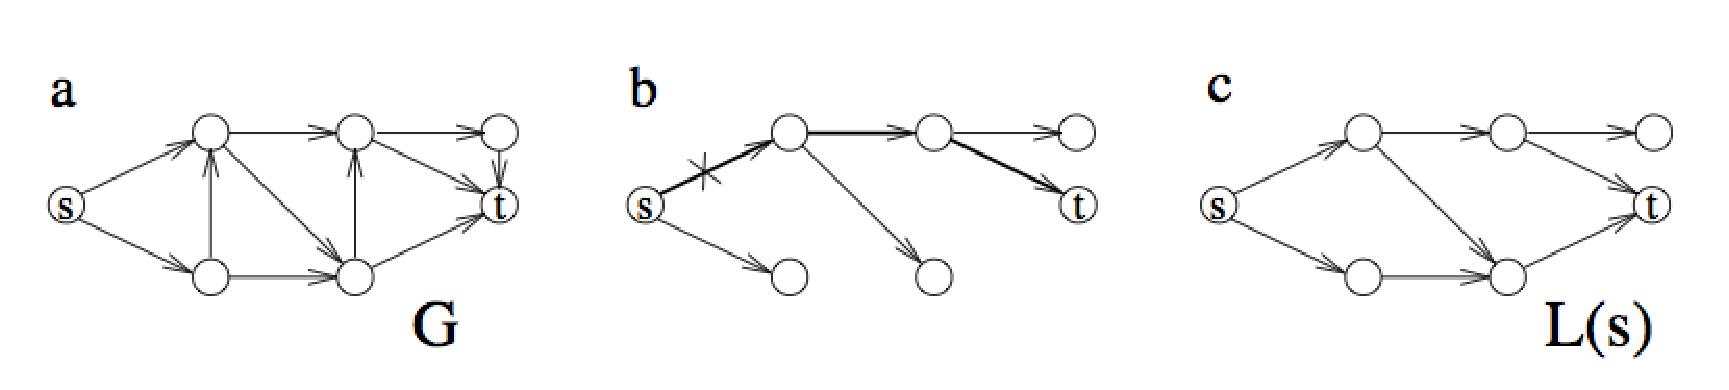
\includegraphics[width=4in] {L10-dinic1.eps}
%\end{figure}
} 

%\frame{
%\frametitle{{\sc Dinitz} algorithm }
%
%{\sc Dinitz} algorithm:\\
%  \begin{algorithmic}[1]
%    \STATE{Initialize $f(e)=0$ for all $e$.}
%    \WHILE{\texttt{TRUE} }
%    \STATE{Construct layered network $N_f$ from residual graph $G_f$ using extended BFS;}
%    \IF{$N_f$ is empty }
%    \RETURN {$f$};
%    \ENDIF
%    \STATE{$L=$ the union of all shortest augmentation paths};
%    \STATE{$p$ = a shortest path;  } 
%    \STATE{{\sc augment}$(f, p)$;}
%    \ENDIF
%    \STATE{find a blocking flow $f'$ in $N_f$; }
%    \STATE{augment flow $f$ by $f'$; }
%    \ENDWHILE
%  \end{algorithmic}
%(See ppt for a demo)
%} 

\frame{
\frametitle{Dinic's algorithm: layered network + blocking flow } 
\begin{itemize}
	\item Shimon Even and Alon Itai understood the paper by Y. Dinitz except for the \textcolor{black}{layered network maintenance}  and that by A. Karzanov. The gaps were spanned by using:	
		\begin{enumerate}
			\item \textcolor{red}{\bf Blocking flow} (first proposed by A. Karzanov and implicit in the paper by Y. Dinitz): A blocking flow, also known as \textcolor{red}{\bf shortest saturation flow}
			aims to saturate all shortest $s-t$ paths in a residual network. After augmenting with a blocking flow, 
			the level number of node $t$ increases by \textcolor{red}{\bf at least 1}.
			\item \textcolor{red}{\bf DFS}: Dinic's algorithm uses DFS technique to find a shortest path  in  layered network. Only $O(n)$ time is needed as it exploits level numbers of nodes. In contrast, Edmonds-Karp algorithm  uses BFS technique to find a shortest path in residual graph, which needs  $O(m)$ time.
			 
		\end{enumerate}
	%\item Note: the layered network was relaxed to include only all the augmentation paths of length $l$; 
	\item Note: when running on bi-partite graph, the Dinic's algorithm turns into the Hopcroft-Karp algorithm. 
\end{itemize}
}


\frame{
\frametitle{{\sc Dinic's} algorithm }
{\sc Dinic's-Max-Flow}$(G)$
  \begin{algorithmic}[1]
    \STATE{Initialize $f(e)=0$ for all $e$.}
    \WHILE{\texttt{TRUE} }
    \STATE{Construct \textcolor{red}{\bf layered network} $N_f$ from \textcolor{red}{\bf residual graph} $G_f$} using extended BFS technique; 
    \IF{$t$ is unreachable from $s$ in $G_f$}
    \STATE{break; } 
    \ENDIF
    \STATE{Find a \textcolor{red}{\bf blocking flow} $b_{f}$ in $N_f$ using \textcolor{red}{\bf DFS} technique guided by the layered network; }
    \STATE{Augment flow $f = f + b_{f}$;}
    \ENDWHILE
    \RETURN{$f$};
  \end{algorithmic}
 }

\frame{
\frametitle{Constructing layered network from residual network}
{\sc Construct-Layered-Network}$(G_f)$
  \begin{algorithmic}[1]
    \STATE{Set $d_{f}(s) = 0$, $d_{f}(v) = \infty$ for node $v\neq s$, and  add $s$ into queue $Q$;}
    \STATE{Set layered network $N_{f} = (V_{f}, E_{f})$ as $V_{f}=\{s\}$ and $E_{f}=\{\}$;}
    \WHILE{$Q$ is not empty}
    	\STATE{$v = Q.dequeue()$;}
	\FOR{each edge $(v, w)$ in $G_{f}$}
		\IF{$d_{f}(w) = \infty$}
			\STATE{$Q.enqueue(w);$ $d_{f}(w) = d_{f}(v) + 1;$}
			\STATE{$V_{f} = V_{f} \cup \{w\};$  $E_{f} = E_{f} \cup \{(v, w)\};$}  
		\ENDIF
		\IF{$d_{f}(w) = d_{f}(v) + 1$}
			\STATE{$E_{f} = E_{f} \cup \{(v, w)\};$}
		\ENDIF
	\ENDFOR
    \ENDWHILE	
    \STATE{Perform BFS in $N_{f}$ from $t$ with all edges directions reversed, and delete $v$ from $N_{f}$ if $v$ cannot be visited;} 
    \RETURN{$N_{f}$};
  \end{algorithmic}
}
 
\frame{
	\frametitle{Constructing layered network from residual network: an example} 
	
	\begin{figure}
\begin{tikzpicture}[scale=1, auto,swap]
 
    \def\x{0};
    \def\y{0.7};
    \foreach \pos/\name in {{(0+\x, 0)/s}, {(1+\x,\y)/u}, {(1+\x, -\y)/v}, {(2+\x, \y)/w}, {(2+\x, -\y)/r}, {(3+\x, \y)/tt}, {(3+\x, 0)/t}}
        \node[smallvertex, draw, fill=blue!20] (\name) at \pos {};
 
    \foreach \source/ \dest in {s/u, s/v, v/u, u/w, u/r, v/r, r/w, w/tt, w/t, tt/t, r/t}
        \path[edge] (\source) -- node  {} (\dest);
 
       \node[below] at (s.south) {\small $s$};
       \node[below] at (t.south) {\small $t$};       
      \node[below, ultra thick, blue] at (\x+1.5, -\y-0.3) {Residual graph $G_{f}$}; 


    \def\x{4};
    \def\y{0.7};
    \foreach \pos/\name in {{(0+\x, 0)/s}}
        \node[smallvertex, draw, fill=blue!20] (\name) at \pos {};
 
     \foreach \pos/\name in {{(1+\x,\y)/u}, {(1+\x, -\y)/v}}
        \node[smallvertex, draw, fill=red!20] (\name) at \pos {};
        
            \foreach \pos/\name in {{(2+\x, \y)/w}, {(2+\x, -\y)/r}}
        \node[smallvertex, draw, fill=green] (\name) at \pos {};
        
            \foreach \pos/\name in {{(3+\x, \y)/tt}, {(3+\x, 0)/t}}
        \node[smallvertex, draw, fill=yellow] (\name) at \pos {};
        
     \foreach \source/ \dest in {s/u, s/v,   u/w, u/r,   w/tt, w/t}
        \path[edge] (\source) -- node  {} (\dest);
 
       \node[below] at (s.south) {\small $s$};
       \node[below] at (t.south) {\small $t$};       
      \node[below, ultra thick, blue] at (\x+1.5, -\y-0.3) {BFS tree}; 


    \def\x{8};
    \def\y{0.7};
    \foreach \pos/\name in {{(0+\x, 0)/s}}
        \node[smallvertex, draw, fill=blue!20] (\name) at \pos {};
 
     \foreach \pos/\name in {{(1+\x,\y)/u}, {(1+\x, -\y)/v}}
        \node[smallvertex, draw, fill=red!20] (\name) at \pos {};
        
            \foreach \pos/\name in {{(2+\x, \y)/w}, {(2+\x, -\y)/r}}
        \node[smallvertex, draw, fill=green] (\name) at \pos {};

         \foreach \pos/\name in {{(3+\x, \y)/tt}}
        \node[smallvertex, draw, dashed, fill=yellow!10] (\name) at \pos {};

            \foreach \pos/\name in {{(3+\x, 0)/t}}
        \node[smallvertex, draw, fill=yellow] (\name) at \pos {};
 
    \foreach \source/ \dest in {s/u, s/v,  u/w, u/r, v/r,  w/t, r/t}
        \path[edge] (\source) -- node  {} (\dest);
 
     \foreach \source/ \dest in {w/tt}
        \path[edge, dashed] (\source) -- node  {} (\dest);

       \node[below] at (s.south) {\small $s$};
       \node[below] at (t.south) {\small $t$};       
      \node[below, ultra thick, blue] at (\x+1.5, -\y-0.3) {Layered network $N_f$}; 





   \end{tikzpicture}
\end{figure}

\begin{itemize}
	\item The difference from the standard BFS procedure is that for any edge $(v, w)$ with $d_{f}(w) = d_{f}(v) + 1$ will be added to $N_{f}$ even if $w$ has already been added to $Q$. Thus, for each vertex $v$, exactly all edges in shortest paths from $s$ to $v$ are added in $N_{f}$. 
	\item The nodes (and their incident edges) not on the shortest paths from $s$ to $t$ will be  removed from $N_{f}$, e.g., the node in dash. 
\end{itemize}
}

\frame{
	\frametitle{Finding blocking flow in layered network $N_{f}$ }

{\sc Dinic-Blocking-Flow}$(N_f)$
  \begin{algorithmic}[1]
  	\STATE{Set $b_{f}$ as $0$-flow;}
    	\WHILE{there exists an edge from $s$ in $N_{f}$}
    		\STATE{Find a path $p$ from $s$ of maximal length in $N_{f}$;}
		\IF{$p$ leads to $t$}
			\STATE{$b_{f}=${\sc augment}$(p, b_{f});$ }
			\STATE{Remove from $N_{f}$ the bottleneck edges in $p$; }  
		\ELSE
			\STATE{Delete the last node in $p$ (and incident edges);}
		\ENDIF
    	\ENDWHILE	
    \RETURN{$b_{f}$};
  \end{algorithmic}


}
 
 \frame{ 
 \frametitle{{\sc Dinic's} algorithm }
  \begin{itemize}
  \item The execution of the algorithm can be divided into \textcolor{red}{\bf phases}, each phase consisting of construction of layered network, and finding blocking flow in it. 
  \item 
  Here, a \textcolor{red}{\bf blocking flow} contains  
  \textcolor{red}{\bf a collection of} shortest $s-t$ paths in $G_f$. After saturating these paths, $t$ is unreachable from $s$.  
  \item Intuition: after acquiring a layered network using $O(m)$ time, a blocking flow is found for further augmentation. Each path in blocking flow in only  \textcolor{red}{\bf   $O(n)$}  time guided by the layered network.  In contrast, the  {\sc {\sc Edmonds-Karp}} algorithm augments \textcolor{red}{\bf only one} $s-t$ path after  BFS process using \textcolor{red}{\bf   $O(m)$} time. 
  \end{itemize}
(a demo here)
} 




\frame{
\frametitle{Analysis}

\begin{itemize}
\item Total time: $O(mn^2)$
\begin{itemize}
\item $\#{\tt WHILE} = O(n)$.  (Reason:  After augmentation using block flow,  $d_f(t)$ should increase by at least 1. See next page for proof. )
\item At each iteration, it takes $O(m)$ time to construct layered network using extended BFS, and takes $O(mn)$ time to find a blocking flow since:  
	\begin{enumerate}
		\item  It takes $O(n)$ time to find a shortest $s-t$ path in a layered network $N_{f}$ using DFS technique. 
		\item At least one bottleneck edge in the augmentation path will be saturated and thereafter be removed from $N_{f}$. 
		\item Thus it needs at most $m$ iterations to find a blocking flow. 
	\end{enumerate} 
\end{itemize}

\end{itemize}
} 

\frame{
	\frametitle{$d_{f}(t)$ increases by at least 1 in each phase} 
\begin{theorem}{}
Consider a flow $f$ and the corresponding layered network $N_{f}$. Suppose a blocking flow $b_{f}$ was found in $N_{f}$ and thereafter used for augmentation, forming a new flow $f'$.  Then $d_{f'}(t) \geq d_{f}(t) + 1$. 
\end{theorem}
\begin{itemize}
	\item Note: If only one shortest path, say $s\rightarrow v \rightarrow t$ in the following example,  was selected for augmentation, $d_{f'}(t) = d_f(t) = 2$. In contrast, when all shortest paths were selected for augmentation, $d_{f'}(t) \geq d_f(t) + 1$. 
\end{itemize}
} 

\frame{
	\frametitle{An example}

\begin{figure}
\begin{tikzpicture}[scale=1, auto,swap]
            
    \def\dx{0};
    \def\dy{0};	

     \foreach \x/\y/\name in {0/0/s, 2/1/u, 2/-1/v, 4/0/t}
        \node[middlevertex, draw,  fill=blue!20] (\name) at (\x+\dx, \y+\dy) {$\name$};
        
%        \draw[->, thick] (s.15) -- node[below, sloped, midway] {\small $0$} (u.225);
%        \draw[->, thick] (u.195) -- node[above, sloped, midway] {\small $1$} (s.45);
%
%        \draw[->, thick] (u.285) -- node[above, sloped, midway] {\small $0$} (v.75);
%        \draw[->, thick, green] (v.105) -- node[above, sloped, midway, green] {\small $1$} (u.255);
%
%        \draw[->, thick] (v.15) -- node[below, sloped, midway] {\small $0$} (t.225);
%        \draw[->, thick] (t.195) -- node[above, sloped, midway] {\small $1$} (v.45);

        
    \foreach \source/ \dest /\weight in {s/u/{4}}
        \path[edge, sloped, midway, above, allow upside down] (\source) -- node[weight] {\footnotesize $\weight$} (\dest);
        
    \foreach \source/ \dest /\weight in {u/t/{3}}
        \path[edge, sloped, midway, above, allow upside down] (\source) -- node[weight] {\footnotesize $\weight$} (\dest);        
        
    \foreach \source/ \dest /\weight in {u/v/{1}}
        \path[edge, sloped, midway, above, allow upside down] (\source) -- node[weight] {\footnotesize $\weight$} (\dest);
        
    \foreach \source/ \dest /\weight in {v/t/{3}}
        \path[edge, sloped, midway, below,  allow upside down] (\source) -- node[weight] {\footnotesize $\weight$} (\dest);

    \foreach \source/ \dest /\weight in {s/v/{2}}
        \path[edge, sloped, midway, below,  allow upside down] (\source) -- node[weight] {\footnotesize $\weight$} (\dest);
       
   \node[ultra thick, red, below] at (0-0.6+\dx, 0.4+\dy) {$G_f$};     

   \node[ultra thick, blue, below] at (0+\dx, 0-0.3+\dy) {\footnotesize $d_{f}(s) = 0$};     
    \node[ultra thick, blue, below] at (2+\dx, 1+0.8+\dy) {\footnotesize $d_{f}(u) = 1$};     
   \node[ultra thick, blue, below] at (v.south) {\footnotesize $d_{f}(v) = 1$};     
   \node[ultra thick, blue, below] at (4+\dx, 0-0.3+\dy) {\footnotesize $d_{f}(t) = 2$};     


    \def\dx{6};
    \def\dy{0};	

     \foreach \x/\y/\name in {0/0/s, 2/1/u, 2/-1/v, 4/0/t}
        \node[middlevertex, draw,  fill=blue!20] (\name) at (\x+\dx, \y+\dy) {$\name$};
        
%        \draw[->, thick] (s.15) -- node[below, sloped, midway] {\small $0$} (u.225);
%        \draw[->, thick] (u.195) -- node[above, sloped, midway] {\small $1$} (s.45);
%
%        \draw[->, thick] (u.285) -- node[above, sloped, midway] {\small $0$} (v.75);
%        \draw[->, thick, green] (v.105) -- node[above, sloped, midway, green] {\small $1$} (u.255);
%
%        \draw[->, thick] (v.15) -- node[below, sloped, midway] {\small $0$} (t.225);
%        \draw[->, thick] (t.195) -- node[above, sloped, midway] {\small $1$} (v.45);

        
    \foreach \source/ \dest /\weight in {s/u/{4}}
        \path[edge, sloped, midway, above, allow upside down, green] (\source) -- node[weight] {\footnotesize $\weight$} (\dest);
        
    \foreach \source/ \dest /\weight in {u/t/{3}}
        \path[edge, sloped, midway, above, allow upside down, green] (\source) -- node[weight] {\footnotesize $\weight$} (\dest);        
        
%    \foreach \source/ \dest /\weight in {u/v/{1}}
%        \path[edge, sloped, midway, above, allow upside down] (\source) -- node[weight] {\footnotesize $\weight$} (\dest);
        
    \foreach \source/ \dest /\weight in {v/t/{3}}
        \path[edge, sloped, midway, below, green, allow upside down] (\source) -- node[weight] {\footnotesize $\weight$} (\dest);

    \foreach \source/ \dest /\weight in {s/v/{2}}
        \path[edge, sloped, midway, below, green, allow upside down] (\source) -- node[weight] {\footnotesize $\weight$} (\dest);
       
   \node[ultra thick, red, below] at (0-0.6+\dx, 0.4+\dy) {$N_f$};     

   \node[ultra thick, blue, below] at (0+\dx, 0-0.3+\dy) {\footnotesize $d_{f}(s) = 0$};     
    \node[ultra thick, blue, below] at (2+\dx, 1+0.8+\dy) {\footnotesize $d_{f}(u) = 1$};     
   \node[ultra thick, blue, below] at (v.south) {\footnotesize $d_{f}(v) = 1$};     
   \node[ultra thick, blue, below] at (4+\dx, 0-0.3+\dy) {\footnotesize $d_{f}(t) = 2$};     
%

        
        
    \def\dx{0};
    \def\dy{-4};	

     \foreach \x/\y/\name in {0/0/s, 2/1/u, 2/-1/v, 4/0/t}
        \node[middlevertex, draw,  fill=blue!20] (\name) at (\x+\dx, \y+\dy) {$\name$};
        
%        \draw[->, thick] (s.15) -- node[below, sloped, midway] {\small $0$} (u.225);
%        \draw[->, thick] (u.195) -- node[above, sloped, midway] {\small $1$} (s.45);
%
%        \draw[->, thick] (u.285) -- node[above, sloped, midway] {\small $0$} (v.75);
%        \draw[->, thick, green] (v.105) -- node[above, sloped, midway, green] {\small $1$} (u.255);
%
%        \draw[->, thick] (v.15) -- node[below, sloped, midway] {\small $0$} (t.225);
%        \draw[->, thick] (t.195) -- node[above, sloped, midway] {\small $1$} (v.45);


        \draw[->, thick] (s.15) -- node[below, sloped, midway] {\footnotesize $1$} (u.225);
        \draw[->, thick] (u.195) -- node[above, sloped, midway] {\footnotesize $3$} (s.45);

        \draw[->, thick] (v.15) -- node[below, sloped, midway] {\small $1$} (t.225);
        \draw[->, thick] (t.195) -- node[above, sloped, midway] {\small $2$} (v.45);

%        
%    \foreach \source/ \dest /\weight in {u/s/{64}}
%        \path[edge, sloped, midway, above ] (\source) -- node[weight] {\tiny $\weight$} (\dest);
% 
%     \foreach \source/ \dest /\weight in {s/u/{64}}
%        \path[edge, sloped, midway, above ] (\source) -- node[weight] {\tiny $\weight$} (\dest);

       
    \foreach \source/ \dest /\weight in {t/u/{3}}
        \path[edge, sloped, midway, above] (\source) -- node[weight] {\footnotesize $\weight$} (\dest);        
        
    \foreach \source/ \dest /\weight in {u/v/{1}}
        \path[edge, sloped, midway, above, allow upside down] (\source) -- node[weight] {\footnotesize $\weight$} (\dest);
        
%    \foreach \source/ \dest /\weight in {t/v/{2}}
%        \path[edge, sloped, midway, below] (\source) -- node[weight] {\footnotesize $\weight$} (\dest);

    \foreach \source/ \dest /\weight in {v/s/{2}}
        \path[edge, sloped, midway, below] (\source) -- node[weight] {\footnotesize $\weight$} (\dest);
       
   \node[ultra thick, red, below] at (0-0.6+\dx, 0.4+\dy) {$G_{f'}$};     

   \node[ultra thick, blue, below] at (0+\dx, 0-0.3+\dy) {\footnotesize $d_{f'}(s) = 0$};     
    \node[ultra thick, blue, below] at (2+\dx, 1+0.8+\dy) {\footnotesize $d_{f'}(u) = 1$};     
   \node[ultra thick, blue, below] at (v.south) {\footnotesize $d_{f'}(v) = 2$};     
   \node[ultra thick, blue, below] at (4+\dx, 0-0.3+\dy) {\footnotesize $d_{f'}(t) = 3$};     
              
   \end{tikzpicture}
\end{figure}

} 

\frame{
\begin{Proof}
	\begin{itemize}
		\item Assume for contradiction that $d_{f'}(t)= d_f(t) =r$.  Let $p=(s, v_1, ..., v_{r-1}, t)$ 
be a shortest path to $t$ in $G_{f'}$. Then 
 \begin{eqnarray}
 d_f(t) &\leq &  d_f(v_{r-1}) + 1 \nonumber\\ 
    	  &..... &  \nonumber\\
	&\leq &  d_f(s) + r  = r \nonumber
%	& = & r \nonumber
 \end{eqnarray}
 	\item By our assumption that $d_f(t) =r$, all ``$\leq$'' in the above formula should be $``="$. The equality $d_{f}(v_{i+1}) = d_{f}(v_{i}) + 1$ implies that the edge $(v_i, v_{i+1})$ should also be an edge in $G_f$ (Otherwise $(v_i, v_{i+1})$ should be generated via reversing bottleneck edge $(v_{i+1}, v_i)$, and thus $d_{f}(v_{i}) = d_{f}(v_{i+1}) + 1$.).   
	\item Thus $p$ is also a path in $G_f$. Moreover, $p$ should be a shortest path in $G_f$ since $p$ is of length $r$ and $d_f(t) =r$.  
	\item Recall that $G_{f'}$ is generated from $G_{f}$ by saturating all shortest paths (including $p$) in $G_f$. Thus at least an edge in $p$ is a bottleneck and should not appear in residual graph $G_{f'}$. A contradiction with the assumption that $p$ is a path in $G_{f'}$. 
\end{itemize} 
\end{Proof}
}


%
%\frame{
%\begin{block}{}
% {\sc Karzanov} algorithm [A. Karzanov, 1974]
%\end{block}
%}



\frame{
\begin{block}{}
 {\sc Push-relabel} algorithm [A. V. Goldberg, R. E. Tarjan, 1986]
\end{block}
}

\frame{
\frametitle{A brief introduction } 

\textit{The push-relabel algorithm is one of the most efficient algorithms to compute a maximum flow. The generic algorithm has $O(n^2 m)$ time complexity, while the Improvement with FIFO vertex selection rule has $O(n^3)$ running time, the highest active vertex selection rule provides $O(n^2\sqrt{m})$ complexity, and the Improvement with Sleator's and Tarjan's dynamic tree data structure runs in $O(n m log(n^2 / m))$ time. In most cases it is more efficient than the {\sc Edmonds-Karp} algorithm, which runs in $O(nm^2)$ time.
}}

\frame[allowframebreaks]{
\frametitle{Difference between {\sc Push-Relabel} and {\sc {\sc Edmonds-Karp}} algorithms}
\begin{itemize}
 \item 
The optimal solution $f$ should satisfy two constraints simultaneously, namely, $f$ is a flow, and there is no $s-t$ path in the residual graph $G_f$. It is not easy to find a solution $f$ that satisfies the two constraints simultaneously; thus a feasible approach is to construct a solution satisfying one constraint first, and improve it towards the satisfaction of the other constraint. 
% {\sc {\sc Ford-Fulkerson}} algorithms maintains the first constraint while {\sc {\sc Push-relabel}} maintains the second constraint. 
\item {\sc {\sc Edmonds-Karp}} algorithm and {\sc Push-Relabel}  algorithm work in just opposite manners: 
\begin{enumerate}
\item 
{\sc {\sc Edmonds-Karp}} algorithm:  Throughout its execution, the algorithm
maintains a flow $f$ and gradually improve it until  $G_f$ has no $s-t$ path, which means $f$ is a maximum flow. {\sc {\sc Edmonds-Karp}} algorithm performs \textcolor{red}{\bf global augmentation}, i.e., sending more commodities from the source $s$ all the way to the sink $t$. 
\item 
{\sc Push-Relabel} algorithm:  Throughout its execution, the algorithm 
maintains a preflow $f$ such that  $G_f$ has no $s-t$ path and gradually convert $f$ into a flow, and then it is a maximum flow. Unlike {\sc {\sc Ford-Fulkerson}} algorithm,  {\sc Push-Relabel} algorithm works in \textcolor{red}{\bf local} manner, i.e., flows are pushed locally between neighboring nodes under the guidance of labels of nodes; thus, the time-costly BFS operation to find an $s-t$ augmentation path is avoided. 
\end{enumerate}
\item Another difference is that {\sc {\sc Edmonds-Karp}}  augment flow by \textcolor{red}{\bf finding a shortest $s-t$ path in $G_{f}$} whereas {\sc Push-Relabel} algorithm pushes flow to sink along \textcolor{red}{\bf what it estimates to be the shortest path}. 
\end{itemize}
} 


\frame{
\frametitle{Preflow: a relaxation of flow }

\begin{definition}[Preflow]
$f$ is a preflow if
\begin{itemize}
 \item (Capacity condition): $f(e) \leq C(e)$; 
 \item (Excess condition): For any intermediate node $v\neq s, t$, $X_f(v) = \sum_{e \text{ into } v} f(e) - \sum_{e \text{ out of } v} f(e) \geq 0$. 
\end{itemize}
\end{definition} 


% \[
% \begin{array}{rrrrrrrrrrrrrrrrrrrrrrr}
% \min ex=& z_1 &+& z_2 &+& z_3 &+& z_4   \\
%  s.t. & x_1 &+&  x_2 & &     & &     & &     &-& z_1 & = 0 \\
%       &     & &      & &     &-& x_4 &-& x_5 &-& z_2 & = 0 \\
%       & -x_1& &      &+& x_3 &+& x_4 & &     &-& z_3 & = 0 \\
%       &     &-&  x_2 &-& x_3 & &     &+& x_5 &-& z_4 & = 0 \\
%       &  x_1& &      & &     & &     & &     & &   & \leq C_1 \\
%       &     & &  x_2 & &     & &     & &     & &   & \leq C_2 \\
%       &     & &      & & x_3 & &     & &     & &   & \leq C_3 \\
%       &     & &      & &     & & x_4 & &     & &   & \leq C_4 \\
%       &     & &      & &     & &     & & x_5 & &   & \leq C_5 \\
%       &  x_1&,&  x_2 &,& x_3 &,& x_4 &,& x_5 & &   & \geq 0 \\
% \end{array} \nonumber
% \]
% and a constraint that no s-t path in $G_f$.
% \end{small}




\begin{figure}
\begin{tikzpicture}[scale=0.9, auto,swap]
    % Draw a 7,11 network
    % First we draw the vertices
    \foreach \pos/\name in {{(0,0)/s}, {(2,1)/u}, {(2,-1)/v},
                            {(4,0)/t}}
        \node[middlevertex, fill=blue!20, draw] (\name) at \pos {$\name$};
    % Connect vertices with edges and draw weights
    \foreach \source/ \dest /\weight in {s/u/{{4/5}}, u/t/{{0/6}},u/v/{{1/1}}}
        \path[edge] (\source) -- node[weight,above,sloped] {$\weight$} (\dest);
    \foreach \source/ \dest /\weight in {s/v/{{0/8}},          v/t/{{0/2}}}
        \path[edge] (\source) -- node[weight,sloped] {$\weight$} (\dest);
   
   \node[red, thick] at (2, 1.5) {\small $X_f(u)=3$}; 
   \node[red, thick] at (2, -1.5) {\small $X_f(v)=1$}; 

   \end{tikzpicture}
\end{figure}

\begin{small}
\begin{itemize}
\item 
A preflow $f$ becomes a flow if no intermediate node has excess. The idea of preflow was proposed by Karzanov to find blocking flow in layered network.  
\end{itemize}
\end{small}
}


\frame{
\frametitle{Label of nodes}

\begin{definition}[Valid label]
 Consider a preflow $f$. A \textcolor{red}{\bf valid labeling} of nodes is: 
 \begin{itemize}
 \item $h(s)=n$, and $h(t)=0$;  
 \item For each edge $(u,v)$ in the residual graph $G_f$, we have $h(v) \geq h(u) - 1$. 
\end{itemize}
\end{definition}

\begin{figure}
\begin{tikzpicture}[scale=1.8, auto,swap]
    % Draw a 7,11 network
    % First we draw the vertices
    \foreach \pos/\name in {{(0,1.5)/u}, {(1,1)/x}, {(1,1.5)/w},{(1,2)/v}}
        \node[middlevertex, draw, fill=blue!20] (\name) at \pos {$\name$};
    \foreach \pos/\name in {{(1,0.5)/y}}
        \node[middlevertex, draw, fill=blue!20] (\name) at \pos {$\textcolor{green}{\name}$};

    % Connect vertices with edges and draw weights
    \foreach \source/ \dest /\weight in {u/v/{}, u/w/{}, u/x/{} }
        \path[edge] (\source) -- node[weight] {$\weight$} (\dest);
        
    \foreach \source/ \dest /\weight in {u/y/{}}
        \path[edge, green, dashed] (\source) -- node[weight] {$\weight$} (\dest);        
%       \draw[dashed, ->] (0,0) arc  (120:60:2);
   \draw[->, blue, thick] (-0.5, 0.3) -- (-0.5, 2.3); 
   \node[blue] at (-0.85, 2.3) {$height$};
   \foreach \y/\name/\h in {0.5/t/1, 1/u/2, 1.5/s/3, 2/z/4 }
   {
   	\draw[blue, thick] (-0.55, \y) -- (-0.45, \y); 
	\node[blue]  at (-0.75, \y) {$\h$};
   }
   
   \node[red, thick] at (1.9, 2) {Valid label};
   
   \node[red, thick] at (1.9, 1.5) {Valid label};
   
   \node[red, thick] at (1.9, 1) {Valid label};
   
   \node[green, thick] at (1.9, 0.5) {Invalid label};
   \end{tikzpicture}
\end{figure}

(Intuition: $h(v)$ is height of the node $v$, and for an edge in $G_f$, its end cannot be too lower than its head.)


}

\frame{
\frametitle{Valid labeling means no $s-t$ path in $G_f$}


\begin{Theorem}
There is no $s-t$ path in a residual graph $G_f$ if there exist valid labels. 
\end{Theorem}
\begin{Proof}
\begin{itemize}
 \item 
Suppose there is a $s-t$ path in $G_f$.  
\item 
Notice that $s-t$ path contains at most $n-1$ edges.
\item 
Since $h(s)=n$ and $h(u) \leq h(v) + 1$, the height of $t$ should be great than $0$. A contradiction with $h(t)=0$. 
\end{itemize}
\end{Proof}
}

\frame{
\frametitle{{\sc Push-relabel} algorithm: Basic idea}
 {\sc Push-Relabel}$(G)$
  \begin{algorithmic}[1]
    \STATE Set $f$ as a preflow with all $s-v$ edges saturated;  
    \STATE Set valid labels for nodes; 
    \WHILE{{\tt TRUE}} 
    \IF{no intermediate node has excess } 
	    \RETURN {$f$}; 
    \ENDIF 
    \STATE Select an intermediate node $v$ with excess;
    \IF{$v$ has a neighbor $w$ such that $h(v) > h(w)$} 
    	\STATE \textcolor{red}{\bf Push} some excess from $v$ to $w$; 
    \ELSE 
	\STATE Perform \textcolor{red}{\bf relabeling} to increase $h(v)$; 
    \ENDIF
    \ENDWHILE
  \end{algorithmic}
}

\frame {
\frametitle {{\sc Push-relabel} algorithm  }
 \begin{small} 
 {\sc Push-Relabel}$(G)$
  \begin{algorithmic}[1]
    \STATE Set $h(s) = n$ and $h(v) = 0$ for any $v\neq s$; 
    \STATE Set $f(e) = C(e)$ for all $e=(s,u)$, and set $f(e) = 0$ for other edges; 
    \WHILE{there exists an intermediate  node $v$ with $E_f(v) > 0$ }
    \IF{there exists an edge  $(v,w)\in G_f$ s.t. $h(v) > h(w)$} 
    \STATE //Push excess from $v$ to $w$; 
    \IF{$(v,w)$ is a forward edge }
    \STATE $e=(v,w)$; 
    \STATE $f(e) + = \min\{E_f(v), C(e)-f(e) \};$
%    \STATE $f(e) += bottleneck;$ 
    \ELSE
    \STATE $e=(w, v)$; 
    \STATE  $f(e) -= \min\{E_f(v), f(e) \};$
%    \STATE $f(e) -= bottleneck;$ 
    \ENDIF
    \ELSE
    \STATE  $h(v)=h(v)+1;$  //Relabel node $v$; 
    \ENDIF
    \ENDWHILE
  \end{algorithmic}
\end{small}
(a demo here)
}

%\frame{
%\frametitle{A demo of push-relabel algo: initialization}
%
%\begin{figure}
% 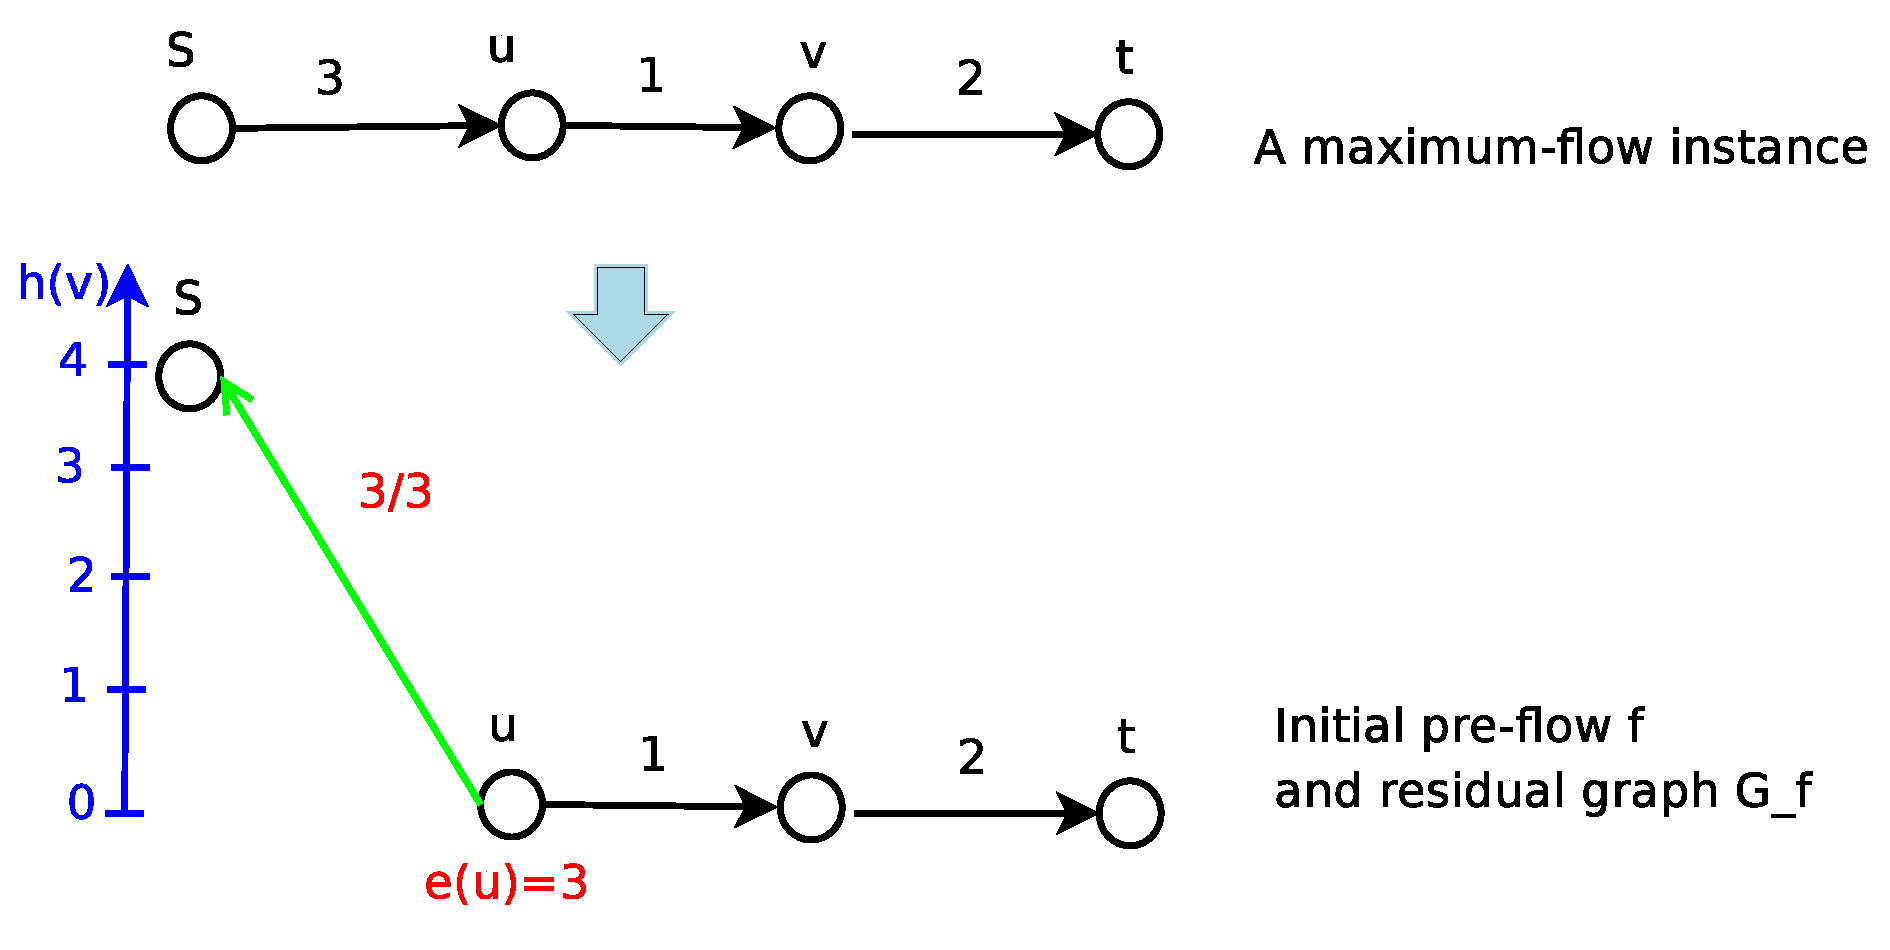
\includegraphics[width=3.5in] {L10-pushrelabelstep0.eps}
%\end{figure}
%
%} 
%
%
%\frame{
%\frametitle{A demo of push-relabel algo: Step 1}
%
%
%\begin{figure}
% 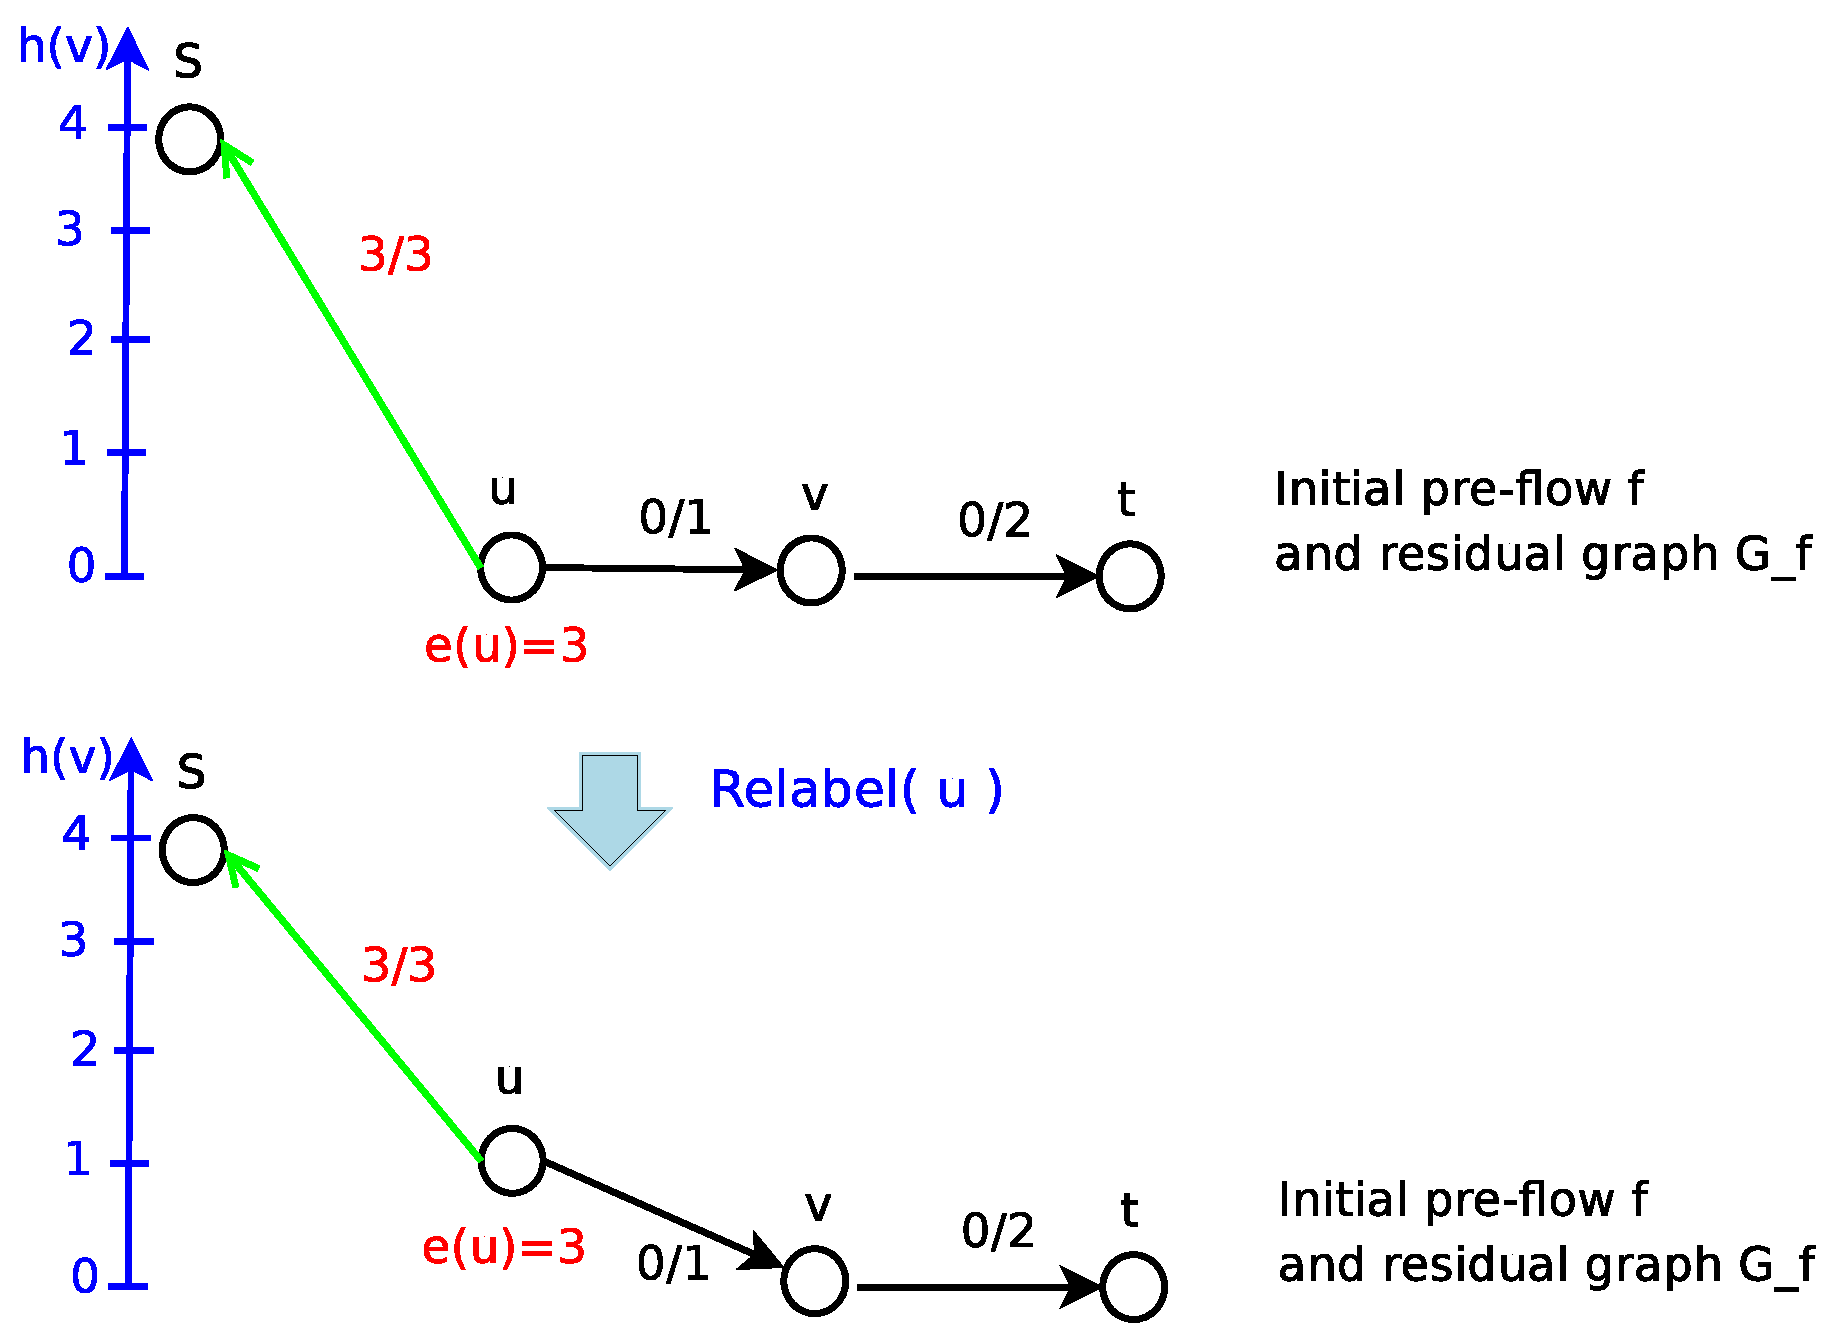
\includegraphics[width=3.2in] {L10-pushrelabelstep1.eps}
%\end{figure}
%} 
%
%
%\frame{
%\frametitle{A demo of push-relabel algo: Step 2}
%
%\begin{figure}
% 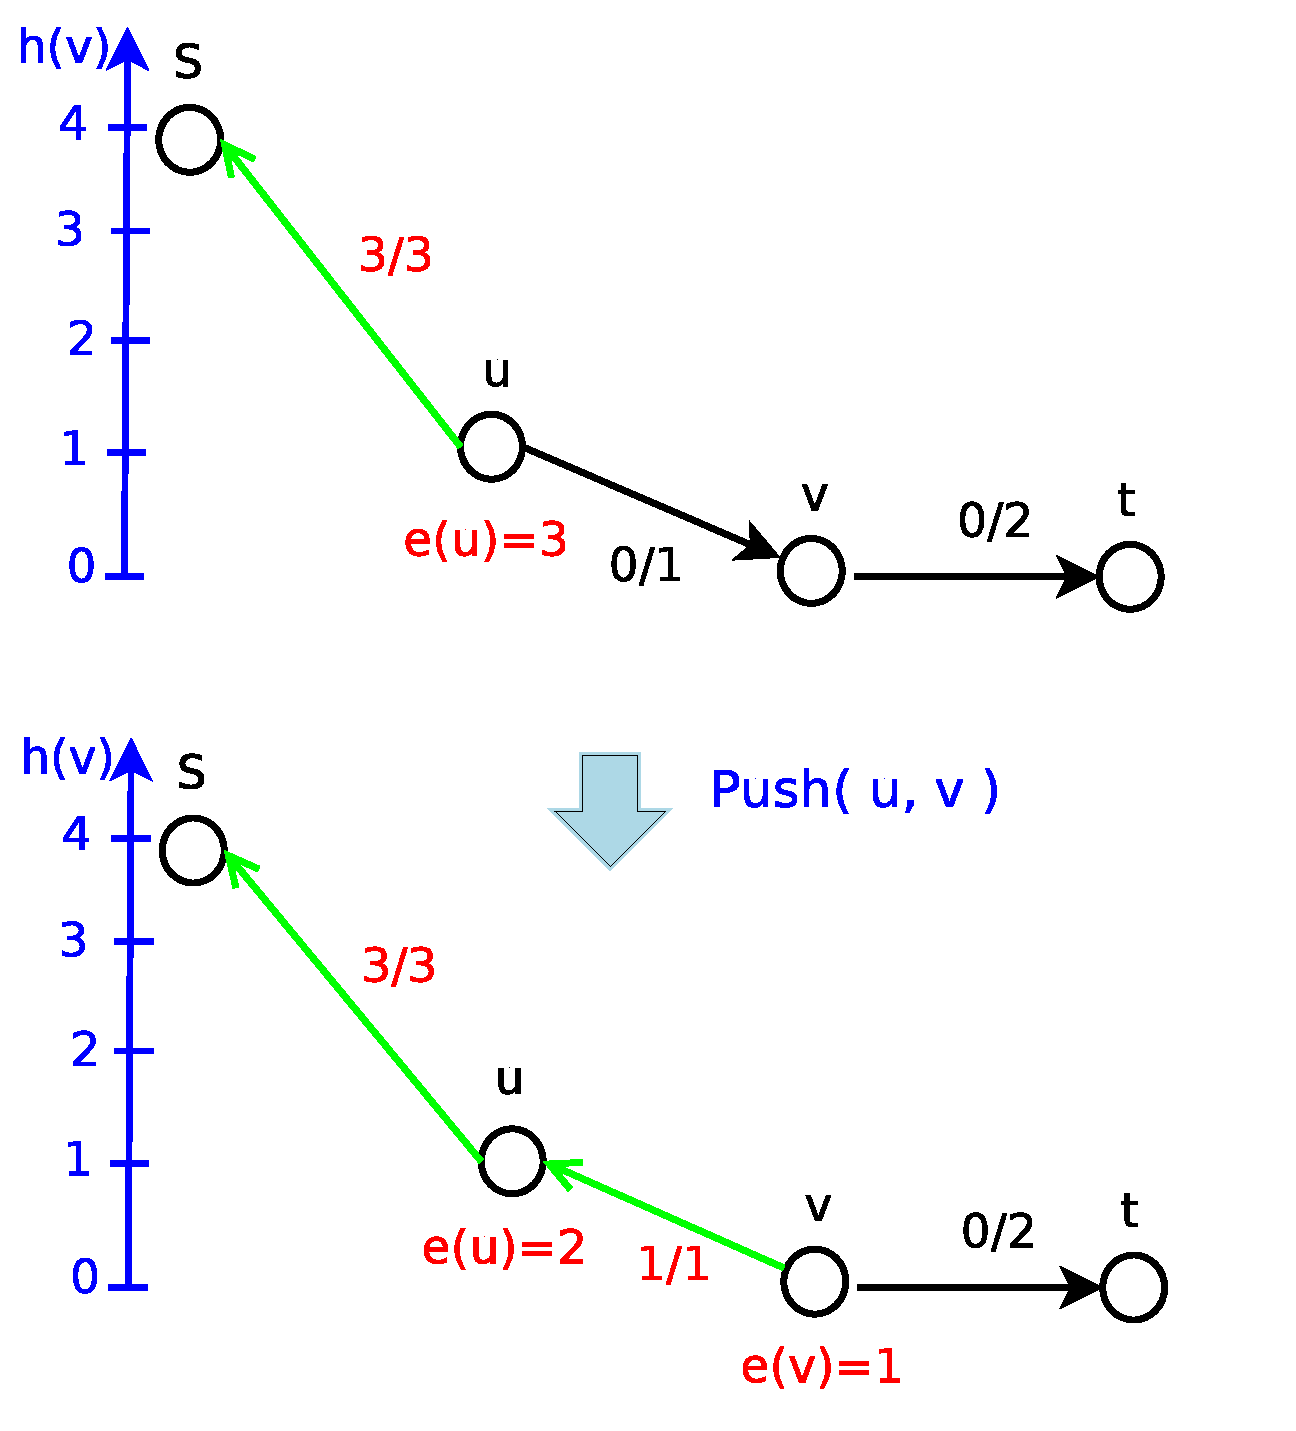
\includegraphics[width=2.8in] {L10-pushrelabelstep2.eps}
%\end{figure}
%} 
%
%
%\frame{
%\frametitle{A demo of push-relabel algo: Step 3}
%
%\begin{figure}
% 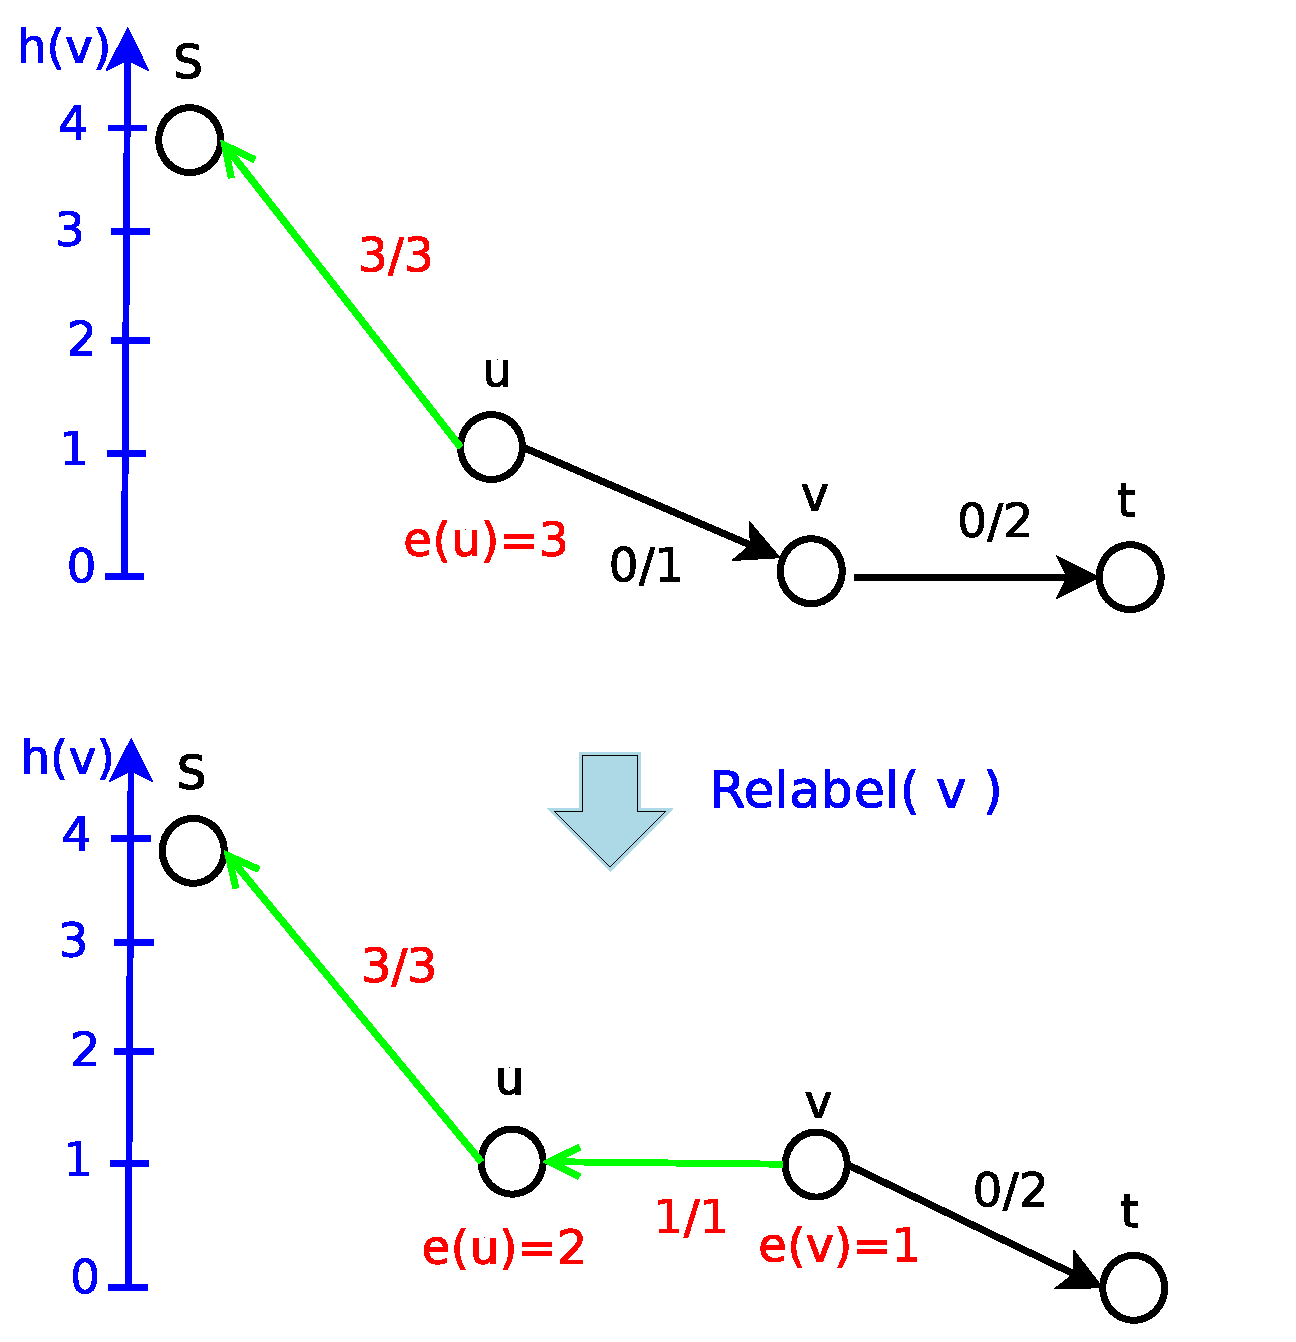
\includegraphics[width=2.8in] {L10-pushrelabelstep3.eps}
%\end{figure}
%} 
%
%
%\frame{
%\frametitle{A demo of push-relabel algo: Step 4}
%
%\begin{figure}
% 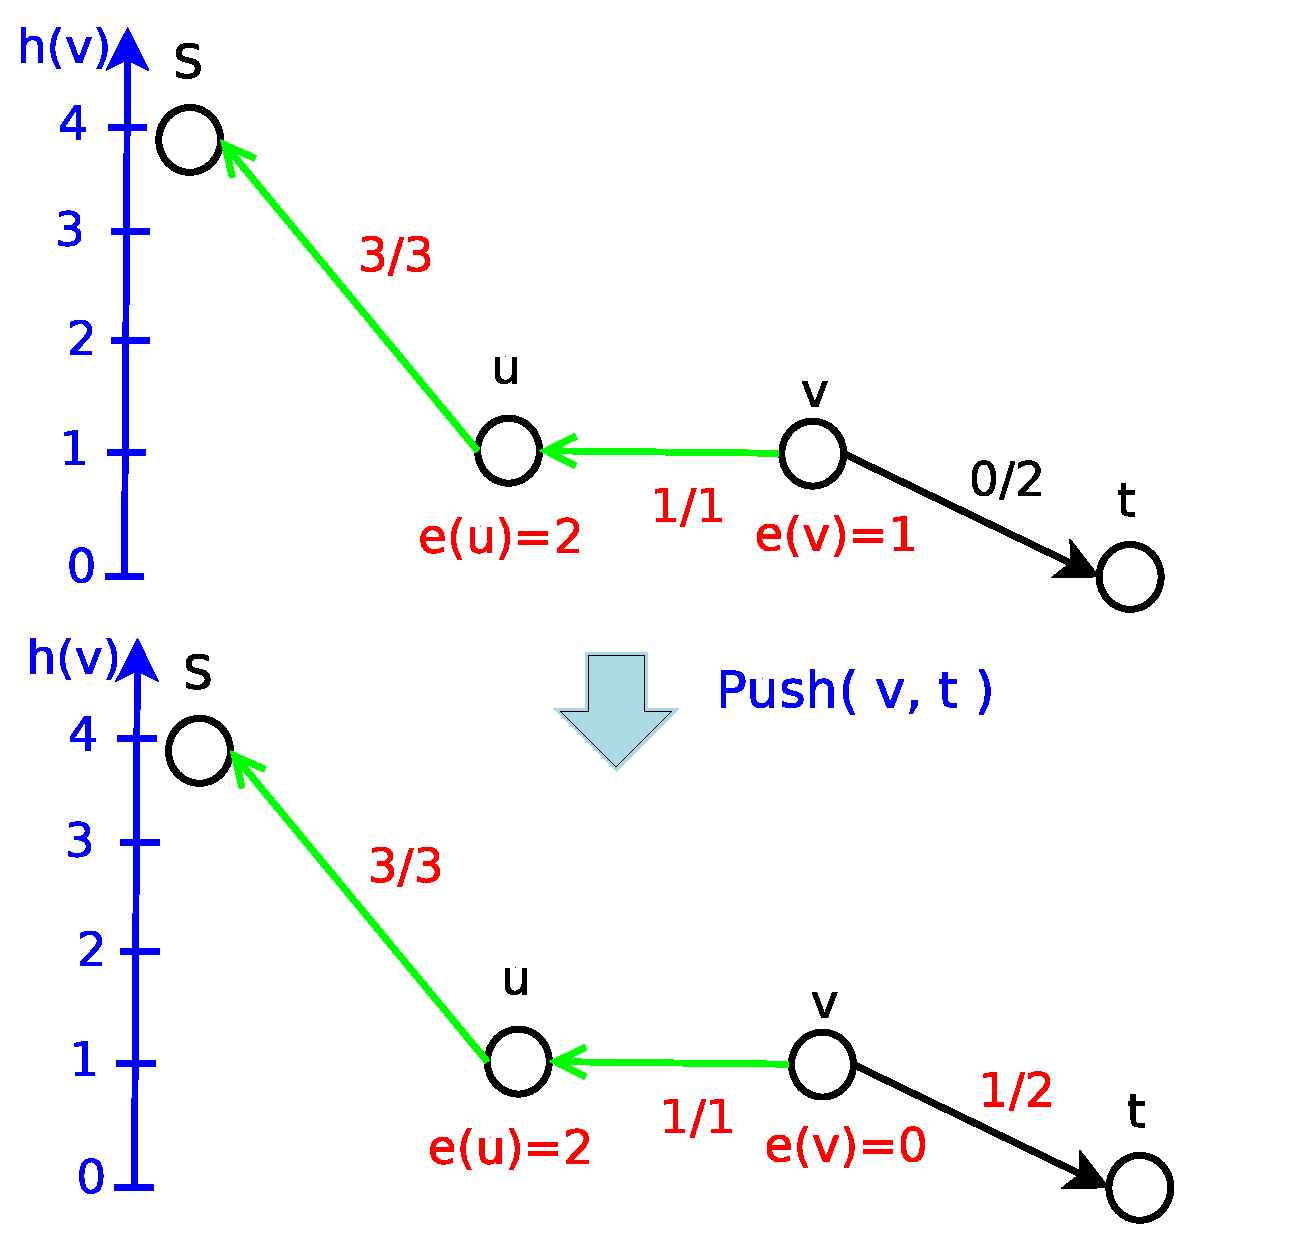
\includegraphics[width=2.8in] {L10-pushrelabelstep4.eps}
%\end{figure}
%} 
%
%
%\frame{
%\frametitle{A demo of push-relabel algo: Step 5}
%
%\begin{figure}
% 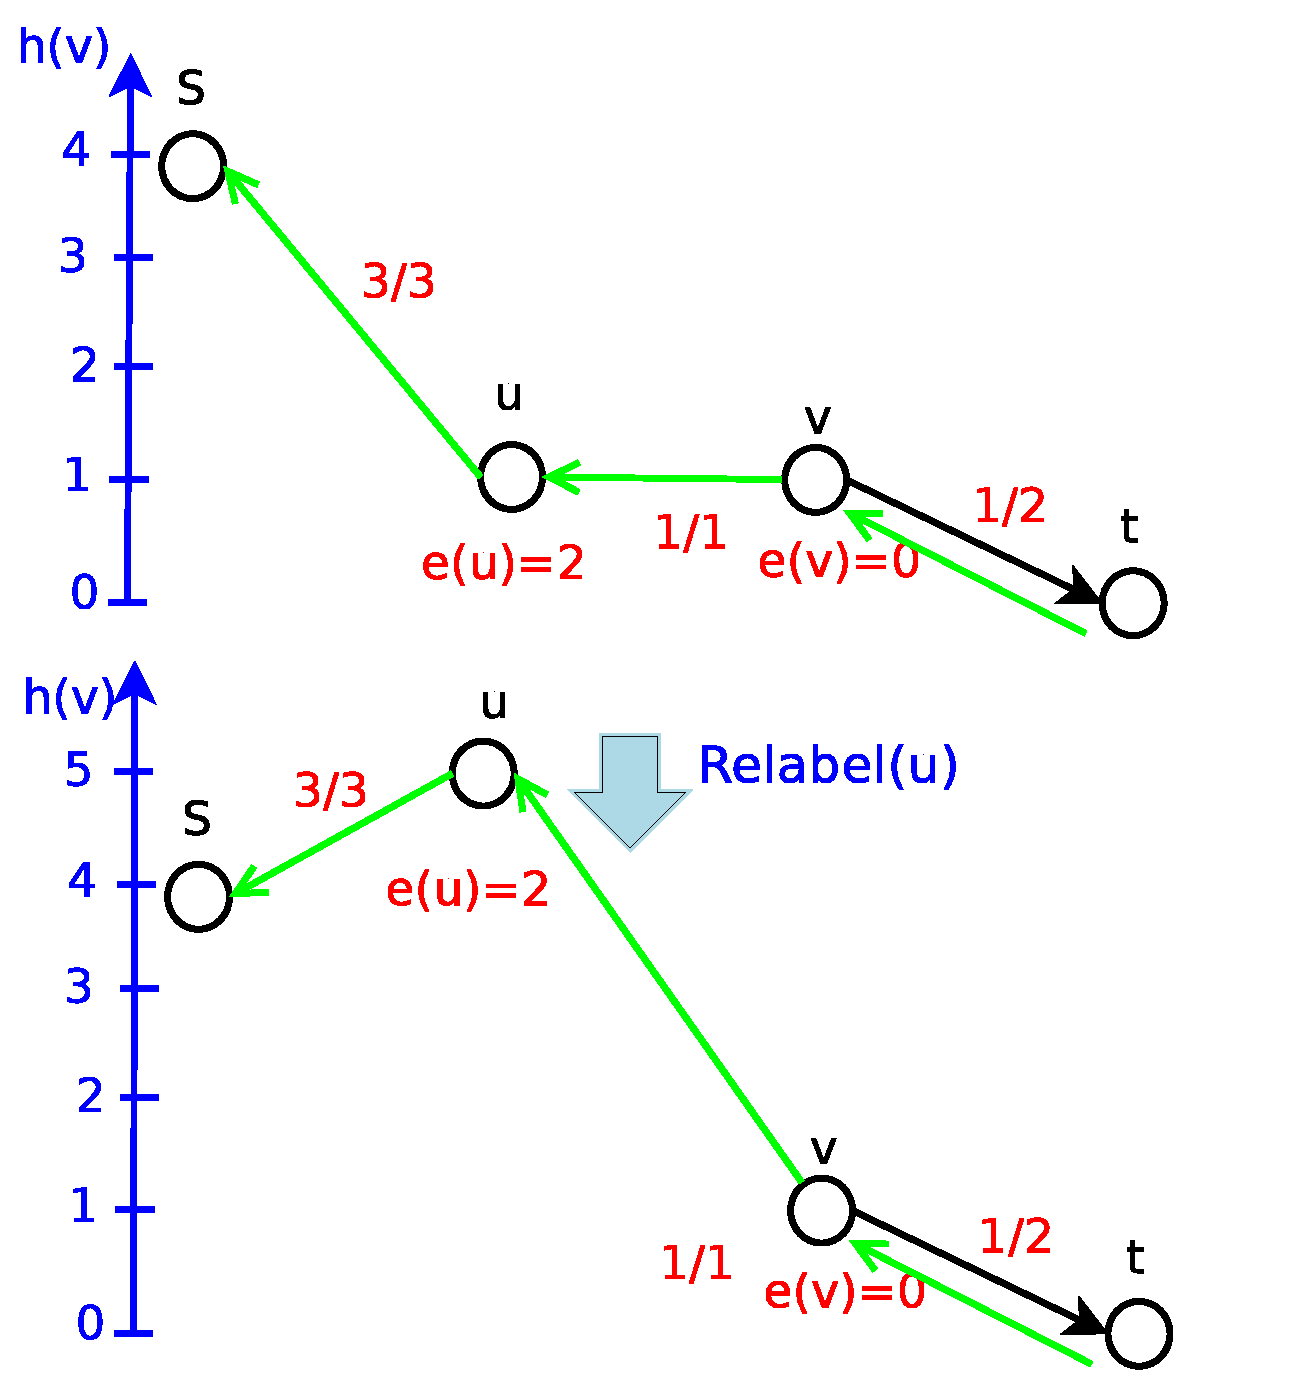
\includegraphics[width=2.7in] {L10-pushrelabelstep5.eps}
%\end{figure}
%
%}
%
%\frame{
%\frametitle{A demo of push-relabel algo: Step 6}
%
%\begin{figure}
% 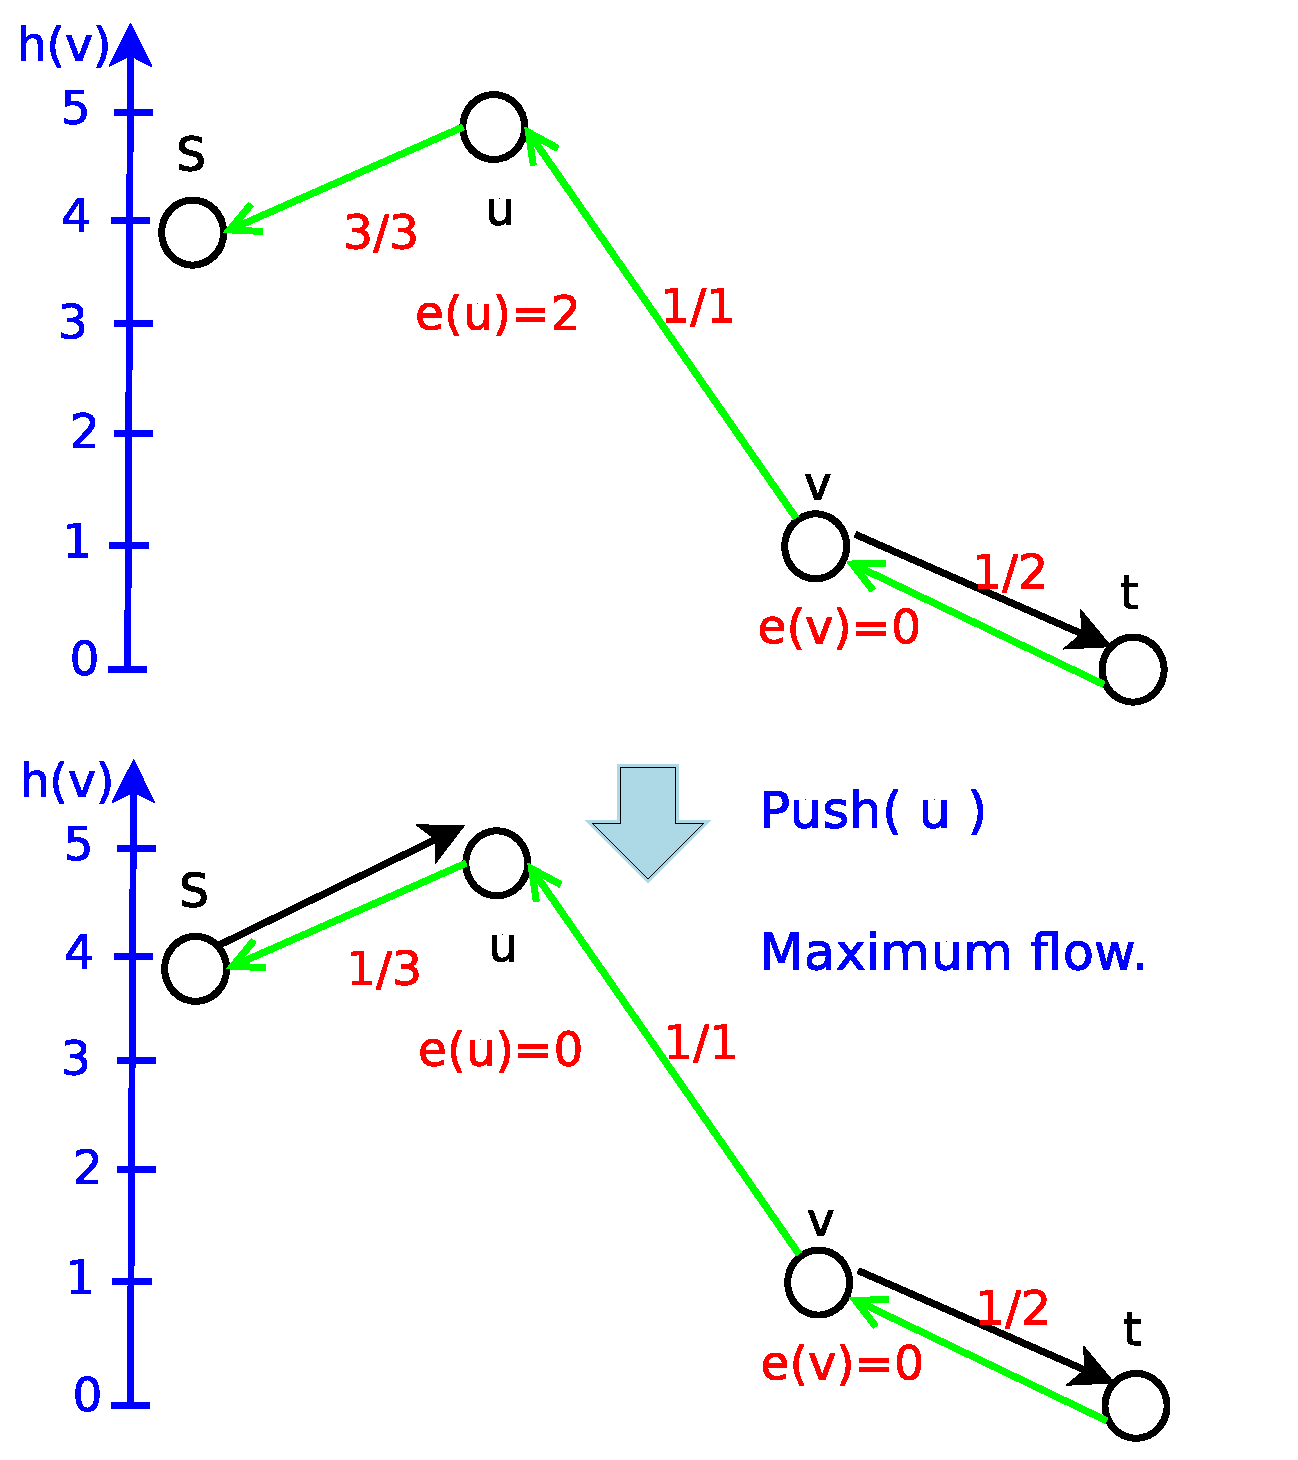
\includegraphics[width=2.7in] {L10-pushrelabelstep6.eps}
%\end{figure}
%
%}

\frame[allowframebreaks]{
\frametitle{Correctness }
\begin{Theorem}
 {\sc Push-relabel} algorithm keeps label valid, and thus outputs a maximum flow when ends. 
\end{Theorem}
\begin{Proof}
 (Induction on the number of push and relabel operations.)
 
 \begin{itemize}
  \item Push operation: the new $f$ is still a preflow since the capacity condition still holds. \\
  $Push(f,v,w)$ may add edge $(w,v)$ into $G_f$. We have $h(w) < h(v)$. (pre-condition). Thus, the label is valid for the new $G_f$.  
  \item Relabel operation: The pre-condition implies $h(v) \leq h(w) $ for any $(v,w)\in G_f$.  $relabel(f,h,v)$ changes $h(v)=h(v)+1$. Thus, the new $h(v) \leq h(w) + 1$.  
 \end{itemize}
\end{Proof}
}

\frame[allowframebreaks]{
\frametitle{Time-complexity: $\#Relabel$}
\begin{Theorem}
For any node $v$, $\#Relabel \leq 2n-1$. Thus, the total label operation number is less than $2n^2$. 
\end{Theorem}
\begin{Proof}
\begin{enumerate}
\item (Connectivity): For a node $w$ with $E_f(w) > 0$, there should be a path from $w$ to $s$ in $G_f$. \\
(Intuition: node $w$ obtain a positive $E_f(w)$ through a node $v$ by $Push(f, v, w)$. This operation also causes edge $(w,v)$ to be added into $G_f$. Thus, there should be a path from $w$ to $s$. ) 
\item (Upper bound of $h(v)$): $h(v) < 2n-1$ since there is a path from $v$ to $s$. The length of the path is less than $n-1$,  $h(s) =n$, and $h(v) \leq h(w)+1$ for any edge $(v,w)$ in $G_f$. 
\end{enumerate}
\end{Proof}
}


\frame[allowframebreaks]{
\frametitle{Time-complexity: $\#Push$}
Two types of $Push$ operations:
\begin{enumerate}
\item Saturated  push (s-push): if $Push(f,v,w)$ causes $(v,w)$ removed from $G_f$. 
\item Unsaturated push (uns-push): other pushes. 
\end{enumerate}
$\#Push=\#s$-$push + \#uns$-$push$. 

\begin{Theorem}
 $\#s$-$push \leq 2nm$. 
\end{Theorem}
\begin{Proof}
 Consider an edge $e=(v,w)$. We will show that during the execution of algo, $(v,w)$ appears in $G_f$ at most $2n$ times. 
 \begin{itemize}
  \item (Removing): a saturated  $Push(f, v, w)$ removes $(v,w)$ from $G_f$. We have $h(v)=h(w)+1$. 
  \item (Adding): Before applying $Push( f, v, w)$ again, $(v,w)$ should be added to $G_f$ first. The only way to add $(v,w)$ to $G_f$ is $Push( f, w, v)$. The pre-condition of $Push(f, w, v)$ requires that $h(w)  \geq h(v) + 1$, i.e., $h(w)$ should be increased at least $2$ since the previous $Push( f, v, w)$ operation. And we have $h(w) \leq 2n-1$. 
 \end{itemize}
\end{Proof}


}

\frame[allowframebreaks]{
\frametitle{Time-complexity: $\#Push$}
\begin{Theorem}
 $\#uns$-$push \leq 2n^2m$. 
\end{Theorem}
\begin{Proof}
Define a measure $\Phi(f,h) = \sum_{v: E_f(v) > 0} h(v)$. 
\begin{itemize}
 \item (Increase and upper bound) $\Phi(f,h) < 4n^2m$: 
 \begin{enumerate} 
  \item Relabel: a relabel operation increase $\Phi(f,h)$ by 1. The total $O(2n^2)$ relabel operations increase $\Phi(f,h)$ at most $O(2n^2)$. 
  \item Saturized push: A saturated $Push(f, v, w)$ operation increases $\Phi(f,h)$ by $h(w)$ since $w$ has excess now. $h(w) \leq 2n-1$ implies an upper bound for each operation. The total $2nm$ saturated pushes increase $\Phi(f,h)$ by at most $4n^2m$.
 \end{enumerate}

 \item (Decrease) An unsaturated $Push(f, v, w)$ will reduce $\Phi(f,h)$ at least $1$. \\
 (Intuition: after unsaturated $Push(f, v, w)$, we have $E_f(v) = 0$, which reduce $h(v)$ from $\Phi(f,h)$; on the other side, $w$ obtains excess from $v$, which will increase $\Phi(f,h)$ by $h(w)$. From $h(v) \leq h(w) + 1$, we have that $\Phi(f,h)$ reduces at least $1$.)
\end{itemize}

\end{Proof}

Time complexity: $O(n^2m)$. 
}

%\frame{
%\begin{block}{}
% Extensions of {\sc MaxFlow} problem
%\end{block}
%
%}
%
%\frame{
%\frametitle{Three extension of {\sc MaxFlow} problem}
%
%\ \\
%\ \\
%\ \\
%\begin{block}{}
% \begin{enumerate}
%  \item {\sc MaxFlow} for indirected graph; \\
%  \ \\
%  \item Multiple sources and multiple sinks; \\
%  \ \\
%  \item Lower bound of capacity; 
% \end{enumerate}
%\end{block}
%}
%
%\frame{
%\frametitle{Extension 1:  Indirected graph}
%
%\begin{itemize}
% \item 
%Reduction: changing an indirected graph $G$ to a directed graph $G'$ through: 
%\begin{enumerate}
% \item edges:  for each edge $(u,v)$ of $G$, introducing two edges $e=(u,v)$ and $e'=(v,u)$ to $G'$; 
%\item capcities: setting $C(e')=C(e)$. 
%\end{enumerate}
%\item Algorithm: we first calculate maximum flow $f'$ for network $G'$; then transform $f'$ to $f$ through the following operation. We will show that $f$ is the maximum flow of network $G$.  
%
%\begin{figure}
% 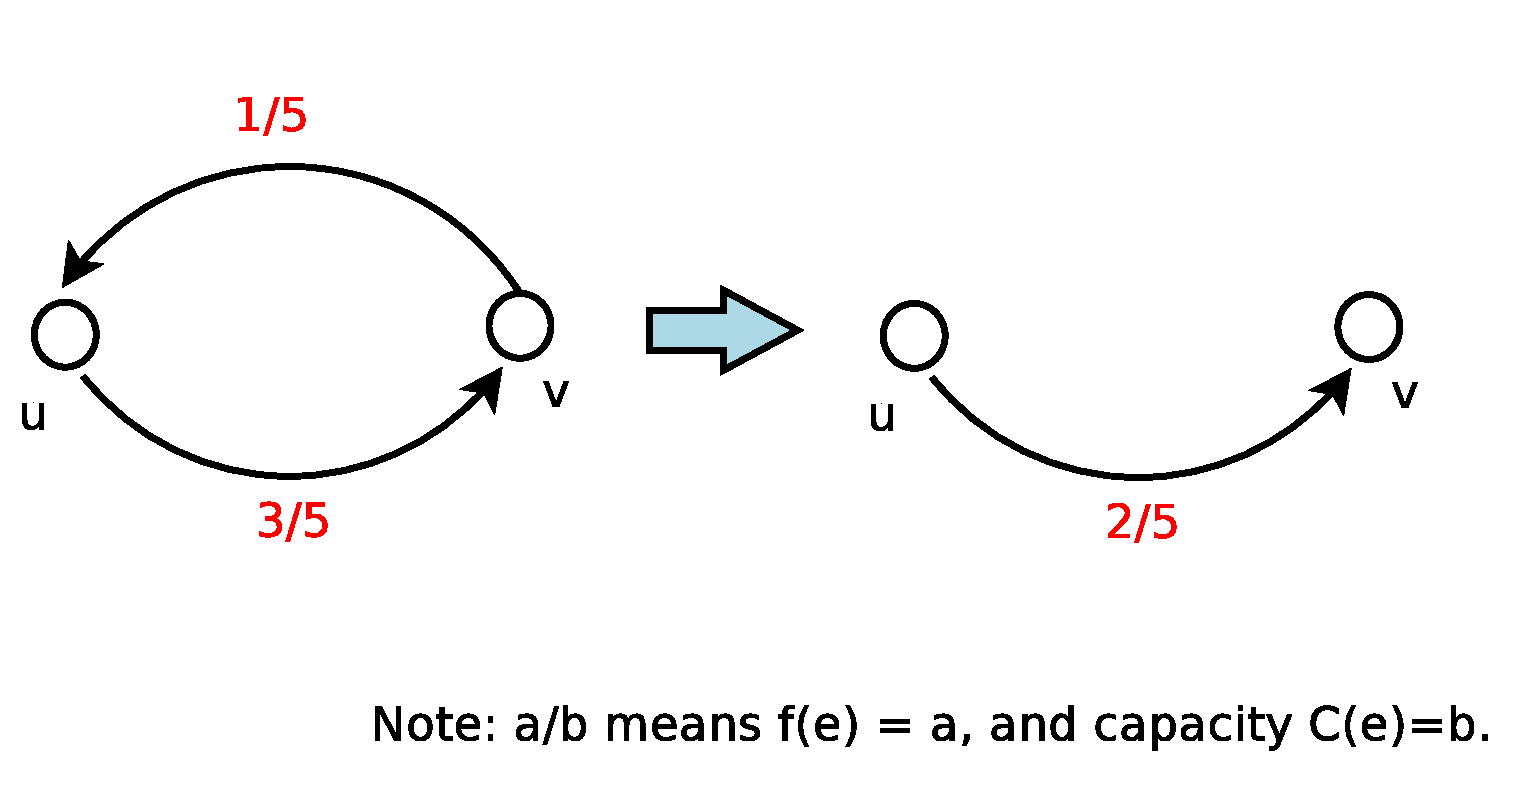
\includegraphics[width=3in] {L10-indirectedgraph.eps}
%\end{figure}
%\end{itemize} 
%} 
% 
%\frame{
%\frametitle{Extension 1:  Indirected graph cont'd}
%
%Key observation: there exists a maximum flow that uses at most one of the two opposite edges. Formally, we have: 
%
%\begin{Theorem}
% There exists a maximum flow $f$ for network $G$, where $f(u,v) = 0$ or $f(v,u)=0$. 
%\end{Theorem}
%\begin{Proof}
%\begin{itemize}
%\item Suppose $f'$ is a maximum flow for network $G'$, where $f'(u,v) > 0$ and $f'(v,u) > 0$. We change $f'$ to $f$ as follows: 
%\item Let $\delta=\min\{f'(u,v), f'(v,u) \}$. 
%\item Define $f(u,v) = f'(u,v) - \delta$, and $f(v,u) = f'(v,u) - \delta$. 
%\item $f$ has the same value to $f'$ and thus optimal. In the meanwhile, $f(u,v) = 0$ or $f(v,u)=0$. 
%\end{itemize}
%\end{Proof}
%}
%
%\frame[allowframebreaks]{
%\frametitle{Extension 2: {\sc Circulation} problem with multiple sources and multiple sinks}
%
%
%\begin{block}{}
%{\bf INPUT: } a network $G=<V, E>$, each edge $e$ has a capacity $C(e) > 0$, multi sources $s_i$ and sinks $t_j$. A sink $t_j$ has demand $d_j > 0$, while a source $s_i$ has supply ( described as $d_i < 0$). For the sake of simplicity, we define $d_v=0$ for other nodes. Thus we have $\sum_i d_i = 0$, and define $D=\sum_{d_v >0 } d_v$ be the {\it total demands }. \\ 
%{\bf OUTPUT: } a circulation $f$ to satisfy all demands using the availale supply, i.e., 
%\begin{enumerate}
% \item (Capacity condition):  $0 \leq f(e) \leq C(e)$;
% \item (Demand condition):  $f^{in} (v) - f^{out} (v) = d_v$; 
%\end{enumerate}
%\end{block}
%
%\textcolor{red}{Note: {\sc Circulation} differs from {\sc MultiCommodities} problem in that there is ONLY one commodity. In other words, a sink can accept commodity from any source. Contrastly, in {\sc MultiCommodities} problem, $t_i$ only accepts commodity $k_i$ from $s_i$. }
% 
%Reduction: constructing a network $G'$ through adding a super source $s^*$ to connect each $s_i$ with capacity $C(s^*,s_i)=-d_i$. Similarly, adding a super sink $t^*$ to connect to each $t_j$ with capacity $C(t_j,t^*)=d(t_j)$. 
%
%\begin{figure}
% 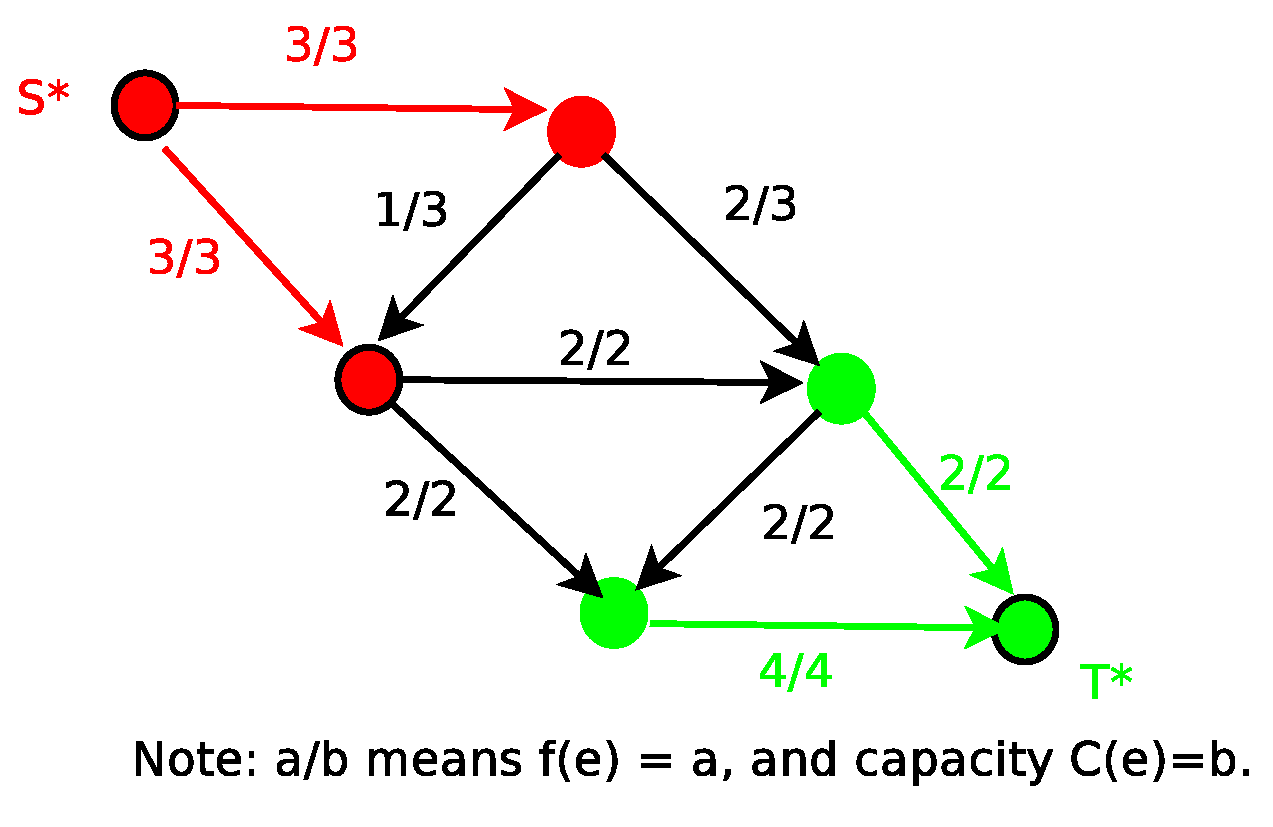
\includegraphics[width=3in] {L10-circulationtomaximumflow.eps}
%\end{figure}
%
%\begin{Theorem}
%There is a feasible solution to {\sc Circulation} problem iff the maximum $s^*-t^*$ flow in $G'$ is $D$. 
%\end{Theorem}
%\begin{Proof}
%\begin{itemize}
% \item 
%$\Leftarrow$: \\ 
%  Simply removing all $(s^*,s_i)$ and $(t_j,t^*)$ edges. \\
%
%\item 
%$\Rightarrow$: \\ 
%\begin{enumerate}
% \item 
%Define a flow $f$ as follows: $f(s^*,s_i)=-d_i$ and $f(t_j, t^*)=d_j$. \\
%\item 
%Consider cut $(S, \bar{S})$, where $A=\{s^*\}$. 
%\item 
%We have $C(S, \bar{S})=D$. Thus $f$ is a maximum-flow since it reaches the maximum value.
%\end{enumerate}
%\end{itemize}
% 
%\end{Proof}
%}
%
%\frame{
%\frametitle{Extension 3: Lower bound of capacity}
%
%
%\begin{block}{}
%{\bf INPUT: } a network $G=<V, E>$, each edge $e$ has a capacity upper bound $C(e) > 0$, and capacity lower bound $L(e)>0$, multiple sources $s_i$ and sinks $t_j$. A sink $t_j$ has demand $d_j > 0$, while a source $s_i$ has supply ( described as $d_i < 0$). For the sake of simplicity, we define $d_v=0$ for other nodes. Thus we have $\sum_i d_i = 0$, and define $D=\sum_{d_v >0 } d_v$ be the {\it total demands }. \\ 
%{\bf OUTPUT: } a circulation $f$ to satisfy all demands using the availale supply, i.e., 
%\begin{enumerate}
% \item (Capacity condition):  $L(e) \leq f(e) \leq C(e)$;
% \item (Demand condition):  $f^{in} (v) - f^{out} (v) = d_v$; 
%\end{enumerate}
%\end{block}
%
%Intuition: for each edge $e$, we require $L(e) \leq f(e) \leq C(e)$. By setting lower bound, we can force edge $e$ to be used by flow. 
%}
%
%
%\frame{
%\frametitle{Extension 3: Lower bound of capacity cont'd}
%
%Reduction: 
%\begin{enumerate}
%\item 
%We build an initial circulation $f_0$ by setting $f_0(e) = L(e)$. 
%\item 
%Next we improve $f_0$ to a circulation $f'$ through solve another {\sc Circulation} problem: construct a network $G'$ without lower bound restrictions on capacity, and demands $d'_v = d_v - L(w,v)$. \\
%\end{enumerate}
%\begin{figure}
% 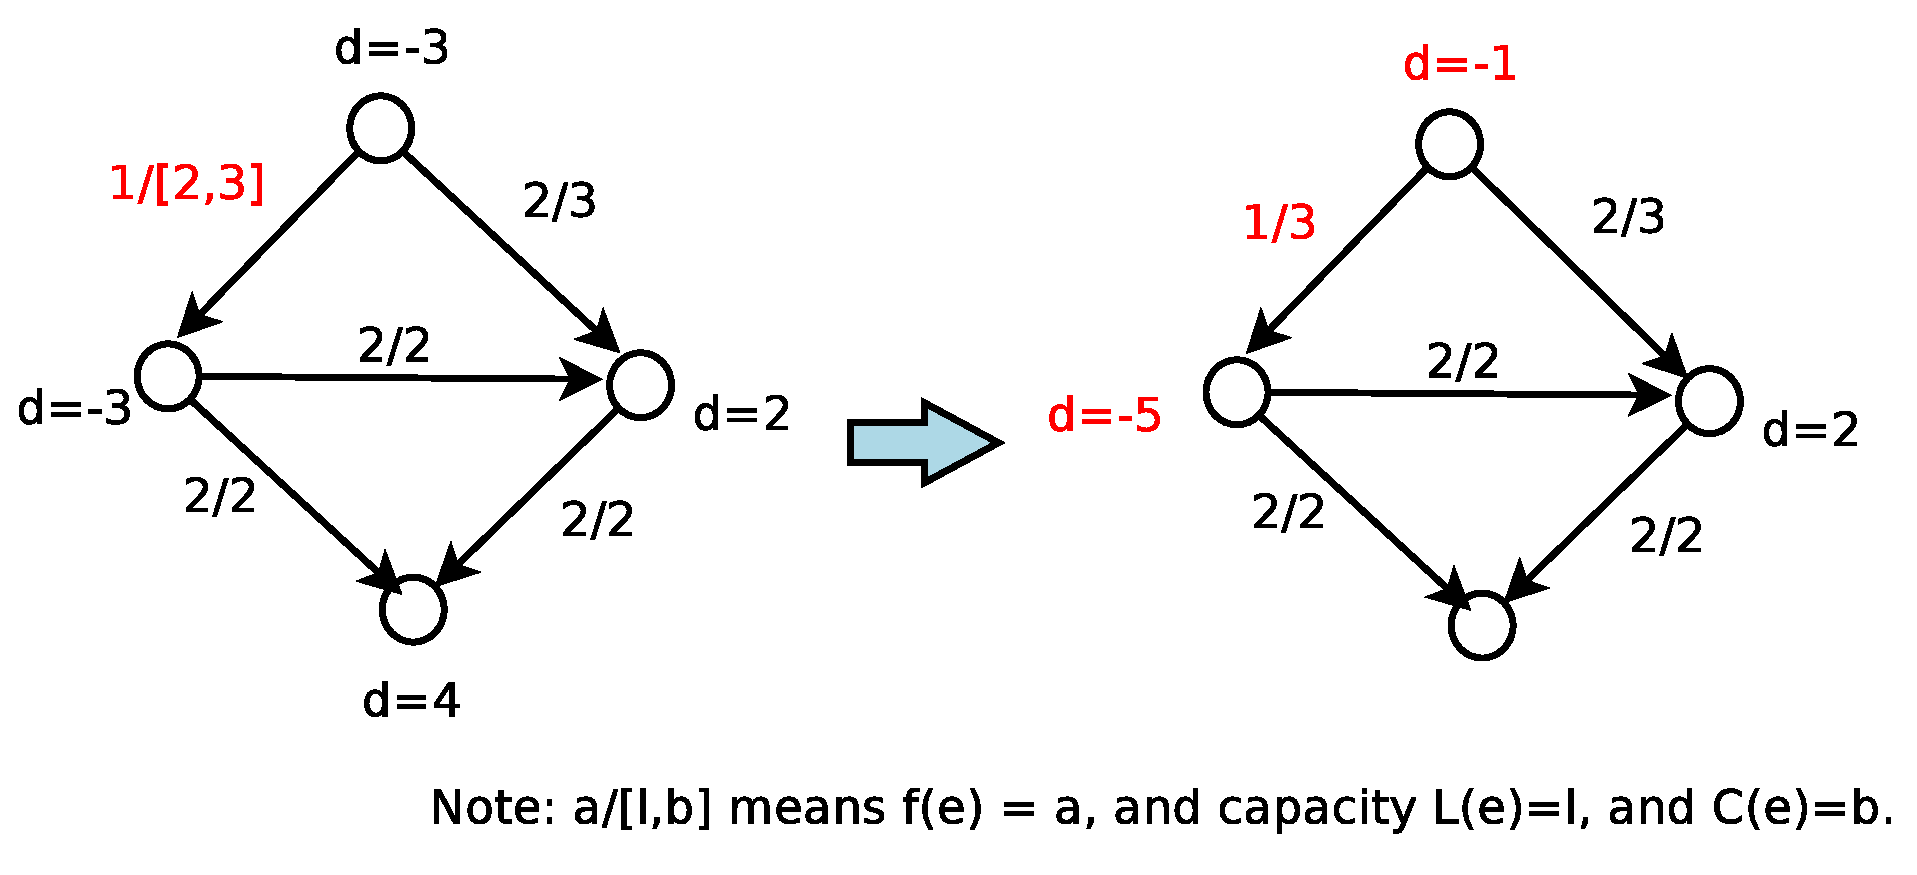
\includegraphics[width=2.8in] {L10-lowerboundcirculation.eps}
%\end{figure}
%} 
%
%
%\frame{
%\frametitle{Extension 3: Lower bound of capacity cont'd}
%
%
%\begin{Theorem}
% There is a circulation $f$ to $G$ (with lower bounds) iff there is a circulation $f'$ to $G'$. 
%\end{Theorem}
%\begin{Proof}
%Define $f'(e) = f(e)+L_e$. It is easy to verify both capacity and demand conditions. 
%\end{Proof}
%}
%
%\frame{
%\begin{block}{}
%{Applications of {\sc MaxFlow} problem } 
%\end{block}
%} 
%
%\frame{
%\frametitle{Applications of {\sc MaxFlow} problem }
%\ \\
%\begin{block}{}
%Formulating a problem into {\sc MaxFlow} problem: 
%\begin{enumerate}
% \item How to define $s$ and $t$? Sometimes a super source $s^*$ and $t^*$ are needed. 
% \item How to define capacity $L_e$ and $C_e$? 
% \item Sometimes minimum cut is more suitable than maximum flow.
% \item Need to prove that a maximum flow correspond to a solution to the original problem. 
%\end{enumerate}
%Note: most problems utilize the property that there exists a maximum integer-valued flow iff there exists a maximum flow. 
%\end{block}
%
%(See extra slides.)
%}

%
%\frame{
%\begin{block}{}
%	Extension: an instance with multiple optimal solution  
%\end{block} 
%} 
%
%\frame{
%\frametitle{Multiple optimal solutions  }
%
%\begin{itemize}
%\item For some instances, there might be multiple optimal solutions, i.e. multiple flow with the same maximum flow value. 
%\item In addition, these maximum flows might share some edges. In other words, these edges are ``necessary'' edges. 
%\item Sometimes, we need to enumerate all these optimal solutions, or get a small sample of these optimal solutions.  
%\end{itemize}  
%(See ppt for a demo)
%} 



\end{document}
